\chapter{Objets physiques de haut niveau}\label{chapter-HLO}

\section{Introduction}\label{chapter-HTT_analysis-section-introduction}
Dans le chapitre~\refChMSSM,
il a été montré que le modèle standard (SM, \emph{Standard Model}) souffre de lacunes quant à l'explication à apporter à certaines observations.
Certaines peuvent être comblées par des modèles allant au-delà (BSM, \emph{Beyond Standard Model}) comme l'extension supersymétrique minimale du modèle standard ou \og MSSM \fg.
Une des conséquences du MSSM est l'existence de cinq bosons de Higgs, dont trois neutres, \higgs, \Higgs\ et \HiggsA.
L'un d'entre-eux doit correspondre au boson découvert en 2012 et interprété comme étant le boson de Higgs du \SM~\cite{ATLAS_Higgs_discovery,CMS_Higgs_discovery,CMS_Higgs_discovery_2013,ATLAS-CMS-Higgs_combined_1,ATLAS-CMS-Higgs_combined_2}.
L'existence des deux bosons de Higgs neutres supplémentaires peut être testée expérimentalement avec des accélérateurs de particules,
comme cela a été fait au LEP~\cite{Schael:2006cr}.
Ces bosons se désintègrent préférentiellement en paire de quarks~\quarkb\ ou de leptons~\tau.
Bien que le rapport de branchement (\BR) de ces bosons aux \quarkb\ soit 5 à 10 fois supérieur que celui aux \tau,
ces derniers proposent une meilleure accessibilité expérimentale dans les collisionneurs hadroniques comme le Tevatron,
ou ces désintégrations en \tau\ ont été étudiées~\cite{Aaltonen:2009vf,Abazov:2011jh}.
\par
L'expérience CMS installée au LHC et présentée dans le chapitre~\refChLHCCMS\ permet elle aussi de tester expérimentalement le MSSM, dans des conditions de collision inédites.
La recherche de bosons de Higgs supplémentaires se désintégrant en paire de \tau\ a été menée dans les collisions de protons avec une énergie dans le centre de masse de $\sqrt{s}=\num{7}$ et $\SI{8}{\TeV}$ (Run~I) \cite{Chatrchyan:2012vp,CMS-MSSM-HTT_2014,CMS-PAS-HIG-13-021,CMS-PAS-HIG-14-029} ainsi qu'avec les données récoltées en 2016 avec une énergie de $\sqrt{s}=\SI{13}{\TeV}$ \cite{CMS-PAS-HIG-17-020}.
Plusieurs thèses portent sur l'analyse des événements où un boson de Higgs se désintègre en paire de \tau~\cite{Gael_thesis,Artur_thesis}.
La désintégration en paire de \quarkb\ est également exploitée~\cite{Chatrchyan:2013qga,Khachatryan:2015tra},
ainsi que celle en paire de muons~\cite{CMS:2015ooa}.
L'expérience ATLAS mène des recherches similaires~\cite{Aad:2012cfr,ATLAS-MSSM-HTT_2018,ATLAS-MSSM-HTT_2020}.
\par
Ce chapitre présente la
recherche de bosons de Higgs supplémentaires de haute masse se désintégrant en paire de \tau\
avec les données récoltées par l'expérience CMS
lors du Run~II du LHC (années 2016, 2017 et 2018),
correspondant à une luminosité intégrée de \SI{137}{\femto\barn^{-1}} ($\num{35.9}+\num{41.5}+\SI{59.7}{\femto\barn^{-1}}$)
à une énergie dans le centre de masse de $\sqrt{s}=\SI{13}{\TeV}$.
Sur les six canaux de désintégration de la paire de leptons \tau\ introduits dans le chapitre~\refChMSSM,
les quatre présentant les plus grands \BR\ sont considérés dans l'analyse.
Il s'agit des canaux
hadronique (\tauh\tauh),
semi-leptoniques (\mu\tauh, \ele\tauh)
et
leptonique asymétrique (\ele\mu).
Les canaux leptoniques symétriques (\mu\mu, \ele\ele) ne sont pas exploités.
\par
Dans les données réelles, les particules doivent forcément être reconstruites à partir des signaux qu'elles produisent dans le détecteur.
Dans le cas des données simulées, la réponse du détecteur aux particules est modélisée.
À partir des signaux réels comme simulés, les particules individuelles sont reconstruits comme exposé dans le chapitre~\refChLHCCMS.
Elles permettent d'obtenir les objets physique de haut niveau, introduits chapitre~\refChJERC, que sont l'énergie transverse manquante (MET), les jets et les taus hadroniques (\tauh).
Les simulations n'étant pas exemptées de défauts, des corrections déterminées à l'aide d'analyses annexes leurs sont appliquées.
Les corrections spécifiques à la présente analyse sont présentées dans la section~\ref{chapter-HTT_analysis-section-corrections}.
Les autres corrections sont introduites dans le chapitre~\refChLHCCMS.
Les objets reconstruits et corrigés permettent de sélectionner les événements d'intérêt pour l'analyse selon la procédure explicitée en section~\ref{chapter-HTT_analysis-section-selection}.
Des processus physiques différents de ceux du signal recherché passent cette sélection et constituent le bruit de fond.
Afin d'interpréter les observations, il est nécessaire de modéliser ce bruit de fond.
Cette modélisation est présentée section~\ref{chapter-HTT_analysis-section-bg_estimation}.
En plus de l'utilisation de données simulées, des techniques basées sur les données réelles sont exploitées.
Des données dites \og encapsulées \fg{} (\emph{embedded}) sont ainsi produites selon la procédure exposée section~\ref{chapter-HTT_analysis-section-bg_estimation-embedding} et décrivent les événements contenant une vraie paire de leptons \tau.
Une estimation du bruit de fond dû aux jets identifiés à tort comme des taus hadroniques (\ftauhs) est quant à elle obtenue grâce à la méthode des facteurs de faux (\emph{fake factors}) introduite section~\ref{chapter-HTT_analysis-section-bg_estimation-FF_method}.
Les événements sont par la suite catégorisés afin d'augmenter la sensibilité de l'analyse.
Les catégories utilisées sont présentées en section~\ref{chapter-HTT_analysis-section-categorisation}.
Les sources d'incertitudes systématiques sont données section~\ref{chapter-HTT_analysis-section-systematics}.
Leur prise en compte dans l'extraction du signal ainsi que la modélisation de celui-ci sont exposée dans la section~\ref{chapter-HTT_analysis-section-signal_extraction}.
Enfin, les résultats obtenus sont disponibles section~\ref{chapter-HTT_analysis-section-results}.
Certains sont indépendants de tout modèle, d'autres sont obtenus dans le cadre de scénarios spécifiques au MSSM~\cite{Bagnaschi_2019}.
\par
Une note d'analyse (CMS AN 2020/218) \cite{CMS-NOTE-2020-218} est déjà disponible pour les membres de la collaboration et un article est en préparation~\cite{HIG-21-001}.
Ces travaux sont réalisés au sein d'une équipe regroupant:
\begin{itemize}
\item l'Institut de Physique des 2 Infinis (IP2I) de l'Université Claude Bernard de Lyon, mon laboratoire de rattachement;
\item l'\emph{Institut für Experimentelle Teilchenphysik} (ETP) du \emph{Karlsruher Institut für Technologie} (KIT) de Karlsruhe;
\item le \emph{Deutsches Elektronen-Synchrotron} (DESY) de Hambourg;
\item l'\emph{Imperial College} de Londres;
\item l'\emph{Institut für Hochenergiephysik} (HEPHY)
% de l'\emph{Österreichische Akademie der Wissenschaften}
 de Vienne;
\item le \emph{Tata Institute of Fundamental Research} de Bombay.
\end{itemize}
\par
En début de thèse, j'ai travaillé sur les données de l'année 2017 en équipe avec Gaël \textsc{Touquet} qui a exploité le canal \tauh\tauh\ dans sa thèse~\cite{Gael_thesis}.
Je me suis concentré sur les  canaux semi-leptoniques et plus particulièrement le canal \mu\tauh.
La présence de \tauh\ dans nos canaux respectifs nous a mené à de travailler en étroite collaboration.
Les événements étaient analysés à l'aide d'un code basé sur \HEPPY~\cite{heppy},
indépendant de celui utilisé par les autres instituts listés précédemment,
ce qui a permis à l'ensemble des acteurs de cette analyse de valider la bonne implémentation des différentes corrections et sélections détaillées dans ce chapitre.
À cette occasion, j'ai découvert une erreur dans le code de \COMBINE.
Cette erreur a été comprise et corrigée.
Le correctif~\cite{BBB_PR} a été transmis à la collaboration CMS qui l'a pris en compte.
\par
J'ai par la suite travaillé directement avec le groupe de Karlsruhe dans le cadre de l'analyse du Run~II.
J'ai implémenté le traitement du scénario avec violation de la symétrie $CP$.
J'ai de plus participé au traitement des jeux de données utilisés, listés dans l'annexe~\refApHTTdatasets.
Il s'agissait de s'assurer du bon déroulement de plusieurs milliers de tâches informatiques et du regroupement de leurs résultats.
Enfin, j'ai activement participé à la rédaction de la note d'analyse CMS correspondante~\cite{CMS-NOTE-2020-218}.
%Homework concerning the bbH and ggH samples
%1) Monitor the production ---> ask in case there are invalid samples
%2) Process the new samples
%3) Rederive the ggH weights based on input POWHEG samples
%4) Update the signal modelling for new samples in CombineHarvester
%And on the experimental side I recall:
%newes FF's
%MET tail correction and uncertainty
%Are these the only items left before wrapping up or am I missing anything in addition?

\subsection{Énergie transverse manquante}\label{chapter-LHC-section-evt_reco-subsec-MET}


\section{Formation des jets}\label{chapter-JERC-section-jets}
Lorsqu'un parton est issu de la collision, cette particule possède une haute énergie.
Il radie alors, par interaction forte, d'autres partons.
Par conservation, l'énergie portée par chaque parton ainsi obtenu diminue et par conséquent, $g_s$ augmente.
\par Tant que l'échelle d'énergie est suffisamment grande pour que $g_s \ll 1$, ce qui correspond à des énergies supérieures à la centaine de \SI{}{\MeV}, il est possible de réaliser des calculs perturbatifs.
La radiation de partons créé la \og gerbe partonique \fg, sujet de la prochaine section.
\par Au fur et à mesure des radiations, l'échelle en énergie diminue et en deçà d'une centaine de \SI{}{\MeV}, il n'est plus possible de réaliser des calculs perturbatifs car $g_s$ augmente.
Des modèles paramétriques sont alors utilisés pour caractériser le phénomène d'\og hadronisation \fg, abordés ensuite.

\subsection{Gerbe partonique}\label{chapter-JERC-section-jets-subsec-gerbe-partonique}
%\fullcite{Unorthodox_Introduction_QCD}
Lorsqu'un parton est issu d'une collision au LHC, il se trouve dans un premier temps dans le régime de liberté asymptotique. Il radie alors d'autres partons. Ainsi, pour un événement $\Zboson\to\quark\antiquark$ comme celui de la figure~\ref{subfig-fgraph-Z_q_q} avec deux quarks dans l'état final, il est possible d'obtenir par radiation d'un gluon un état $\quark\antiquark\gluon$ comme ceux illustrés sur les figures~\ref{subfig-fgraph-Z_qg_q} et~\ref{subfig-fgraph-Z_q_qg}, par exemple.
\begin{figure}[h]
\centering\vspace{\baselineskip}
\subcaptionbox{\label{subfig-fgraph-Z_q_q}}[.3\textwidth]
{\begin{fmffile}{Z_q_q}\fmfstraight
\begin{fmfchar*}(30,20)
  \fmfleft{i}
  \fmfright{o1,o3}
  \fmf{boson, tension=2}{i,v1}
  \fmf{phantom}{o1,v1,o3}
  \fmffreeze
  \fmf{fermion}{o1,v1,o3}
  \fmflabel{\Zboson}{i}
  \fmflabel{\quark}{o3}
  \fmflabel{\antiquark}{o1}
  \fmfdot{v1}
\end{fmfchar*}
\end{fmffile}
\vspace{\baselineskip}}
\hfill
\subcaptionbox{\label{subfig-fgraph-Z_qg_q}}[.3\textwidth]
{\begin{fmffile}{Z_qq_q}\fmfstraight
\begin{fmfchar*}(30,20)
  \fmfleft{i}
  \fmfright{o1,o2,o0,o3}
  \fmf{boson, tension=2}{i,v1}
  \fmf{phantom}{o1,v1,o3}
  \fmffreeze
  \fmf{fermion}{o1,v2,v1,o3}
  \fmffreeze
  \fmf{gluon}{v2,o2}
  \fmflabel{\gluon}{o2}
  \fmflabel{\Zboson}{i}
  \fmflabel{\quark}{o3}
  \fmflabel{\antiquark}{o1}
  \fmfdot{v1,v2}
\end{fmfchar*}
\end{fmffile}
\vspace{\baselineskip}}
\hfill
\subcaptionbox{\label{subfig-fgraph-Z_q_qg}}[.3\textwidth]
{\begin{fmffile}{Z_q_qg}\fmfstraight
\begin{fmfchar*}(30,20)
  \fmfleft{i}
  \fmfright{o1,o0,o2,o3}
  \fmf{boson, tension=2}{i,v1}
  \fmf{phantom}{o1,v1,o3}
  \fmffreeze
  \fmf{fermion}{o1,v1,v2,o3}
  \fmffreeze
  \fmf{gluon}{v2,o2}
  \fmflabel{\gluon}{o2}
  \fmflabel{\Zboson}{i}
  \fmflabel{\quark}{o3}
  \fmflabel{\antiquark}{o1}
  \fmfdot{v1,v2}
\end{fmfchar*}
\end{fmffile}
\vspace{\baselineskip}}
\caption[Un boson \Zboson\ se désintègre en paire quark-antiquark.]{Un boson \Zboson\ se désintègre en paire quark-antiquark. Dans les cas des figures~\ref{subfig-fgraph-Z_qg_q} et~\ref{subfig-fgraph-Z_q_qg}, un gluon supplémentaire est radié.}
\label{fig-fgraph-Z_q_q_xg}
\end{figure}
\par Il est légitime de se demander quelle est la probabilité d'obtenir un état $\quark\antiquark\gluon$ à partir d'un état $\quark\antiquark$.
Des calculs de section efficace permettent d'obtenir~\cite{salam2010elements}, pour un état initialement à $X$ partons dont un parton $i$ radie un parton $j$,
\begin{equation}
\dd{\sigma_{X+j}} \simeq \sigma_{X} \sum_{i\in\set{X}} \frac{g_s}{2\pi} \frac{\dd{\theta^2}}{\theta^2} \dd{z} P_{ij}(z)
\end{equation}
où $\theta$ est l'angle entre le parton radié $j$ et le parton radiant $i$. La grandeur $P_{ij}(z)$ est la probabilité qu'un parton de type $i$ radie un parton de type $j$ emportant une fraction $z$ de l'énergie initiale de $i$, qui s'exprime
\begin{align}
P_{\quark\quark}(z) &= C_F \frac{1+z^2}{1-z} \msep&
P_{\quark\gluon}(z) &= C_F \frac{1+(1-z)^2}{z} \mend[,]
\\
P_{\gluon\gluon}(z) &= C_A \frac{z^4 + 1 + (1-z)^4}{z(1-z)} \msep&
P_{\gluon\quark}(z) &= T_R (z^2+(1-z)^2) \mend[,]
\end{align}
et $P_{\gluon\antiquark}(z) = P_{\gluon\quark}(z)$,
avec
$C_F=\frac{4}{3}$,
$C_A = 3$ et
$T_R=\frac{1}{2}$.
La probabilité de radier un parton supplémentaire diverge dans deux cas:
\begin{itemize}
\item le parton radié a une énergie faible devant celle du parton radiant, c'est la limite infrarouge;
\item l'angle entre le parton radié et le parton radiant est petit, c'est la limite colinéaire.
\end{itemize}
\par Les nouveaux partons ainsi radiés et les partons initiaux continuent chacun ce processus jusqu'à ce que le phénomène de confinement de couleur réapparaisse. Pour un unique parton directement issu de la collision, une gerbe partonique est formée, \ie\ un ensemble collimé de partons, comme illustré sur la figure~\ref{fig-parton_shower}.
Ce sont ces particules qui vont participer au phénomène d'hadronisation dû au confinement de couleur.
\begin{figure}[h]
\centering
\subcaptionbox{Deux quarks sont initialement produits, ce qui correspond au diagramme de la figure~\ref{subfig-fgraph-Z_q_q}.\label{subfig-parton_shower-qq}}[.3\textwidth]
{\begin{tikzpicture}
\def\Lenght{2.5}
\def\qangle{45}
\def\antiqangle{\qangle+180}

\clip (-\Lenght,-\Lenght) rectangle (\Lenght,\Lenght) ;

\fill (0,0) circle (2pt);
\draw (0,0) node [left] {PV} ;

\draw (0,0) --+ (\qangle:\Lenght) node [left] {\quark} ;
\draw (0,0) --+ (\antiqangle:\Lenght) node [right] {\antiquark} ;


\end{tikzpicture}}
\hfill
\subcaptionbox{Un des quarks peut radier un gluon, ce qui correspond au diagramme de la figure~\ref{subfig-fgraph-Z_q_qg}.\label{subfig-parton_shower-qqg}}[.3\textwidth]
{\begin{tikzpicture}
\def\Lenght{2.5}
\def\qangle{45}
\def\antiqangle{\qangle+180}

\clip (-\Lenght,-\Lenght) rectangle (\Lenght,\Lenght) ;

\fill (0,0) circle (2pt);
\draw (0,0) node [left] {PV} ;

\draw (0,0) --+ (\qangle:\Lenght) node [left] {\quark} ;
\draw (0,0) --+ (\antiqangle:\Lenght) node [right] {\antiquark} ;


\def\Lfrac{3}
\draw (0,0) --+ (\qangle:\Lenght/\Lfrac) coordinate (g1) ;
\draw (g1) + (\qangle-30:\Lenght-\Lenght/\Lfrac) coordinate (g2) ;
\draw [decoration={aspect=0.6, segment length=1.75mm, amplitude=1mm,coil},decorate] (g2) -- (g1) ;

\end{tikzpicture}}
\hfill
\subcaptionbox{Le processus est réitéré, donnant un ensemble de particules colorées.\label{subfig-parton_shower-qqNg}}[.3\textwidth]
{\begin{tikzpicture}
\def\Lenght{2.5}
\def\qangle{45}
\def\antiqangle{\qangle+180}

\clip (-\Lenght,-\Lenght) rectangle (\Lenght,\Lenght) ;

\fill (0,0) circle (2pt);
\draw (0,0) node [left] {PV} ;

\draw (0,0) --+ (\qangle:\Lenght) node [left] {\quark} ;
\draw (0,0) --+ (\antiqangle:\Lenght) node [right] {\antiquark} ;


\def\Lfrac{3}
\draw (0,0) --+ (\qangle:\Lenght/\Lfrac) coordinate (g1) ;
\draw (g1) + (\qangle-30:\Lenght-\Lenght/\Lfrac) coordinate (g2) ;
\draw [decoration={aspect=0.6, segment length=1.75mm, amplitude=1mm,coil},decorate] (g2) -- (g1) ;

\draw (g1) + (\qangle-30:{(\Lenght-\Lenght/\Lfrac)/\Lfrac}) coordinate (g3) ;
\draw (g3) + (\qangle:{\Lenght-\Lenght/\Lfrac-(\Lenght-\Lenght/\Lfrac)/\Lfrac}) coordinate (g4) ;
\draw [decoration={aspect=0.6, segment length=1.75mm, amplitude=1mm,coil},decorate] (g4) -- (g3) ;


\end{tikzpicture}}

\caption[Formation de deux gerbes partoniques.]{Illustration de la formation de deux gerbes partoniques à partir d'une paire de quarks.}
\label{fig-parton_shower}
\end{figure}

\subsection{Hadronisation}\label{chapter-JERC-section-jets-subsec-hadronisation}
Lorsque des partons en radient d'autres, la conservation de l'énergie implique que chaque particule, individuellement, possède une énergie de plus en plus petite.
Or, comme cela est discuté dans le chapitre~\ifref{chapter-MS-MSSM}{\ref{chapter-MS-MSSM}}{sur le modèle standard}, $g_s$ augmente lorsque l'échelle d'énergie diminue et en-deçà de quelques centaines de \SI{}{\MeV}, $g_s$ diverge.
Le phénomène de confinement de couleur réapparaît et la gerbe partonique subit le phénomène d'hadronisation.
Un flux collimé de hadrons, particules de charge de couleur nulle composées de partons, est alors obtenu.
Certains de ces hadrons peuvent comporter des quarks de deuxième ou troisième génération. Ils sont alors instables et peuvent être amenés à se désintégrer, auquel cas ce sont leurs produits de désintégration qui sont observés dans le détecteur.
\par Le phénomène d'hadronisation ayant lieu lorsque $g_s\gg1$, il n'est pas possible de réaliser des calculs perturbatifs. Afin de décrire ce phénomène, il faut avoir recours à des modèles paramétriques. Deux d'entre eux sont décrits ci-après, le modèle des cordes de Lund~\cite{Andersson_parton_fragmentation} et le modèle d'agglomération hadronique~\cite{Winter_2004}.
\subsubsection{Modèle des cordes de Lund}\label{chapter-JERC-section-jets-subsec-hadronisation-subsubsec-Lund}
Dans le modèle des cordes de Lund~\cite{Andersson_parton_fragmentation}, les quarks sont reliés en paires $\quark\antiquark$ par des \og cordes \fg{} de couleur, de tension $\kappa \simeq \SI{1}{\GeV.\femto\meter^{-1}}$, comme sur la figure~\ref{subfig-Lund2}. Les gluons sont décrits comme des nœuds des cordes de couleur.
\begin{figure}[h]
\centering
\subcaptionbox{Les deux quarks issus de la collision se séparent à grande vitesse.\label{subfig-Lund1}}[.3\textwidth]
{\begin{tikzpicture}
\draw (-.15,0) node (q1) {} ;
\draw (+.15,0) node (q2) {} ;

\draw [black, fill=ltcolorred3] (q1) circle (3pt);
\draw [black, fill=ltcolorcyan3] (q2) circle (3pt);

\draw [very thick, -latex] (q1) --+ (-.75,0);
\draw [very thick, -latex] (q2) --+ (+.75,0);

\draw (q1) node [above] {\quark};
\draw (q2) node [above] {\antiquark};
\end{tikzpicture}}
\hfill
\subcaptionbox{Une \og corde \fg{} de flux de couleur se forme entre les deux quarks.\label{subfig-Lund2}}[.3\textwidth]
{\begin{tikzpicture}
\draw (-.95,0) node (q1) {} ;
\draw (+.95,0) node (q2) {} ;

\foreach \qa/\qb in {
q1/q2%
}{
\foreach \Dangle in {-15,0,15}{
\draw [thick, ltcolormagenta] (\qa) to  [in=180-\Dangle, out=\Dangle] (\qb);
}
}

\draw [black, fill=ltcolorred3] (q1) circle (3pt);
\draw [black, fill=ltcolorcyan3] (q2) circle (3pt);

\draw [very thick, -latex] (q1) --+ (-.75,0);
\draw [very thick, -latex] (q2) --+ (+.75,0);

\draw (q1) node [above] {\quark};
\draw (q2) node [above] {\antiquark};
\end{tikzpicture}}
\hfill
\subcaptionbox{L'énergie potentielle de la corde est suffisamment grande pour former de nouvelles paires de quarks.\label{subfig-Lund3}}[.3\textwidth]
{\begin{tikzpicture}
\draw (-1.05,0) node (q1) {} ;
\draw (+1.05,0) node (q2) {} ;


\draw (-.25,0) node (q3) {} ;
\draw (+.25,0) node (q4) {} ;

\foreach \qa/\qb in {
q1/q3,%
q4/q2%
}{
\foreach \Dangle in {-15,0,15}{
\draw [thick, ltcolormagenta] (\qa) to  [in=180-\Dangle, out=\Dangle] (\qb);
}
}

\draw [black, fill=ltcolorred3] (q1) circle (3pt);
\draw [black, fill=ltcolorcyan3] (q2) circle (3pt);
\draw [black, fill=ltcoloryellow3] (q3) circle (3pt);
\draw [black, fill=ltcolorblue3] (q4) circle (3pt);

\draw [very thick, -latex] (q1) --+ (-.75,0);
\draw [very thick, -latex] (q2) --+ (+.75,0);

\draw (q1) node [above] {\quark};
\draw (q2) node [above] {\antiquark};
\draw (q3) node [above] {$\antiquark'$};
\draw (q4) node [above] {$\quark'$};
\end{tikzpicture}}

\vspace{\baselineskip}

\subcaptionbox{Le processus se répète tant qu'il y a suffisamment d'énergie pour générer une paire de quarks.\label{subfig-Lund4}}[.45\textwidth]
{\begin{tikzpicture}
\draw (-1.95,0) node (q1) {} ;
\draw (+1.95,0) node (q2) {} ;

\draw (-.45,0) node (q3) {} ;
\draw (+.45,0) node (q4) {} ;

\draw (-1.05,0) node (q5) {} ;
\draw (+1.05,0) node (q6) {} ;

\draw (-1.35,0) node (q7) {} ;
\draw (+1.35,0) node (q8) {} ;

\foreach \qa/\qb in {
q1/q7,%
q5/q3,%
q4/q6,%
q8/q2%
}{
\foreach \Dangle in {-15,0,15}{
\draw [thick, ltcolormagenta] (\qa) to  [in=180-\Dangle, out=\Dangle] (\qb);
}
}

\draw [black, fill=ltcolorred3] (q1) circle (3pt);
\draw [black, fill=ltcolorcyan3] (q2) circle (3pt);
\draw [black, fill=ltcoloryellow3] (q3) circle (3pt);
\draw [black, fill=ltcolorblue3] (q4) circle (3pt);
\draw [black, fill=ltcolorgreen3] (q5) circle (3pt);
\draw [black, fill=ltcoloryellow3] (q6) circle (3pt);
\draw [black, fill=ltcolormagenta3] (q7) circle (3pt);
\draw [black, fill=ltcolorblue3] (q8) circle (3pt);

\draw [very thick, -latex] (q1) --+ (-.75,0);
\draw [very thick, -latex] (q2) --+ (+.75,0);

\draw (q1) node [above] {\quark};
\draw (q2) node [above] {\antiquark};
\draw (q3) node [above] {$\antiquark'$};
\draw (q4) node [above] {$\quark'$};
\draw (q5) node [above] {$\quark''$};
\draw (q6) node [above] {$\antiquark'''$};
\draw (q7) node [above] {$\antiquark''$};
\draw (q8) node [above] {\ $\quark'''$};
\end{tikzpicture}}
\hfill
\subcaptionbox{Des hadrons non colorés sont formés se forment à partir des quarks de basse énergie.\label{subfig-Lund5}}[.45\textwidth]
{\begin{tikzpicture}
\foreach \x/\y in {
1/0,1.1/-.05,%
1.9/.1,2/.15,%
1.4/.2,1.4/.4,1.55/.3,%
-1/0,-1.1/-.05,%
-1.85/.1,-2/.15,-1.95/.035,%
-1.4/.2,-1.25/.3,-1.4/.4%
}
{
\draw [black, fill=ltcolorgray2] (\x,\y-.125) circle (3pt);
}

\draw [very thick, -latex] (-2.25,0) --+ (-.75,0);
\draw [very thick, -latex] (-2.2,-.3) --+ (-.75,-.1);
\draw [very thick, -latex] (-2.25,.3) --+ (-.75,.1);

\draw [very thick, -latex] (2.25,0) --+ (+.75,0);
\draw [very thick, -latex] (2.25,-.3) --+ (+.75,-.1);
\draw [very thick, -latex] (2.25,.3) --+ (+.75,.1);
\end{tikzpicture}}

\caption[Formation de jets dans le cadre du modèle des cordes de Lund.]{Processus de formation de deux jets dans le cadre du modèle des cordes de Lund.}
\label{fig-Lund}
\end{figure}
\par Lorsque deux charges colorées s'éloignent, l'énergie potentielle augmente.
Une fois que l'énergie potentielle est suffisamment grande, une nouvelle paire $\quark'\antiquark'$ est créée (fig.~\ref{subfig-Lund3}), avec une probabilité proportionnelle à $\exp(-\frac{\pi}{\kappa} m_{\quark'})$; la probabilité d'obtenir des quarks lourds par ce processus est donc très faible.
Le partage de l'énergie entre les paires de quarks est régie par une fonction de partition dont les paramètres sont estimés expérimentalement.

\subsubsection{Modèle d'agglomération hadronique}\label{chapter-JERC-section-jets-subsec-hadronisation-subsubsec-agglo_hadronique}
\begin{wrapfigure}{R}{8cm}
\centering
\begin{fmffile}{QCD_clustering_fragmentation}
\begin{fmfchar*}(50,60)
  \fmfleft{i1}
  \fmfrightn{o}{30}
  \fmf{boson,tension=10}{i1,v1}
  \fmf{phantom}{o3,v1,o27}
  \fmffreeze
  \fmf{phantom}{o3,v2}
  \fmf{plain}{v2,v4,v5,v1,v6,v7,v8}
  \fmf{phantom}{v8,o27}
  \fmffreeze
  \fmf{plain}{o1,v2}
  \fmf{plain}{v2,v3,v4,v5,v1,v6,v7,v8}
  \fmf{plain}{v8,o30}
  \fmffreeze
  \fmf{plain}{o3,v9,o4}
  \fmf{plain}{o5,v10,o6}
  \fmf{plain}{v9,v11,v10}
  \fmf{plain}{v11,v12}
  \fmf{plain}{v2,v16,v12,v13}
  \fmf{plain}{v13,v14,v15}
  \fmf{gluon}{v14,v4}
  \fmf{plain}{v15,v17,v17b,o9}
  \fmf{plain}{o10,v17b,o8}
  \fmf{plain,tension=4}{v17,v17c,v18}
  \fmf{plain}{v18,o11}
  \fmf{gluon}{v19,v5}
  \fmf{plain}{v20,v19,v18}
  \fmf{plain}{o16,v20}
  \fmf{plain,tension=4}{v20,v21,v22}
  \fmf{plain}{v22,o18}
  \fmf{plain}{v22,v23}
  \fmf{gluon, tension=2}{v6,v24}
  \fmf{gluon}{v24,v23}
  \fmf{gluon}{v25,v24}
  \fmf{plain}{v23,v26,v27,v28,v25}
  \fmf{plain}{v28,o20}
  \fmf{plain}{v26,v29,o21}
  \fmf{plain}{v29,o22}
  \fmf{plain}{v29,v30,o23}
  \fmf{plain}{v30,o24}
  \fmf{plain}{v25,v31}
  \fmf{plain,tension=4}{v31,v32,v8}
  \fmf{plain}{v31,v33}
  \fmf{plain}{o28,v33,o26}
  \fmfblob{.1w}{v16}
  \fmfblob{.1w}{v17c}
  \fmfblob{.1w}{v21}
  \fmfblob{.1w}{v27}
  \fmfblob{.1w}{v32}
  \fmfdot{v1,v4,v5,v6,v14,v19,v23,v24,v25}
  \fmflabel{ }{o1}
\end{fmfchar*}
\end{fmffile}
\caption[Formation de jets dans le cadre du modèle d'agglomération hadronique.]{Schématisation de l'hadronisation dans le cadre du modèle d'agglomération hadronique.}
\label{fig-agglo_hadronique}
\end{wrapfigure}
L'agglomération hadronique~\cite{Winter_2004} repose sur l'hypothèse de conservation des nombres quantiques ainsi que de l'énergie-impulsion entre les partons issus de la gerbe hadronique et les hadrons obtenus après hadronisation.
\par Dans un premier temps, les gluons de la gerbe partonique se désintègrent en paires $\quark\antiquark$. Les partons, uniquement des quarks à ce stade donc, se rassemblent dans un second temps en agglomérats de charge de couleur nulle, c'est le \og pré-confinement \fg.
Deux cas de figurent se présentent alors:
\begin{itemize}
\item la masse de l'agrégat est proche de celle d'un hadron, l'agrégat produit ce hadron;
\item la masse de l'agrégat n'est pas proche de celle d'un hadron et son énergie est supérieure à un seuil $Q_0$, cet agrégat se désintègre en agrégats plus petits et forme plusieurs hadrons.
\end{itemize}
Ce processus est illustré sur la figure~\ref{fig-agglo_hadronique}.


\section{Reconstruction des jets}\label{chapter-JERC-section-jets_reco}
Les particules colorées ne peuvent donc pas être directement observées dans le détecteur.
Leur signature expérimentale est un flux collimé de particules stables composé de hadrons, de leptons et de photons.
La présence de hadrons s'explique directement par le processus de hadronisation décrit dans la section précédente.
Les leptons proviennent de la désintégration, par interaction faible, des hadrons de saveur lourde, ou plus précisément des quarks de deuxième et troisième génération composant ces hadrons lourds.
Les photons sont radiés par les particules électriquement chargées.
\par Un processus physique comme celui de la figure~\ref{subfig-fgraph-Z_q_q} produit seulement quelques particules, en l'occurrence deux, et non des ensembles de particules, comme sur la figure~\ref{fig-agglo_hadronique} qui pourrait correspondre à l'état effectivement observé pour le processus de la figure~\ref{subfig-fgraph-Z_q_q}.
Afin de pouvoir étudier le processus initial, il est nécessaire de définir une observable décrivant les particules colorées à l'origine de ces flux collimés de particules stables.
\par Cette observable est un \og jet \fg.
À partir des particules identifiées à l'aide de l'algorithme de \emph{Particle Flow} (\PF)\footnote{L'algorithme de \emph{Particle Flow} est décrit dans la section~\ifref{chapter-LHC-section-evt_reco-subsec-PF}{\ref{chapter-LHC-section-evt_reco-subsec-PF}}{4.1} du chapitre\ifref{chapter-LHC}{~\ref{chapter-LHC}}{ \og Dispositif expérimental \fg}.}, un algorithme de regroupement permet d'obtenir la liste des jets de l'événement.
Il existe plusieurs algorithmes de regroupement dont le principe est décrit dans la section suivante.
\subsection{Algorithmes de regroupement}\label{chapter-JERC-section-jets_reco-subsec-algo}
Il existe deux catégories d'algorithmes permettant de regrouper les particules en jets, les algorithmes de cônes et les algorithmes de recombinaison séquentielle.
Dans la section~\ref{chapter-JERC-section-jets}, nous avons vu que les radiations de partons sont plus importantes pour de basses énergies (limite infrarouge) ou pour un parton radié colinéaire au parton initial (limite colinéaire).
Afin de conserver des prédictions de QCD vérifiables sur des jets réels, les algorithmes de regroupement doivent être insensibles à l'ajout d'une particule de basse énergie ou au partage d'une particule en deux particules d'énergies inférieures. C'est ce que l'on appelle l'insensibilité IRC, pour \emph{InfraRed and Colinear}.
La plupart des algorithmes de cônes ne sont pas IRC-insensibles, alors que la plupart des algorithmes de recombinaison séquentielle le sont.
\subsubsection{Les algorithmes de cônes}
Les algorithmes de cônes regroupent toutes les particules ayant une direction $\vec{p}$ telle que la distance $\Delta R_{pa}$ à la direction de l'axe du cône $\vec{a}$ dans le plan $(\eta,\phi)$\footnote{Les coordonnées $\eta$ et $\phi$ sont définies dans la section~\ifref{chapter-LHC-section-evt_reco-subsec-PF}{\ref{chapter-LHC-section-CMS-subsec-overview_and_coordinates}}{2.1} du chapitre\ifref{chapter-LHC}{~\ref{chapter-LHC}}{ \og Dispositif expérimental \fg}.} est inférieure à une distance de coupure $R_c$, \ie\ si
\begin{equation}
\Delta R_{pa} ^2 = (\eta_p - \eta_a)^2 + (\phi_p - \phi_a)^2 < R_c^2
\mend
\end{equation}
Alors, la direction $\vec{a}$ du cône et redéfinie comme étant la direction moyenne de toutes les particules rassemblées dans ce cône. Ce processus est itéré jusqu'à la stabilisation des cônes.
Enfin, les cônes sont séparés en cas de superposition, une particule ne pouvant appartenir qu'à un seul jet.
\par L'algorithme \textsc{SISCone}~\cite{SISCone}, \emph{Seedless Infrared Safe Cone}, est un exemple d'algorithme de cônes IRC-insensible.
Dans un premier temps, tous les cônes stables possibles sont reconstruits.
Ces cônes sont alors fusionnés, les cônes ayant l'impulsion transverse la plus grande absorbant des cônes d'impulsion transverse moindre dont ils contiennent déjà une fraction.
Un exemple de reconstruction de jets à l'aide de l'algorithme \textsc{SISCone} est présenté sur la figure~\ref{fig-chapter-JERC-section-jets_reco-subsec-algo-examples}.
\subsubsection{Les algorithmes de recombinaison séquentielle}
Les algorithmes de recombinaison séquentielle commencent par considérer que chaque particule forme un jet d'une seule particule.
Puis, à l'aide d'une métrique donnée, la paire de jets les plus proches entre eux fusionne en un seul jet tant que la distance entre eux est en-deçà d'une valeur seuil. Les jets fusionnés donnent la liste des jets de l'événement. Il est également possible de fixer le nombre de jets à déterminer et non la valeur seuil de la distance entre les jets à fusionner.
\par Plusieurs métriques peuvent être définies, chacune correspondant à un algorithme de recombinaison séquentielle proposant des regroupement différents.
\begin{description}
%\item[Algorithme de Durham] La distance $d_{ij}$ entre deux jets $i$ et $j$ est
%\begin{equation}
%d_{ij} = 2 \, \min(E_i^2, E_j^2) \, \frac{1-\cos\theta_{ij}}{Q^2}
%\end{equation}
%où $E_x$ est l'énergie du jet $x$, $\theta_{ij}$ l'angle entre les directions des deux jets et $Q$ l'énergie dans le centre de masse de la collision.
%Cet algorithme a l'avantage de regrouper les particules très fidèlement vis-à-vis de la gerbe hadronique, mais les jets obtenus possèdent une géométrie spatiale irrégulière, comme cela se voit sur la figure~\ref{fig-chapter-JERC-section-jets_reco-subsec-algo-examples}.
\item[Algorithme \kT] La distance $d_{ij}$ entre deux jets $i$ et $j$ est
\begin{equation}
d_{ij} = \min({\pT}_i^2, {\pT}_j^2) \, \frac{\Delta R_{ij}^2}{R^2}
\msep
\Delta R_{ij}^2 = (\eta_i-\eta_j)^2 + (\phi_i-\phi_j)^2
\end{equation}
où ${\pT}_x$ est l'impulsion transverse du jet $x$ et $R$ un paramètre libre.
Cet algorithme a l'avantage de regrouper les particules très fidèlement vis-à-vis de la gerbe hadronique, mais les jets obtenus possèdent une géométrie spatiale irrégulière, comme cela se voit sur la figure~\ref{fig-chapter-JERC-section-jets_reco-subsec-algo-examples}.
\item[Algorithme de Cambridge/Aachen] La distance $d_{ij}$ entre deux jets $i$ et $j$ est
\begin{equation}
d_{ij} = \frac{\Delta R_{ij}^2}{R^2}
\msep
\Delta R_{ij}^2 = (\eta_i-\eta_j)^2 + (\phi_i-\phi_j)^2
\end{equation}
où $R$ est un paramètre libre. Le regroupement des jets est ainsi uniquement basé sur l'écart angulaire.
\item[Algorithme anti-\kT~\cite{Cacciari_antikT}] La distance $d_{ij}$ entre deux jets $i$ et $j$ est
\begin{equation}
d_{ij} = \min\left(\frac{1}{{\pT}_i^2}, \frac{1}{{\pT}_j^2}\right) \, \frac{\Delta R_{ij}^2}{R^2}
\msep
\Delta R_{ij}^2 = (\eta_i-\eta_j)^2 + (\phi_i-\phi_j)^2
\end{equation}
où ${\pT}_x$ est l'impulsion transverse du jet $x$ et $R$ un paramètre libre.
Le regroupement des particules se fait ainsi autour des particules de plus haute énergie.
Cet algorithme propose un regroupement des particules moins fidèle à la gerbe hadronique, mais produit des jets de forme régulière, comme cela se voit sur la figure~\ref{fig-chapter-JERC-section-jets_reco-subsec-algo-examples}.
\end{description}
\begin{figure}[h]
\centering
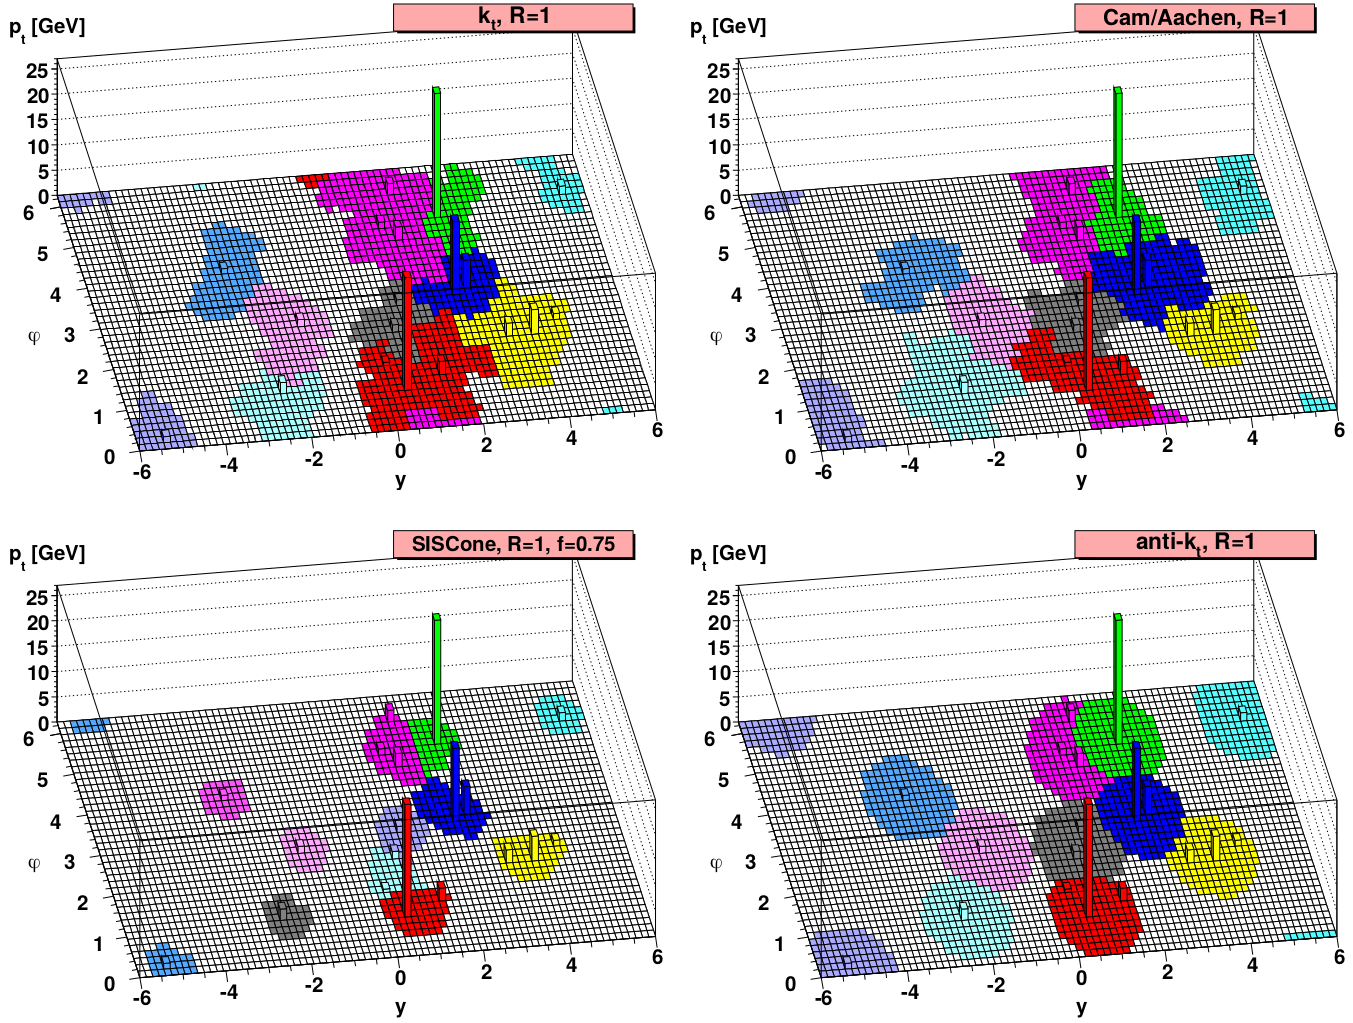
\includegraphics[width=.8\textwidth]{\PhDthesisdir/contents/chapter-JERC/reconstruction_des_jets/forme_des_jets.png}
\caption{Formes des jets reconstruits à partir de différents algorithmes pour un même événement~\cite{Cacciari_antikT}. En haut à gauche, \kT; en haut à droite, C/A; en bas à gauche, \textsc{SISCone}; en bas à droite, anti-\kT. L'algorithme anti-\kT\ permet d'obtenir des jets de forme régulière, conique.}
\label{fig-chapter-JERC-section-jets_reco-subsec-algo-examples}
\end{figure}
\par Le temps de calcul de ces algorithmes est un enjeu majeur au LHC.
Leurs temps d'exécution sont représentés en fonction du nombre d'événements d'empilement sur la figure~\ref{fig-chapter-JERC-section-jets_reco-subsec-algo-perfs}.
L'algorithme anti-\kT\ se place parmi les algorithmes les plus rapides.
Dans les conditions des collisions proton-proton du LHC, il permet le traitement d'un événement en moins d'une milliseconde.
C'est cet algorithme de regroupement qui est utilisé dans le cadre de l'expérience CMS.
\begin{figure}[h]
\centering
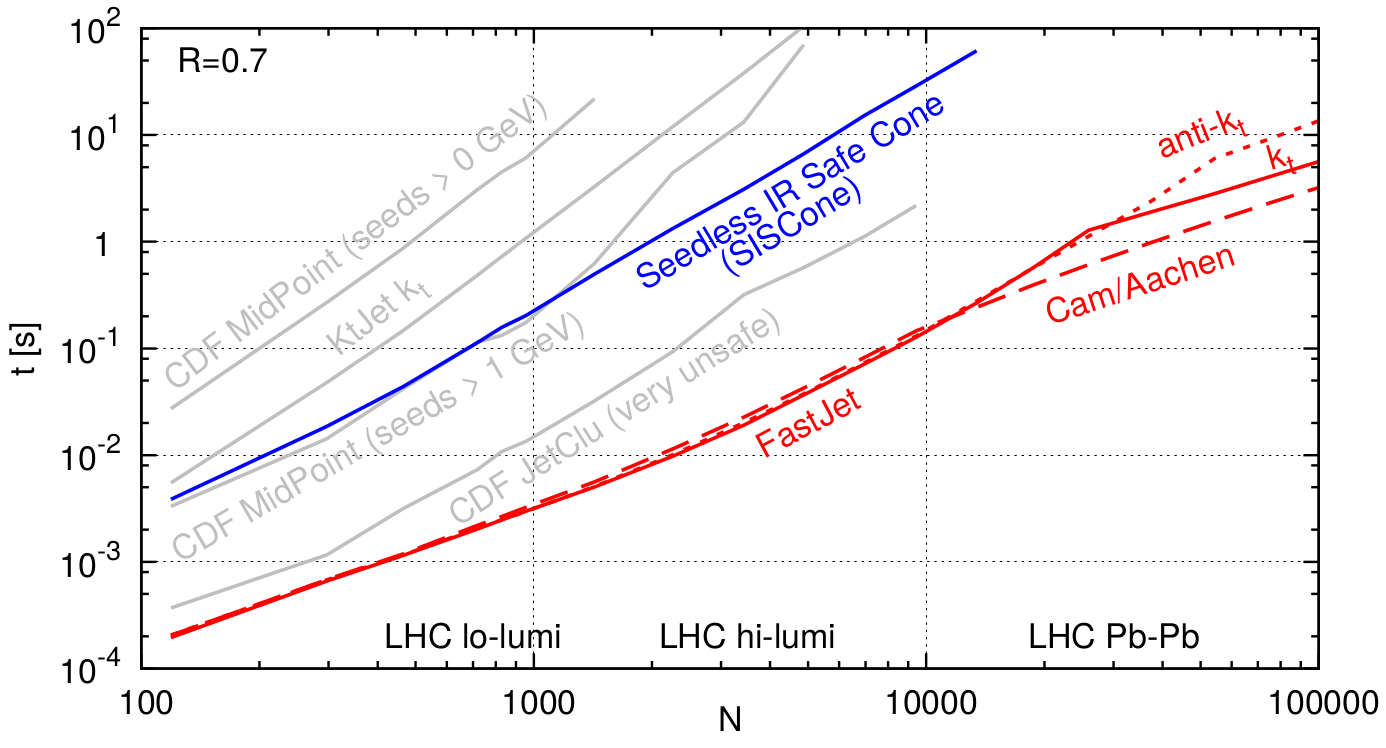
\includegraphics[width=.6\textwidth]{\PhDthesisdir/contents/chapter-JERC/reconstruction_des_jets/temps_de_calcul.png}
\caption{Temps de reconstruction d'un empilement d'un événement di-jets avec $N$ événements ne produisant que des jets de bas \pT\ pour différents algorithmes de reconstruction des jets.} % 50 GeV
\label{fig-chapter-JERC-section-jets_reco-subsec-algo-perfs}
\end{figure}
\subsection{Identification des jets dans CMS}\label{chapter-JERC-section-jets_reco-subsec-jetID}
Les jets ainsi reconstruits à l'aide des algorithmes de recombinaison sont en fait des \og candidats \fg{} jets.
À l'instar des particules individuelles, des critères d'identification leur sont appliqués afin de rejeter le bruit de fond et s'assurer de la qualité des jets ainsi reconstruits.
\par Ces critères reposent sur les caractéristiques des candidats jets comme la fraction d'énergie provenant de leurs constituants neutres ou encore le nombre de ces constituants.
Ces critères dépendent des années de prise de données et de la pseudo-rapidité du jet, \ie\ de la région du détecteur dans laquelle il se trouve.
\par Les critères utilisés pour les années 2016, 2017 et 2018, listés page~\pageref{tab-chapter-JERC-section-jets_reco-subsec-jetID-2017UL}, permettent d'obtenir une efficacité d'identification des jets supérieure à \SI{99}{\%} dans chacune des régions en $\eta$ du détecteur.
La réjection du bruit de fond est supérieure à \SI{98}{\%} pour $\abs{\eta}\leq\num{3.0}$ et supérieure à \SI{36}{\%} pour $\abs{\eta}>\num{3.0}$.
\begin{table}[p]
\centering
\begin{tabularx}{\textwidth}{lcYcY}
\toprule
Propriété du jet à identifier & $\abs{\eta}\leq\num{2.4}$ & $\num{2.4}<\abs{\eta}\leq\num{2.7}$ & $\num{2.7}<\abs{\eta}\leq\num{3.0}$ & $\num{3.0}<\abs{\eta}$ \\
\midrule
Fraction d'énergie\\
\labelitemi\ hadronique neutre & $<\num{0.90}$ & $<\num{0.90}$ & $<\num{0.98}$ & \\
\labelitemi\ électromagnétique neutre & $<\num{0.90}$ & $<\num{0.90}$ & $>\num{0.01}$ & $<\num{0.90}$ \\
\labelitemi\ hadronique chargée & $>\num{0}$ &&&\\
\labelitemi\ électromagnétique chargée & $<\num{0.99}$ &&&\\
\midrule
Nombre de constituants\\
\labelitemi\ neutres & $>\num{1}$ & $>\num{1}$ & $>\num{2}$ & $>\num{10}$ \\
\labelitemi\ chargés & $>\num{0}$ &&&\\
\bottomrule
\end{tabularx}

\caption{Critères d'identification des jets à CMS pour l'analyse des données de 2016.}
\label{tab-chapter-JERC-section-jets_reco-subsec-jetID-2016}
\end{table}
\begin{table}[p]
\centering
\begin{tabularx}{\textwidth}{lcYcY}
\toprule
Propriété du jet à identifier & $\abs{\eta}\leq\num{2.4}$ & $\num{2.4}<\abs{\eta}\leq\num{2.7}$ & $\num{2.7}<\abs{\eta}\leq\num{3.0}$ & $\num{3.0}<\abs{\eta}$ \\
\midrule
Fraction d'énergie\\
\labelitemi\ hadronique neutre & $<\num{0.90}$ & $<\num{0.90}$ &  & $>\num{0.02}$ \\
\labelitemi\ électromagnétique neutre & $<\num{0.90}$ & $<\num{0.90}$ & $<\num{0.99}$ et $>\num{0.02}$ & $<\num{0.90}$ \\
\labelitemi\ hadronique chargée & $>\num{0}$ &&&\\
\labelitemi\ électromagnétique chargée & $<\num{0.8}$ \\
\labelitemi\ muonique & $<\num{0.8}$ & $<\num{0.8}$ \\
\midrule
Nombre de constituants & $>\num{1}$ & $>\num{1}$\\
\labelitemi\ neutres & & & $>\num{2}$ & $>\num{10}$ \\
\labelitemi\ chargés & $>\num{0}$ &&&\\
\bottomrule
\end{tabularx}

\caption{Critères d'identification des jets à CMS pour l'analyse des données de 2017.}
\label{tab-chapter-JERC-section-jets_reco-subsec-jetID-2017}
\end{table}
\begin{table}[p]
\centering
\begin{tabularx}{\textwidth}{lcYcY}
\toprule
Propriété du jet à identifier & $\abs{\eta}\leq\num{2.6}$ & $\num{2.6}<\abs{\eta}\leq\num{2.7}$ & $\num{2.7}<\abs{\eta}\leq\num{3.0}$ & $\num{3.0}<\abs{\eta}\leq\num{5.0}$ \\
\midrule
Fraction d'énergie\\
\labelitemi\ hadronique neutre & $<\num{0.90}$ & $<\num{0.90}$ &  & $>\num{0.2}$ \\
\labelitemi\ électromagnétique neutre & $<\num{0.90}$ & $<\num{0.99}$ & $<\num{0.99}$ et $>\num{0.02}$ & $<\num{0.90}$ \\
\labelitemi\ hadronique chargée & $>\num{0}$ &&&\\
\midrule
Nombre de constituants & $>\num{1}$\\
\labelitemi\ neutres & & & $>\num{2}$ & $>\num{10}$ \\
\labelitemi\ chargés & $>\num{0}$ & $>\num{0}$ &&\\
\bottomrule
\end{tabularx}

\caption{Critères d'identification des jets à CMS pour l'analyse des données de 2018.}
\label{tab-chapter-JERC-section-jets_reco-subsec-jetID-2018}
\end{table}
\begin{table}[p]
\centering
\begin{tabularx}{\textwidth}{lcYcY}
\toprule
Propriété du jet à identifier & $\abs{\eta}\leq\num{2.6}$ & $\num{2.6}<\abs{\eta}\leq\num{2.7}$ & $\num{2.7}<\abs{\eta}\leq\num{3.0}$ & $\num{3.0}<\abs{\eta}\leq\num{5.0}$ \\
\midrule
Fraction d'énergie\\
\labelitemi\ hadronique neutre & $<\num{0.90}$ & $<\num{0.90}$ &  & $>\num{0.2}$ \\
\labelitemi\ électromagnétique neutre & $<\num{0.90}$ & $<\num{0.99}$ & $<\num{0.99}$ et $>\num{0.01}$ & $<\num{0.90}$ \\
\labelitemi\ hadronique chargée & $>\num{0}$ &&&\\
\labelitemi\ électromagnétique chargée & $<\num{0.8}$ & $<\num{0.8}$ \\
\labelitemi\ muonique & $<\num{0.8}$ & $<\num{0.8}$ \\
\midrule
Nombre de constituants & $>\num{1}$\\
\labelitemi\ neutres & & & $>\num{1}$ & $>\num{10}$ \\
\labelitemi\ chargés & $>\num{0}$ & $>\num{0}$ &&\\
\bottomrule
\end{tabularx}

\caption{Critères d'identification des jets à CMS pour l'analyse des données de 2017-UL.}
\label{tab-chapter-JERC-section-jets_reco-subsec-jetID-2017UL}
\end{table}
\subsection{Saveur des jets}\label{chapter-JERC-section-jets_reco-subsec-flavor}
b-tagging

\begin{figure}
\centering
\begin{tikzpicture}[scale=1.5]
\def\trackerrin{.100}
\def\trackerrout{1.185}
\def\trackercolor{ltcolorgray1}

\def\ECALrin{1.290}
\def\ECALrout{1.811}
\def\ECALcolor{ltcolorgreen1}

\def\HCALrin{1.812}
\def\HCALrout{2.854}
\def\HCALcolor{ltcoloryellow3}

\def\Solenrin{2.950}
\def\Solenrout{3.800}
\def\Solencolor{ltcolorgray2}

\def\ironryrina{3.850}
\def\ironryrouta{4.000}
\def\muonrina{4.020}
\def\muonrouta{4.400}
\def\ironryrinb{4.420}
\def\ironryroutb{4.880}
\def\muonrinb{4.905}
\def\muonroutb{5.285}
\def\ironryrinc{5.300}
\def\ironryroutc{5.960}
\def\muonrinc{5.975}
\def\muonroutc{6.355}
\def\ironryrind{6.375}
\def\ironryroutd{6.980}
\def\muonrind{7.000}
\def\muonroutd{7.380}
\def\muoncolor{ltcoloryellow1}
\def\ironrycolor{ltcolorred2}

\def\printele#1{
\draw [thick, ltcolorred] (0,0) arc (#1-90:#1-90+27:3) coordinate (eledeposit);
\draw [ltcolorred] (#1-5:1.25) node {\ele};
}
\def\printmu#1{
\draw [thick, ltcolorblue] (0,0) arc (#1-90:#1-90+33:6) arc (#1-90+33:#1-90:-12) node{\mu};
\draw [ltcolorblue] (#1-7:1.5) node {\mu};
}

\def\printantiele#1{
\draw [thick, ltcolorred] (0,0) arc (#1-90:#1-90-27:-3) coordinate (eledeposit);
\draw [ltcolorred] (#1-7:1.5) node {\ele};
%\draw [ltcolorred4, ultra thick] (eledeposit)--+(#1+25:\ECALrout);
}
\def\printantimu#1{
\draw [thick, ltcolorblue] (0,0) arc (#1-90:#1-90-33:-6) arc (#1-90-33:#1-90:12);
\draw [ltcolorblue] (#1-7:1.5) node {\mu};
}

\def\printtauh#1{
\draw [thick, ltcolorgreen4] (0,0) arc (#1-90:#1-90+11:10) ;
\draw [thick, ltcolorgreen4] (0,0) arc (#1-90:#1-90+6:20) ;
\draw [thick, ltcolorgreen4] (0,0) arc (#1-90:#1-90-11:-10) ;
\draw [ltcolorgreen4] (#1-12:1.5) node {\tauh};
}
\def\printantitauh#1{
\draw [thick, ltcolorgreen4] (0,0) arc (#1-90:#1-90-11:-10) ;
\draw [thick, ltcolorgreen4] (0,0) arc (#1-90:#1-90-6:-20) ;
\draw [thick, ltcolorgreen4] (0,0) arc (#1-90:#1-90+11:10) ;
\draw [ltcolorgreen4] (#1-12:1.5) node {\tauh};
}

\def\printjetnolabel#1{
\draw [thick, ltcolororange] (0,0) arc (#1-90+10:#1-90+22+10:5) ;
\draw [thick, ltcolororange] (0,0) arc (#1-90+5:#1-90+12+5:10) ;
\draw [thick, ltcolororange] (0,0) arc (#1-90:#1-90-22:-5) ;
\draw [thick, ltcolororange] (0,0) arc (#1-90:#1-90+6:20) ;
\draw [thick, ltcolororange] (0,0) arc (#1-90+5:#1-90+8+5:10) ;
\draw [thick, ltcolororange] (0,0) arc (#1-90:#1-90-11:-10) ;
\draw [thick, ltcolororange] (0,0) arc (#1-90:#1-90+11:10) ;
}

\def\printjet#1{
\printjetnolabel{#1}
\draw [ltcolororange] (#1-25:.5) node {jet};
}

\def\printjetfake#1{
\printjet{#1}
\draw [thick, ltcolorgreen4] (0,0) arc (#1-90:#1-90+11:10) ;
\draw [thick, ltcolorgreen4] (0,0) arc (#1-90:#1-90+6:20) ;
\draw [thick, ltcolorgreen4] (0,0) arc (#1-90:#1-90-11:-10) ;
\draw [ltcolorgreen4] (#1-17:1.5) node {f.\tauh};
}

\def\printdeposit#1#2#3#4{
\fill [#1] (#2-2:#3) arc (#2-2:#2+2:#3) -- (#2+2:#4) arc (#2+2:#2-2:#4) ;
}

\def\printECALdeposit#1#2{\printdeposit{#1}{#2}{\ECALrin}{\ECALrout}}
\def\printHCALdeposit#1#2{\printdeposit{#1}{#2}{\HCALrin}{\HCALrout}}

\def\printtauhdeposit#1{
\printHCALdeposit{ltcoloryellow4}{#1+3}
\printHCALdeposit{ltcoloryellow4}{#1+5}
\printHCALdeposit{ltcoloryellow4}{#1-5}
}

\def\printjetdeposit#1{
\printHCALdeposit{ltcoloryellow4}{#1+3}
\printHCALdeposit{ltcoloryellow4}{#1+5}
\printHCALdeposit{ltcoloryellow4}{#1-5}
\printHCALdeposit{ltcoloryellow4}{#1+21}
\printHCALdeposit{ltcoloryellow4}{#1+11}
\printHCALdeposit{ltcoloryellow4}{#1-11}
}

\def\printMuChSigA#1#2{
\fill [red] (#1-7.5+20*#2:\muonrina) arc (#1-7.5+20*#2:#1+7.5+20*#2:\muonrina) -- (#1+7.5+20*#2:\muonrouta) arc (#1+7.5+20*#2:#1-7.5+20*#2:\muonrouta) ;
}
\def\printMuChSigB#1#2{
\fill [red] (#1-7.5+20*#2:\muonrinb) arc (#1-7.5+20*#2:#1+7.5+20*#2:\muonrinb) -- (#1+7.5+20*#2:\muonroutb) arc (#1+7.5+20*#2:#1-7.5+20*#2:\muonroutb) ;
}
\def\printMuChSigC#1#2{
\fill [red] (#1-7.5+20*#2:\muonrinc) arc (#1-7.5+20*#2:#1+7.5+20*#2:\muonrinc) -- (#1+7.5+20*#2:\muonroutc) arc (#1+7.5+20*#2:#1-7.5+20*#2:\muonroutc) ;
}
\def\printMuChSigD#1#2{
\fill [red] (#1-7.5+20*#2:\muonrind) arc (#1-7.5+20*#2:#1+7.5+20*#2:\muonrind) -- (#1+7.5+20*#2:\muonroutd) arc (#1+7.5+20*#2:#1-7.5+20*#2:\muonroutd) ;
}

\foreach\jetangle in {120,-145}{
\printbigjetnolabel{\jetangle}
\draw (\jetangle:2.5) node {jet} ;
}

\def\Bjetangle{30}
\def\Bhaddronangle{5}
\def\Bhaddronflight{.75}

\def\CurrentVertex{(\Bhaddronangle:\Bhaddronflight)}

\draw [thick, dotted] (0,0) -- \CurrentVertex ;

{
\def\jetcolor{ltcolorred}
\printjetnolabel{\Bjetangle}
\draw [\jetcolor] (\Bjetangle:2)+(1.5,.75) node {traces déplacées};
}
\begin{scope}
\clip circle (\Solenrin);
\printantimuonnolabel{\Bjetangle}
\end{scope}

\draw [\muoncolor] (\Bjetangle:4) +(0,{-2*\baselineskip}) node {lepton chargé};

\draw (\Bjetangle:4) + (-.125,-.5) circle (1.125);
\draw [-latex] (\Bjetangle:4) + (-.125,-1.625) --+ (-.125,-2) node [below] {jet de saveur lourde};

\draw (0,0) node [left] {PV} ;
\draw \CurrentVertex node [below right] {SV} ;

\fill (0,0) circle (2pt);
\fill \CurrentVertex circle (2pt);

\draw [dashed] \CurrentVertex --+ (\Bjetangle:-.8);

\draw [red, latex-latex] (0,0)--+ (-90+\Bjetangle:{\Bhaddronflight*sin(\Bjetangle-\Bhaddronangle)}) node [below right] {IP};
\end{tikzpicture}
\end{figure}

\section{Calibration en énergie des jets dans CMS}\label{chapter-JERC-section-CMS}
Les jets sont des objets physiques composites complexes qu'il est nécessaire de calibrer, comme tout autre objet reconstruit.
La précision apportée à la mesure des jets est capitale dans de nombreuses analyses, où il s'agit d'une source majeure d'incertitude systématique.
Les avancées réalisées récemment sur la calibration des jets ont ainsi permis d'améliorer la précision sur la mesure de la section efficace inclusive de production de jets et de la masse du quark top~\cite{JERC_RunI}.
\par À partir des jets reconstruits par les méthodes décrites précédemment, un procédé de correction de l'énergie des jets (JEC, \emph{Jet Energy Correction}) est réalisé.
Il permet de corriger l'échelle en énergie des jets (JES, \emph{Jet Energy Scale}) ainsi que la résolution sur cette énergie (JER, \emph{Jet Energy Resolution}).
La collaboration CMS utilise une approche factorisée dans laquelle plusieurs étapes corrigent chacune un effet en particulier et dépendent des étapes précédentes~\cite{JERC_RunI}.
La figure~\ref{fig-CMS-JME-13-004_Figure_002-TeX} résume ces étapes, décrites dans les sections qui suivent.
\begin{figure}[h]
\centering
\includegraphics[width=\textwidth]{\PhDthesisdir/plots_and_images/from_JERC_RunI/CMS-JME-13-004_Figure_002-FR-TeX.tex}
\caption[Étapes successives de la JEC.]{Étapes successives de la JEC pour les données et les simulations~\cite{JERC_RunI}. Les corrections des étapes marquées \og MC \fg{} sont obtenues par l'étude de simulations, celles marquées \og RC \fg{} par une méthode de cône aléatoire (\emph{Random Cone}) sur les données. Les types d'événements utilisés dans les corrections résiduelles sont également indiqués.}
\label{fig-CMS-JME-13-004_Figure_002-TeX}
\end{figure}
\par Trois stades ou \og niveaux \fg{} de correction sur les particules peuvent être définis.
\begin{itemize}
\item Le niveau \og particule \fg, noté \ptcl, ou niveau \og vrai \fg{}, se réfère aux objets et variables après hadronisation mais avant interaction avec le détecteur. Il s'agit donc des grandeurs recherchées, uniquement accessibles dans les événements simulés.
\item Le niveau \og reconstruit \fg, noté \reco, correspond aux objets et variables après interaction avec le détecteur et reconstruction par l'algorithme de \PF.
\item Le niveau \og corrigé \fg{} ou calibré, noté \cali, correspond aux objets et variables corrigés, \ie\ ceux du niveau reconstruit auxquels ont été appliquées les corrections.
\end{itemize}
La réponse d'un jet, variable importante pour ce chapitre, est définie comme
\begin{equation}
R = \frac{\pT}{\pT_\ptcl}
\mend
\end{equation}
La réponse peut être définie à différents niveaux, et par définition $R_\ptcl=1$.
Si la JEC est correcte, alors l'impulsion transverse du jet corrigé doit correspondre sensiblement à l'impulsion transverse au niveau particule, \ie\ $R_\cali\simeq1$.
Sur la figure~\ref{fig-JERC_RunI-1} sont représentées les réponses de jets d'événements QCD simulés à différentes étapes de la JEC. Après avoir appliqué toutes les corrections, ce qui correspond à la figure~\ref{subfig-JERC_RunI-1_3}, la réponse est sensiblement égale à 1, ce qui montre que la JEC est correcte.
\begin{figure}[h]
\centering
\subcaptionbox{Avant correction ($R_\reco$).\label{subfig-JERC_RunI-1_1}}[.3\textwidth]
{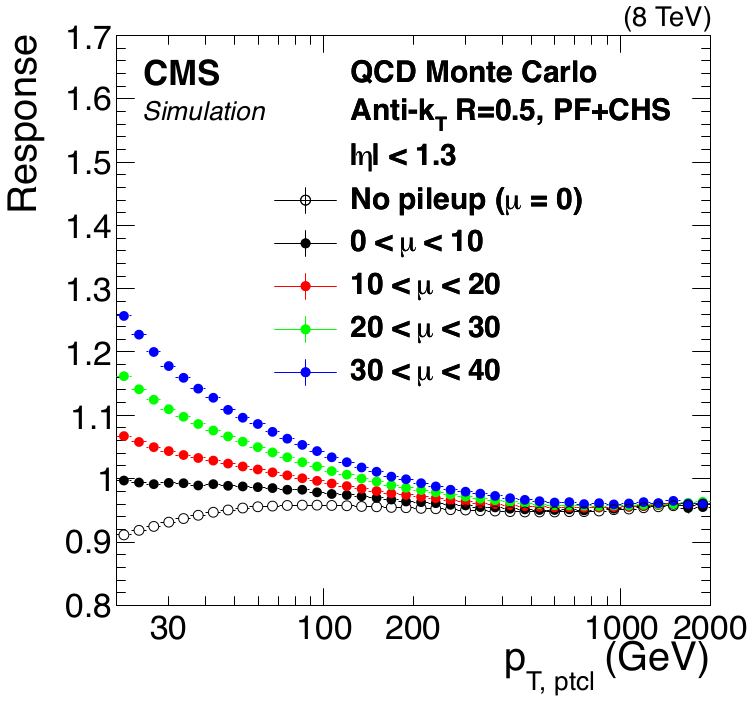
\includegraphics[width=.3\textwidth]{\PhDthesisdir/plots_and_images/from_JERC_RunI/response_evolution_1.png}}
\hfill
\subcaptionbox{Correction de l'empilement.\label{subfig-JERC_RunI-1_2}}[.3\textwidth]
{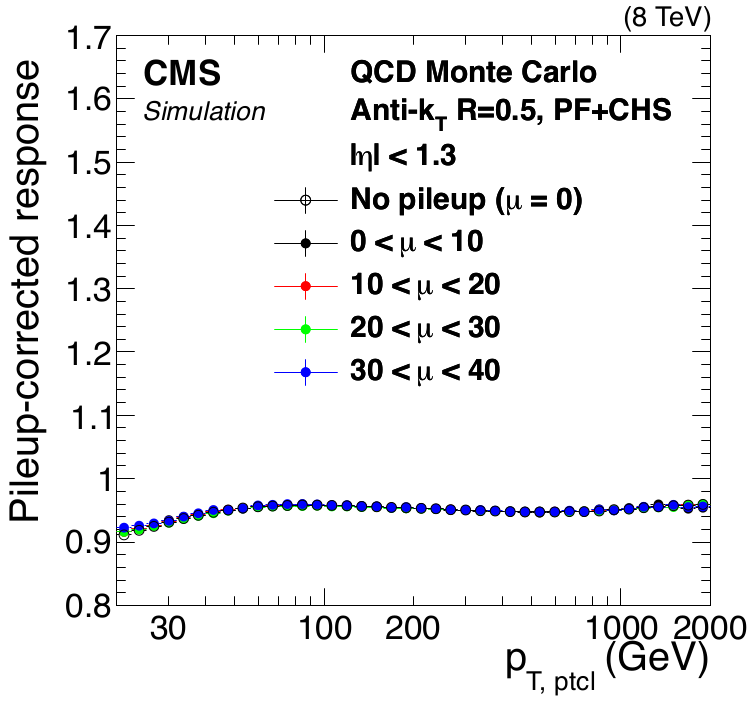
\includegraphics[width=.3\textwidth]{\PhDthesisdir/plots_and_images/from_JERC_RunI/response_evolution_2.png}}
\hfill
\subcaptionbox{Après correction ($R_\cali$).\label{subfig-JERC_RunI-1_3}}[.3\textwidth]
{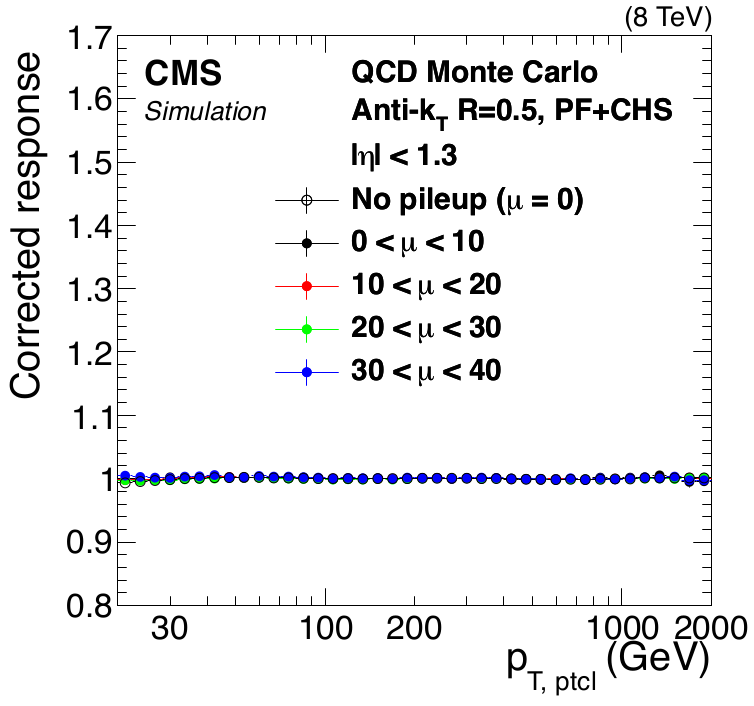
\includegraphics[width=.3\textwidth]{\PhDthesisdir/plots_and_images/from_JERC_RunI/response_evolution_3.png}}
\caption[Valeur moyenne de la réponse de jets d'événements QCD simulés.]{Valeur moyenne de la réponse de jets d'événements QCD simulés en fonction de $\pT_\ptcl$ à différentes étapes de la JEC~\cite{JERC_RunI} et pour différentes valeurs d'interactions d'empilement $\mu$.}
\label{fig-JERC_RunI-1}
\end{figure}
\par Les jets au niveau particule sont reconstruits en appliquant la procédure de recombinaison à toutes les particules de durée de vie $\tau$ telle que $c\tau>\SI{1}{\centi\meter}$ à l'exception des neutrinos~\cite{JERC_RunI}.
Les hadrons contenant des quarks~\quarkc\ ou~\quarkb\ ne rentrent pas dans cette catégorie et ce sont donc leurs produits de désintégration qui sont pris en compte pour la recombinaison.
Les neutrinos sont exclus pour pouvoir définir la réponse des jets d'une manière qui soit accessible expérimentalement et qui réduise significativement les différences de réponse entre jets lourds et jets légers ou de gluons, à cause des neutrinos produits dans les désintégration des quarks lourds.
\subsection{Correction de l'empilement}\label{chapter-JERC-section-CMS-subsec-PU}
Des contributions additionnelles à l'énergie et à l'impulsion des jets peuvent apparaître du fait de l'empilement, décrit dans la section~\ifref{chapter-LHC-section-LHC-subsec-PU}{\ref{chapter-LHC-section-LHC-subsec-PU}}{1.4} du chapitre~\ifref{chapter-LHC}{\ref{chapter-LHC}}{3}.
La correction de l'empilement a pour but de soustraire ces contributions et est appliquée dans les données et les événements simulés.
Elle permet d'améliorer la résolution en énergie des jets et d'obtenir une JES plus précise.
\par L'empilement asynchrone est réduit par l'analyse temporelle des signaux des calorimètres,
l'empilement synchrone par la méthode de soustraction des hadrons chargés (CHS, \emph{pile-up Charged Hadron Subtraction}), décrite ci-après.
\par Pour chacun des vertex primaires de l'événement, la somme des impulsions transverses au carré des traces associées au vertex est calculée.
Le vertex primaire principal est choisi comme étant le vertex présentant la plus grande valeur de cette somme.
Les autres vertex primaires sont considérés comme des vertex d'empilement.
Les hadrons chargés dont les traces associées proviennent de vertex d'empilement sont retirés de l'événement.
La reconstruction des jets est alors réalisée à partir de l'événement nettoyé, ce qui permet d'améliorer la résolution en \pT\ des jets.
\par La correction de l'empilement résiduel, principalement due aux hadrons neutres, aux photons, aux traces non associées à un vertex et à l'empilement asynchrone qui n'a pas pu être corrigé totalement, est déterminée à l'aide de la méthode de l'aire hybride (\emph{hybrid jet area}).
Il s'agit d'une correction paramétrique, appliquée indépendamment à chaque jet, dépendante de:
\begin{itemize}
\item la densité en énergie dans le plan $(\eta, \phi)$ de l'événement contenant ce jet, notée $\rho$;
\item l'aire du jet dans le plan $(\eta, \phi)$, $A_j$;
\item la pseudo-rapidité du jet, $\eta$;
\item l'impulsion transverse du jet avant application de cette correction et après CHS, $\pT_\reco^\text{CHS}$.
\end{itemize}
La correction $\mathcal{C}_\text{PU}$ à appliquer à un jet s'exprime alors
\begin{equation}
\mathcal{C}_\text{PU}(\pT_\reco^\text{CHS}, \eta, A_j, \rho)
= 1 - \frac{\left[\rho_0(\eta) + \rho\,\beta(\eta)(1+\gamma(\eta)\log\pT_\reco^\text{CHS})\right]A_j}{\pT_\reco^\text{CHS}}
\label{eq-chapter-JERC-section-CMS-subsec-PU-offset_corr_v1}
\end{equation}
où $\rho_0(\eta)$, $\beta(\eta)$ et $\gamma(\eta)$ sont les paramètres de cette correction, dépendants de $\eta$.
Ils sont déterminés à partir de la contribution additionnelle de l'empilement au niveau particule $\pT_\ptcl^\text{add}$, estimée à partir d'événements QCD multijet simulés avec et sans empilement, telle que
\begin{equation}
\average{\pT_\ptcl^\text{add}}(\rho, \eta, \pT_\reco^\text{CHS})
=
\average{\pT_\ptcl^\text{avec PU} - \pT_\ptcl^\text{sans PU}}
\mend[,]
\label{eq-chapter-JERC-section-CMS-subsec-PU-pTaddptcl}
\end{equation}
avec
$\pT_\ptcl^\text{avec PU}$ et $\pT_\ptcl^\text{sans PU}$
les impulsions du jet au niveau particule avec et sans empilement.
La contribution additionnelle de l'empilement au niveau particule est alors paramétrée en fonction de $\rho$, $\eta$, $\pT_\reco^\text{CHS}$ et $A_j$ afin d'obtenir les paramètres $\rho_0(\eta)$, $\beta(\eta)$ et $\gamma(\eta)$ de l'équation~\eqref{eq-chapter-JERC-section-CMS-subsec-PU-offset_corr_v1} qui peut se réécrire
\begin{equation}
\mathcal{C}_\text{PU}(\pT_\reco^\text{CHS}, \eta, A_j, \rho)
= 1 - \frac{\average{\pT_\ptcl^\text{add}}}{\pT_\reco^\text{CHS}}
\mend
\label{eq-chapter-JERC-section-CMS-subsec-PU-offset_corr_v2}
\end{equation}
La figure~\ref{fig-chapter-JERC-section-CMS-subsec-PU-JERC_RunI-Figure_005} montre $\average{\pT_\ptcl^\text{add}}$ en fonction de l'impulsion transverse du jet au niveau particule, avant et après application de la correction de l'empilement.
Les résultats de la figure~\ref{subfig-chapter-JERC-section-CMS-subsec-PU-JERC_RunI-Figure_005b} sont cohérents avec l'absence d'énergie supplémentaire due à l'empilement à $\pm\SI{0.2}{\GeV}$. Dans le cas d'un grand nombre d'interactions d'empilement ($\mu>30$), un léger effet est visible, lié à une dépendance quadratique en $\rho$ de la contribution en énergie de l'empilement qui n'est pas modélisée~\cite{JERC_RunI}.
\begin{figure}[h]
\centering
\subcaptionbox{Avant correction.\label{subfig-chapter-JERC-section-CMS-subsec-PU-JERC_RunI-Figure_005a}}[.45\textwidth]
{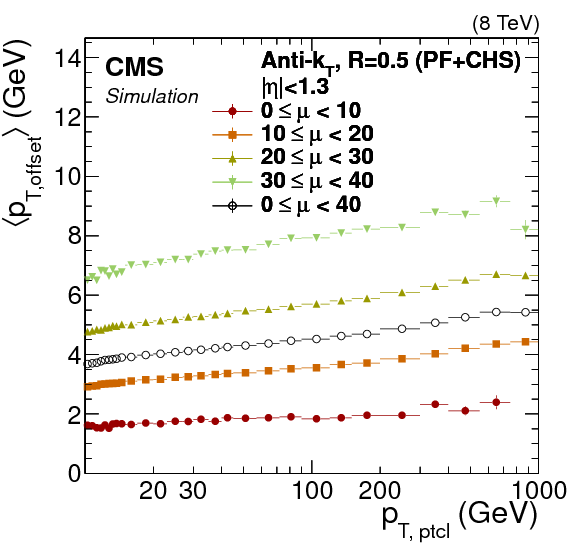
\includegraphics[width=.45\textwidth]{\PhDthesisdir/plots_and_images/from_JERC_RunI/Figure_005-a.tex}}
\hfill
\subcaptionbox{Après correction.\label{subfig-chapter-JERC-section-CMS-subsec-PU-JERC_RunI-Figure_005b}}[.45\textwidth]
{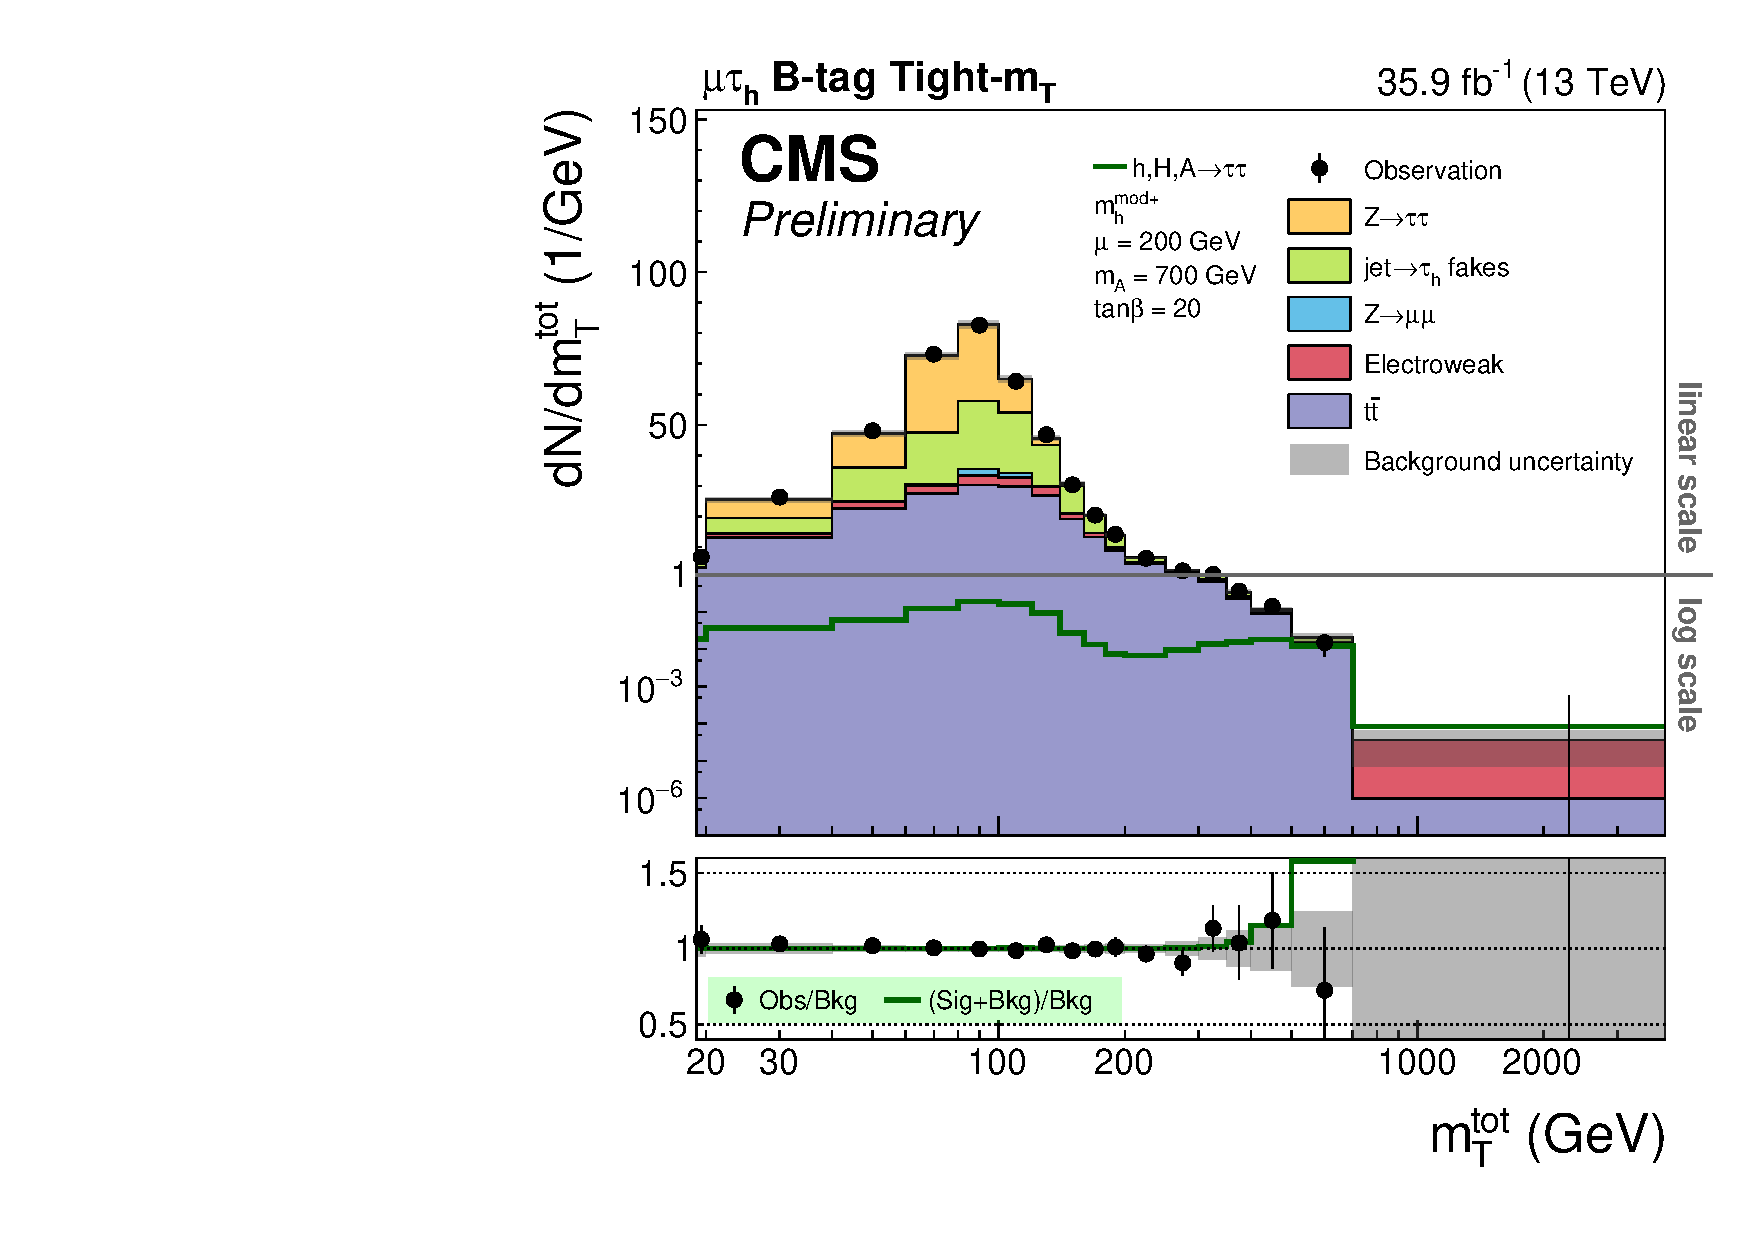
\includegraphics[width=.45\textwidth]{\PhDthesisdir/plots_and_images/from_JERC_RunI/Figure_005-b.tex}}
\caption[Contribution additionnelle de l'empilement au niveau particule.]{Contribution additionnelle de l'empilement au niveau particule telle que définie dans l'équation~\eqref{eq-chapter-JERC-section-CMS-subsec-PU-pTaddptcl} pour $\abs{\eta}<\num{1.3}$ en fonction de l'impulsion du jet au niveau particule pour différentes valeurs du nombre d'interaction d'empilement ($\mu$)~\cite{JERC_RunI}.}
\label{fig-chapter-JERC-section-CMS-subsec-PU-JERC_RunI-Figure_005}
\end{figure}
\par La correction ainsi décrite doit être légèrement adaptée pour pouvoir l'appliquer aux données à cause des biais de simulation du détecteur.
Pour cela, un ajustement en fonction de $\eta$ est déterminé à l'aide de la méthode de cône aléatoire (RC, \emph {Random Cone}). La méthode RC reconstruit les jets à l'aide de cônes dont la direction en $(\eta, \phi)$ est choisie de manière aléatoire.
L'étude est réalisée sur des événements dits de \og zéro biais \fg.
Il s'agit d'événements sélectionnés par un déclenchement aléatoire pendant que les faisceaux de protons se croisent.
Le déclenchement n'étant pas dû à un dépôt d'énergie en particulier, ces événements ne comportent pas, en général, de contribution provenant d'une interaction dure, \ie\ d'une collision effective entre les protons.
Dans ce cas, la valeur moyenne de l'impulsion transverse des jets reconstruits par la méthode RC permet d'estimer la moyenne de la contribution additionnelle de l'empilement, \ie
\begin{equation}
\average{\pT^\text{add}}^\text{RC} = \average{\pT_\text{cône}}
\mend
\end{equation}
Il est alors possible de définir un facteur d'échelle à appliquer aux paramètres $\rho_0$ et $\beta$ de l'équation~\eqref{eq-chapter-JERC-section-CMS-subsec-PU-offset_corr_v1} lorsque cette correction est appliquée aux données. Ce facteur d'échelle s'exprime
\begin{equation}
\frac{\average{\pT^\text{add}}^\text{RC}_\text{données}(\eta, \rho_\text{données})}{\average{\pT^\text{add}}^\text{RC}_\text{simulation}(\eta, \rho_\text{simulation})}
\mend
\end{equation}
La contribution additionnelle de l'empilement est ainsi corrigée dans les simulations et les données.
\subsection{Correction de la réponse du détecteur en $\pT$ et en $\eta$}\label{chapter-JERC-section-CMS-subsec-reponse}
La réponse du détecteur CMS à un jet n'est pas uniforme selon la valeur de \pT\ et $\eta$ du jet.
La réponse au niveau reconstruit de jets simulés $R_\reco$,
déterminée grâce à une simulation du détecteur CMS basée sur \GEANTfour~\cite{geant4_2003,geant4_2006,geant4_2016},
combinée à \PYTHIA~6.4~\cite{pythia6.4}
avec les réglages Z2*~\cite{tunes_2016},
est représentée sur la figure~\ref{fig-simulated_jet_response_RunII} pour les trois années du Run~II du LHC.
Il apparaît, par exemple, qu'un jet de $\pT=\SI{30}{\GeV}$ nécessite une correction allant de \SI{10}{\%} dans la région centrale $\abs{\eta}<\num{0.7}$ à plus de \SI{30}{\%} lorsque $\abs{\eta}\simeq\num{3}$ en 2017 et 2018.
\begin{figure}[h]
\centering
\subcaptionbox{Année 2016.\label{subfig-simulated_jet_response_2016}}[.3\textwidth]
{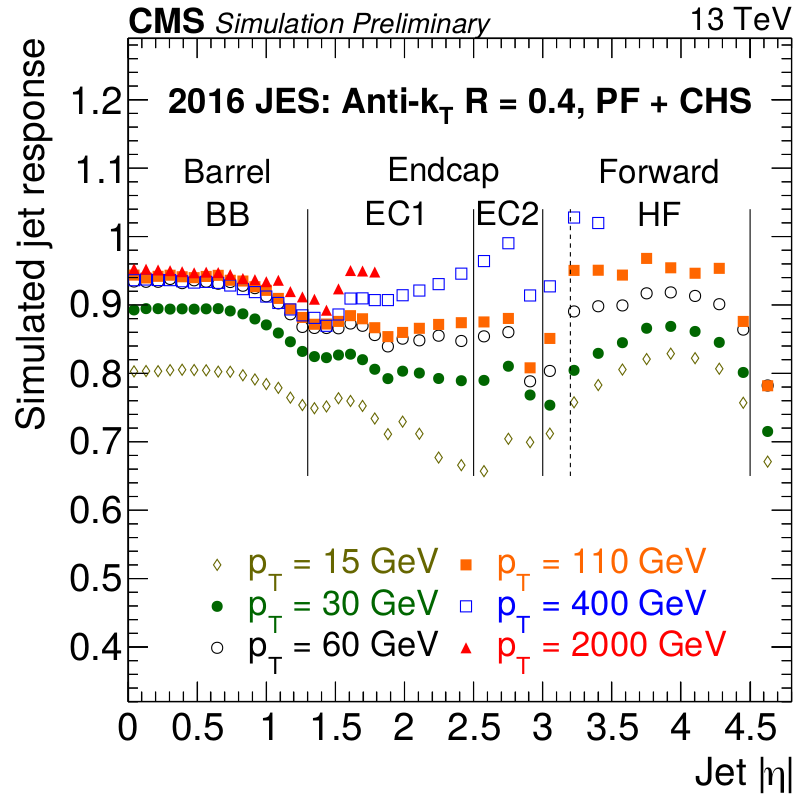
\includegraphics[width=.3\textwidth]{\PhDthesisdir/plots_and_images/from_CMS-DP-2020-019/simulated_jet_response_2016.png}}
\hfill
\subcaptionbox{Année 2017.\label{subfig-simulated_jet_response_2017}}[.3\textwidth]
{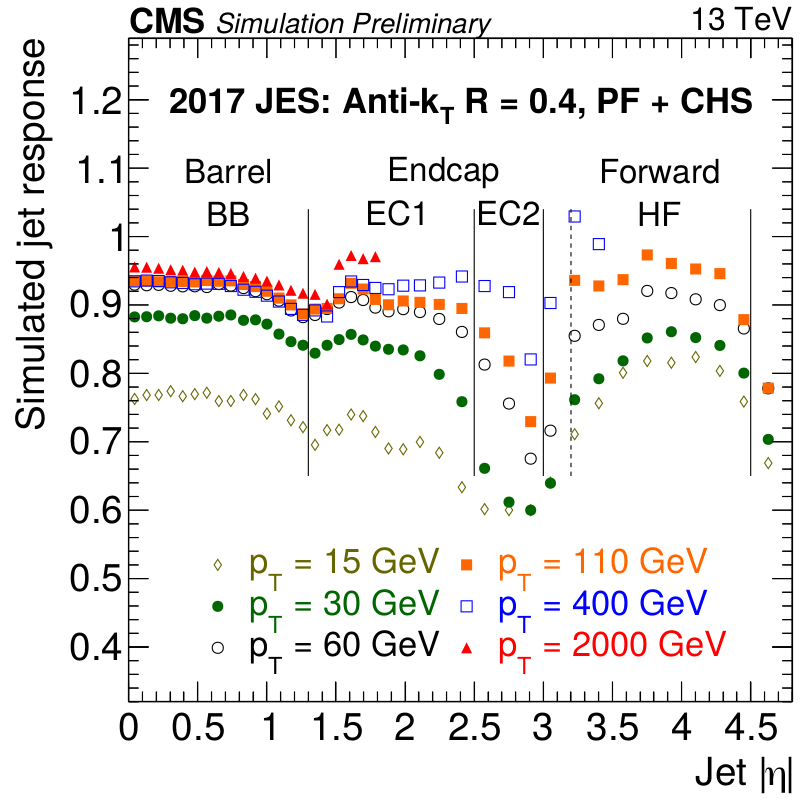
\includegraphics[width=.3\textwidth]{\PhDthesisdir/plots_and_images/from_CMS-DP-2020-019/simulated_jet_response_2017.png}}
\hfill
\subcaptionbox{Année 2018.\label{subfig-simulated_jet_response_2018}}[.3\textwidth]
{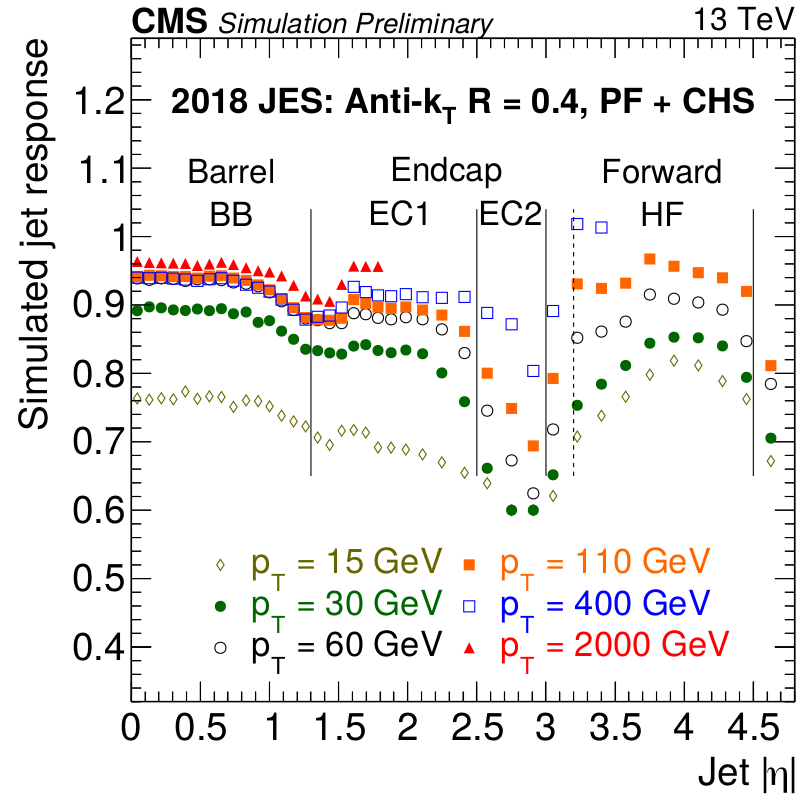
\includegraphics[width=.3\textwidth]{\PhDthesisdir/plots_and_images/from_CMS-DP-2020-019/simulated_jet_response_2018.png}}
\caption[Réponse des jets reconstruits en fonction de \pT\ et $\eta$ lors du Run~II.]{Réponse des jets reconstruits en fonction de \pT\ et $\eta$ lors du Run~II~\cite{CMS-DP-2020-019}. La chute de la réponse des jets dans la région $\abs{\eta}\simeq\num{3}$ est due à la transition entre le bouchon (\emph{Endcap}) et la partie avancée (\emph{Forward}) du détecteur. Pour $\abs{\eta}>\num{4.5}$, les limites du détecteur en termes d'acceptation expliquent la chute de la réponse des jets. La dégradation au cours du temps du détecteur dans la région \og EC2 \fg{} s'observe par la baisse de la réponse des jets dans cette région de 2016 à 2017.}
\label{fig-simulated_jet_response_RunII}
\end{figure}
\par Afin de corriger la réponse du détecteur en $\pT$ et en $\eta$, la correction $\mathcal{C}_\text{Rép}$ à appliquer s'exprime
\begin{equation}
\mathcal{C}_\text{Rép}(\pT_\reco', \eta) = \frac{\average{\pT_\ptcl}}{\average{\pT_\reco'}} = \frac{1}{\average{R_\reco'}}
\end{equation}
où $\pT_\reco'$ est l'impulsion transverse du jet après correction de l'empilement.
Les moyennes sont réalisées sur les jets appartenant à la même cellule d'une grille en $(\pT_\ptcl, \eta)$ prédéfinie~\cite{JERC_RunI}.
\subsection{Propagation à la MET}\label{chapter-JERC-section-CMS-subsec-MET}
L'impulsion transverse manquante \vMET\footnote{L'impulsion transverse manquante est définie dans la section~\ifref{chapter-LHC-section-evt_reco-subsec-MET}{\ref{chapter-LHC-section-evt_reco-subsec-MET}}{4.4} du chapitre\ifref{chapter-LHC}{~\ref{chapter-LHC}}{ \og Dispositif expérimental \fg}.} doit prendre en compte les corrections apportées aux jets afin de garder une description cohérente de l'événement.
La JEC est ainsi propagée à \vMET\ par la correction dite de \og type-I \fg,
\begin{equation}
\vMET_\text{type-I} = \vMET_\reco + \sum_{\substack{\text{jets}\\\pT_\reco>\SI{15}{\GeV}}} \left(\vpT_\reco - \vpT_\cali\right) - \vec{\mathcal{O}}_\text{RC}
\end{equation}
où $\vpT_\cali$ correspond à l'impulsion transverse du jet après correction de la réponse du détecteur
et
$\vec{\mathcal{O}}_\text{RC}$ la contribution moyenne de l'empilement obtenue par la méthode RC.
\subsection{Corrections résiduelles}\label{chapter-JERC-section-CMS-subsec-residuals}
Les corrections décrites dans les sections précédentes permettent d'obtenir une bonne correction en énergie des jets.
Toutefois, des différences dans les réponses des jets, de l'ordre du pourcent, subsistent entre données et simulations.
Des corrections résiduelles à appliquer aux données sont ainsi déterminées afin de réduire ces écarts, définies telles que
\begin{equation}
\mathcal{C}_\text{Res} = \frac{R_\text{simulations}}{R_\text{données}}
\mend
\label{eq-chapter-JERC-section-CMS-subsec-residuals-Cres_def}
\end{equation}
\par Le principe est d'estimer la réponse du jet en s'appuyant sur un objet de référence pouvant être un boson \Zboson\ (événements \Zjets), un photon (événements \Gjets) ou un autre jet (événements dijet et multijet).
Deux méthodes existent et sont utilisées de manière complémentaire:
\begin{description}
\item[la méthode de la balance] estime que l'objet de référence et le jet sont balancés au niveau particule, \ie\ d'impulsion transverse totale nulle, soit
\begin{equation}
\vpT_\ptcl^\text{réf} + \vpT_\ptcl^\text{jet} = \vec{0}
\Rightarrow
\pT_\ptcl^\text{jet} = \pT_\ptcl^\text{réf}
\mend
\end{equation}
Ainsi, au niveau reconstruit\footnote{Le niveau reconstruit prend ici en compte les étapes de correction de l'empilement et de la réponse du détecteur.},
\begin{equation}
\vpT_\reco^\text{réf} + \vpT_\reco^\text{jet} = \vec{0}
\Leftrightarrow
\vpT_\ptcl^\text{réf} + \Rbal\vpT_\ptcl^\text{jet} = \vec{0}
\end{equation}
car l'objet de référence, fidèlement reconstruit, permet de considérer
\begin{equation}
\vpT_\reco^\text{réf} \simeq \vpT_\ptcl^\text{réf} = \vpT^\text{réf}
\mend
\label{eq-chapter-JERC-section-CMS-subsec-residuals-pT_ref_approx_ptcl_reco}
\end{equation}
La réponse balancée \Rbal\ est alors définie comme
\begin{equation}
\Rbal (\pT, \eta) = \frac{\pT_\reco^\text{jet}}{\pT^\text{réf}}
\label{eq-chapter-JERC-section-CMS-subsec-residuals-Rbal_def}
\end{equation}
\item[la méthode \og MPF \fg] (\emph{MET Projection Fraction}) prend en compte l'ensemble de l'activité hadronique de l'événement et considère l'impulsion de recul vis-à-vis de l'objet de référence, \ie
\begin{equation}
\vpT_\ptcl^\text{réf} + \vpT_\ptcl^\text{recul} = \vec{0}
\Rightarrow
\vpT_\reco^\text{réf} + \vpT_\reco^\text{recul} = -\vMET
\Leftrightarrow
\vpT_\reco^\text{réf} + \RMPF\vpT_\ptcl^\text{recul} = -\vMET
\mend
\end{equation}
En appliquant~\eqref{eq-chapter-JERC-section-CMS-subsec-residuals-pT_ref_approx_ptcl_reco} à l'équation précédente, il est possible d'écrire
\begin{equation}
\vpT^\text{réf} - \RMPF\vpT^\text{réf} = -\vMET
\mend[,]
\end{equation}
ce qui permet de définir la réponse MPF \RMPF\ comme
\begin{equation}
\RMPF (\pT, \eta) = 1 + \frac{\vpT^\text{réf}\cdot\vMET}{\abs{\vpT^\text{réf}}^2}
\mend
\end{equation}
\end{description}
\subsubsection{Correction résiduelle relative en $\eta$}\label{chapter-JERC-section-CMS-subsec-residuals_eta}
La première de ces corrections résiduelles, fonction de $\eta$, est obtenue à partir de la comparaison données-simulations sur une sélection d'événements dijet.
Son but est de rendre indépendant de $\eta$ le rapport données sur simulations de la réponse des jets.
Cette correction s'appuie sur la bonne reconstruction des jets dans le barillet, c'est pourquoi elle est qualifiée de \og relative \fg.
\par Lorsqu'un événement présente un premier jet avec $\abs{\eta}<\num{1.3}$, \ie\ dans la région de référence du barillet, et un second avec $\abs{\eta}>\num{1.3}$ et de \pT\ similaire, le premier sert d'objet de référence afin de calibrer le second.
La correction à appliquer aux données ainsi obtenue est illustrée sur la figure~\ref{fig-L2ResRel_RunII} dans le cas des jets d'impulsion transverse égale à \SI{120}{\GeV}.
\begin{figure}[h]
\centering
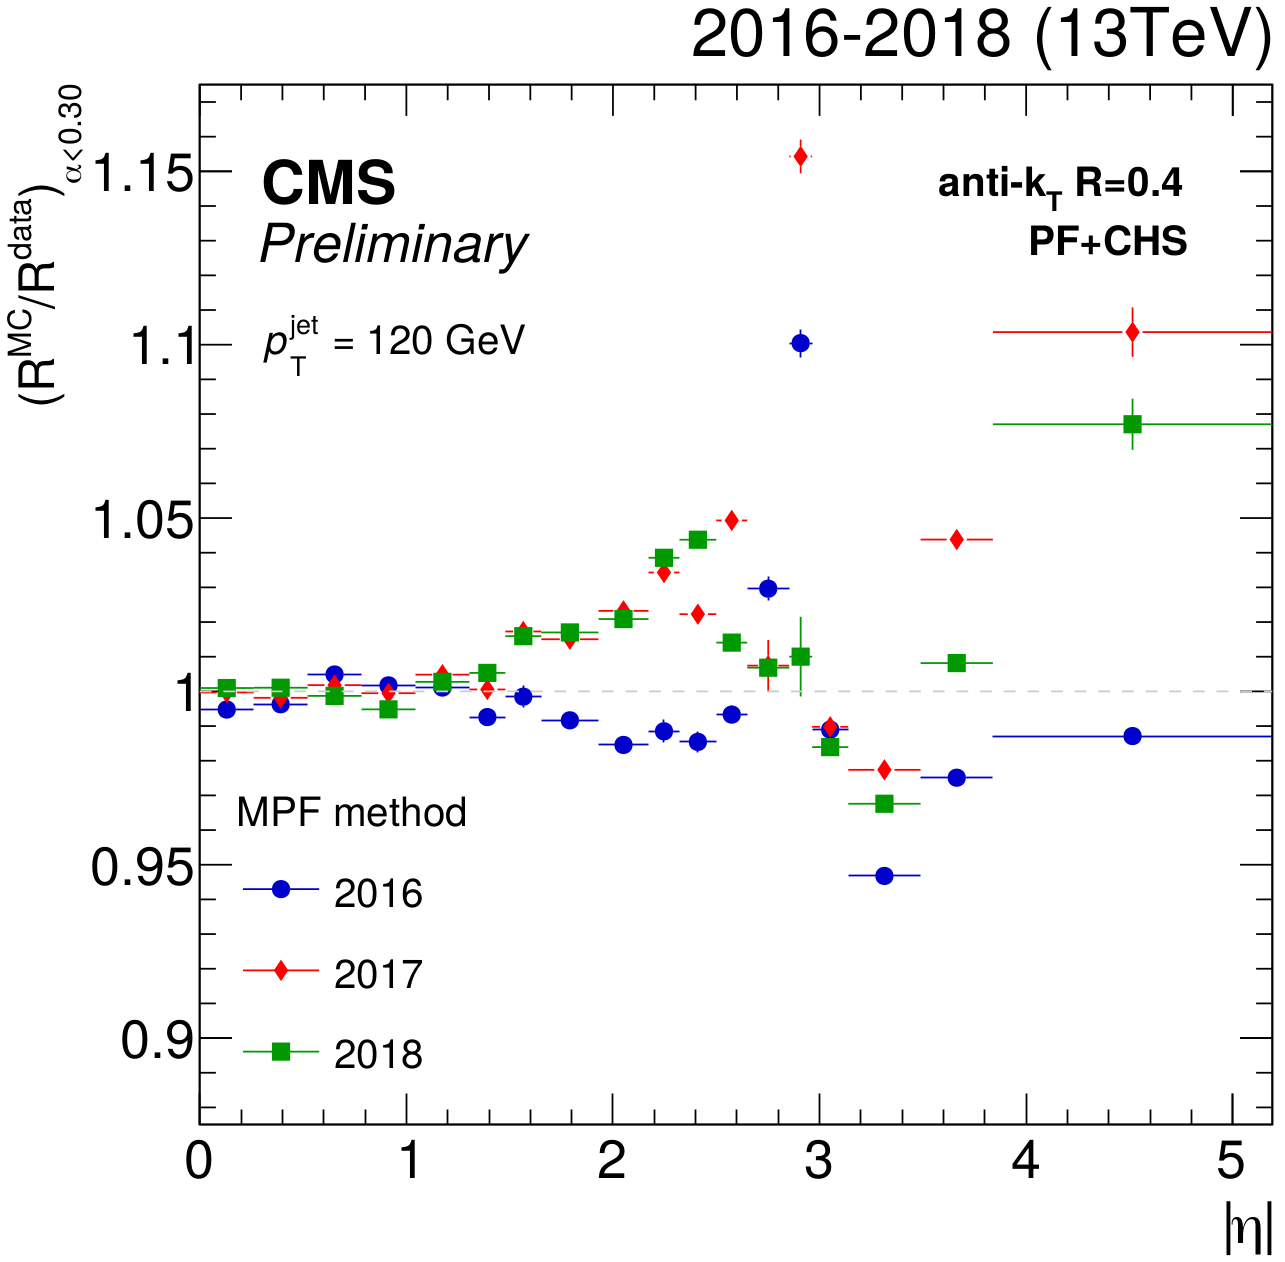
\includegraphics[width=.45\textwidth]{\PhDthesisdir/plots_and_images/from_CMS-DP-2020-019/relative_eta_residual_RunII.png}
\caption[Correction résiduelle relative en $\eta$ lors du Run~II.]{Correction résiduelle relative en $\eta$ lors du Run~II obtenue avec des événements dijet et la méthode MPF~\cite{CMS-DP-2020-019}.}
\label{fig-L2ResRel_RunII}
\end{figure}
\subsubsection{Correction résiduelle absolue en \pT}\label{chapter-JERC-section-CMS-subsec-residuals_pT}
Cette correction, fonction de \pT, a pour but de rendre indépendant de \pT\ le rapport données sur simulations de la réponse des jets.
Elle combine, à l'aide d'un ajustement global, les comparaisons données-simulations de plusieurs types d'événements afin de couvrir un large spectre de valeurs de \pT. Chaque type d'événement est en effet dominant, de par sa statistique, dans une gamme de \pT\ donnée:
\begin{itemize}
\item événements \Zjets: il s'agit d'événements \Zmmjets\ et \Zeejets, sélectionnés par la présence d'une paire de muons ou d'électrons compatibles avec la désintégration d'un \Zboson, ils couvrent la région $\pT<\SI{200}{\GeV}$;
\item événements \Gjets: sélectionnés dans les données à l'aide d'un déclenchement basé sur la présence d'un photon, ils permettent de traiter la région $\SI{200}{\GeV}<\pT<\SI{800}{\GeV}$;
\item événements multijet: ces événements contiennent au moins deux jets dans l'état final et couvrent la région $\pT>\SI{800}{\GeV}$.
\end{itemize}
En 2017 et 2018, les événements multijet n'ont pas été exploités et la correction résiduelle absolue en \pT\ dans la région $\pT>\SI{800}{\GeV}$ est contrainte par l'analyse des événements \Gjets.
\par L'objet de référence utilisé pour calibrer le jet, que ce soit un boson \Zboson\ (\Zjets), un photon (\Gjets) ou un autre jet (multijet), possède une meilleure résolution en énergie.
Cette correction corrige l'échelle en énergie absolue des jets, d'où son qualificatif. % d'\og absolue \fg.
La correction à appliquer aux données ainsi obtenue est illustrée sur la figure~\ref{fig-L3ResAbs_RunII} dans le cas des jets de pseudo-rapidité $\abs{\eta}<\num{1.3}$.
\begin{figure}[h]
\centering
\subcaptionbox{Année 2016.\label{subfig-absolute_pT_residual_2016}}[.3\textwidth]
{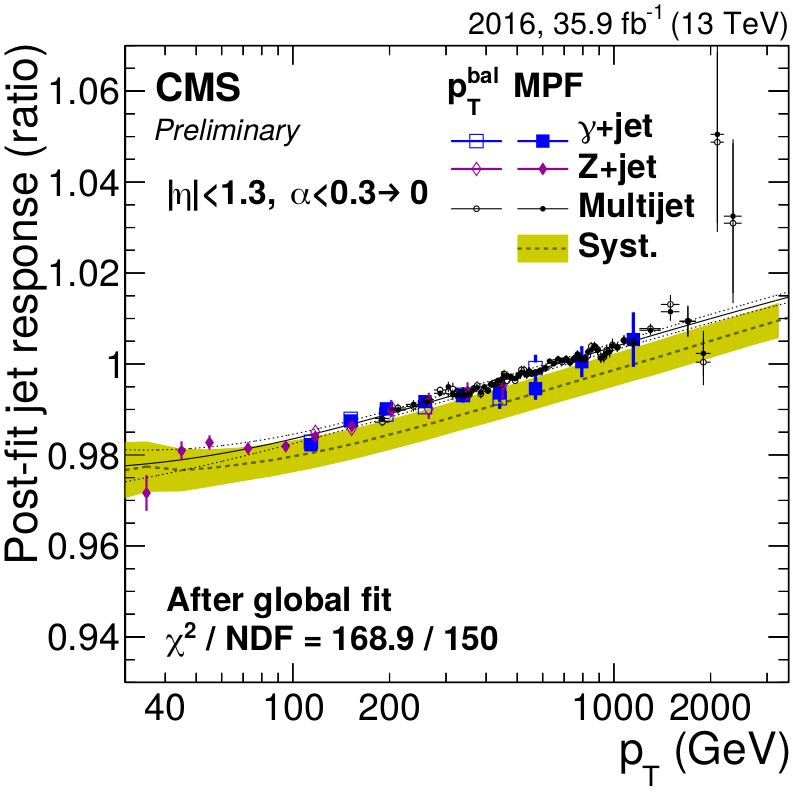
\includegraphics[width=.3\textwidth]{\PhDthesisdir/plots_and_images/from_CMS-DP-2020-019/absolute_pT_residual_2016.png}}
\hfill
\subcaptionbox{Année 2017.\label{subfig-absolute_pT_residual_2017}}[.3\textwidth]
{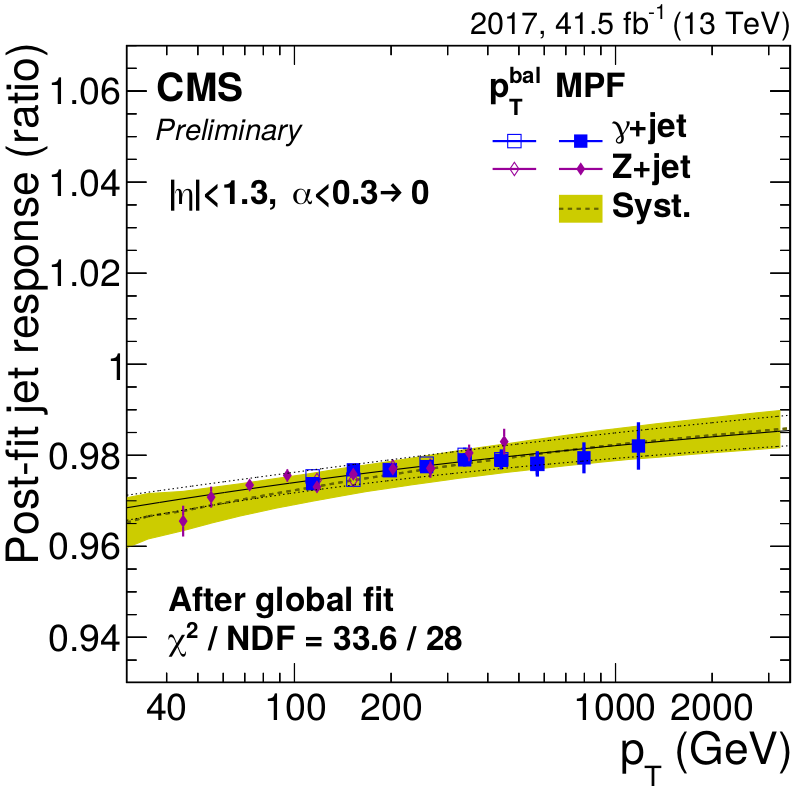
\includegraphics[width=.3\textwidth]{\PhDthesisdir/plots_and_images/from_CMS-DP-2020-019/absolute_pT_residual_2017.png}}
\hfill
\subcaptionbox{Année 2018.\label{subfig-absolute_pT_residual_2018}}[.3\textwidth]
{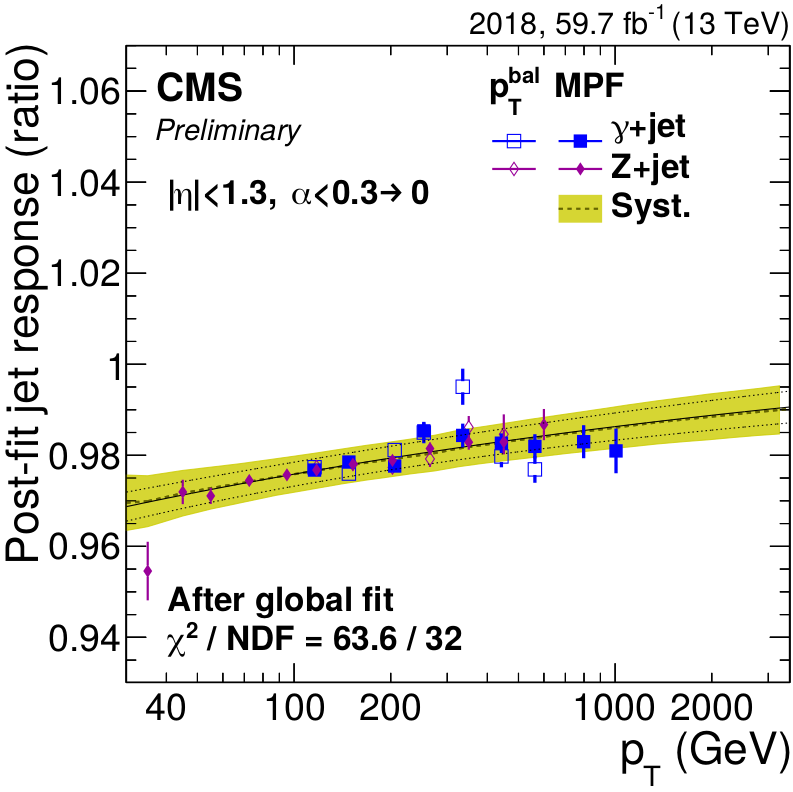
\includegraphics[width=.3\textwidth]{\PhDthesisdir/plots_and_images/from_CMS-DP-2020-019/absolute_pT_residual_2018.png}}
\caption[Correction résiduelle absolue en $\pT$ pour $\abs{\eta}<\num{1.3}$ lors du Run~II.]{Correction résiduelle absolue en $\pT$ pour $\abs{\eta}<\num{1.3}$ lors du Run~II obtenue par ajustement global sur les événements \Gjets, \Zjets\ et multijet~\cite{CMS-DP-2020-019}.}
%Mikko:
%We are now using multijet again, thanks to getting it back to Helsinki, reverting back closer to Run 1 method and actually pushing hard to understand and reduce the systematic uncertainties. And it’s working wonderfully! We’re for sure going to use multijet for all UL samples. Now is the first time it’s actually more constraining at high pT than gamma+jet.
\label{fig-L3ResAbs_RunII}
\end{figure}
\par L'analyse des événements \Gjets\ utilisés dans ces ajustements globaux pour les années 2018, utilisés dans la figure~\ref{subfig-absolute_pT_residual_2018}, et 2017-UL a fait partie de mon travail de thèse.
La phénoménologie de ces événements ainsi que leur analyse sont détaillées dans les sections~\ref{chapter-JERC-section-pheno-GJets} et~\ref{chapter-JERC-section-JES}.
%une fois le ECAL calibré (test de presque chaque cristal en faisceau), calibration du HCAL.
\newpage
\subsubsection{Correction résiduelle de saveur}\label{chapter-JERC-section-CMS-subsec-residuals_flavor}
\begin{wrapfigure}{R}{8cm}
\centering
\vspace{-2\baselineskip}
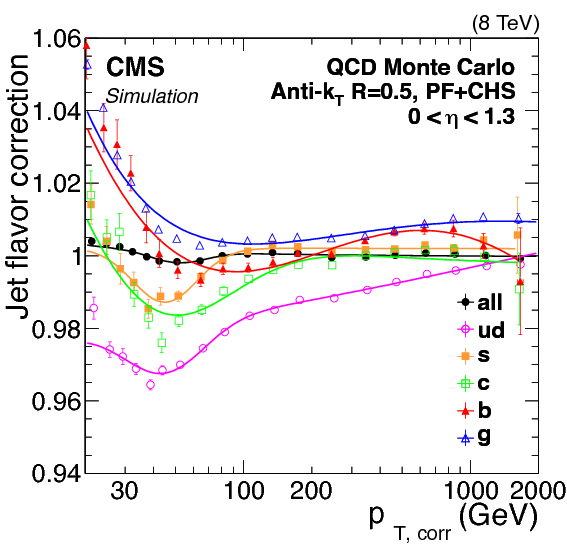
\includegraphics[width=.45\textwidth]{\PhDthesisdir/plots_and_images/from_JERC_RunI/Figure_030-a.png}
\caption[Correction résiduelle de saveur en fonction de l'impulsion du jet.]{Correction résiduelle de saveur en fonction de l'impulsion du jet préalablement corrigée par les corrections décrites dans les sections précédantes, $\pT_\cali$, pour des jets de pseudo-rapidité $\abs{\eta}<\num{1.3}$~\cite{JERC_RunI}.}
\label{fig-chapter-JERC-section-CMS-subsec-PU-JERC_RunI-Figure_030a}
\end{wrapfigure}
Il existe une différence de réponse selon la saveur du jet, majoritairement due à la fragmentation en énergie et la composition du jet qui dépendent de cette saveur~\cite{JERC_RunI}.
Par exemple, les particules de bas \pT\ se retrouvent hors de la zone d'acceptation du détecteur.
Or, des jets initiés par des gluons présentent de nombreuses particules de bas \pT\ par rapport aux jets issus de quarks légers.
Dans une moindre mesure, les jets lourds possèdent également plus de particules de bas \pT\ que les jets de quarks légers suite à la désintégration du hadron lourd\footnote{Le lecteur pourra se référer à la section~\ref{chapter-JERC-section-jets_reco-subsec-flavor} pour plus de détails sur la saveur des jets.}.
La proportion de particules neutres dans le jet est également un des paramètres affectant le plus sa réponse.
\par La correction résiduelle de saveur $\mathcal{C}_\text{Sav}$ à appliquer aux données et aux simulations est obtenue à l'aide de
\PYTHIA~6.4~\cite{pythia6.4}
avec les réglages Z2*~\cite{tunes_2016}
sur des événements dijet, \Zjets\ et \Gjets\ simulés
et est représentée sur la figure~\ref{fig-chapter-JERC-section-CMS-subsec-PU-JERC_RunI-Figure_030a}.
Elle est de moins de \SI{2}{\%} en-deçà de \SI{100}{\GeV} mais peut atteindre \SI{4}{\%} à bas \pT.
\subsection{Incertitude sur la correction en énergie des jets}\label{chapter-JERC-section-CMS-subsec-unc}
Chacune des étapes de la JEC comporte des incertitudes liées aux effets systématiques et, dans une moindre mesure, statistiques.
La maîtrise de ces incertitudes est un enjeu important pour de nombreuses analyses de la collaboration CMS où elles constituent une des sources d'incertitude les plus importantes.
\begin{figure}[p]
\centering
\subcaptionbox{En fonction de $\pT$ pour $\abs{\eta}=0$ en 2016.\label{subfig-Syst_uncs_pT_2016}}[.45\textwidth]
{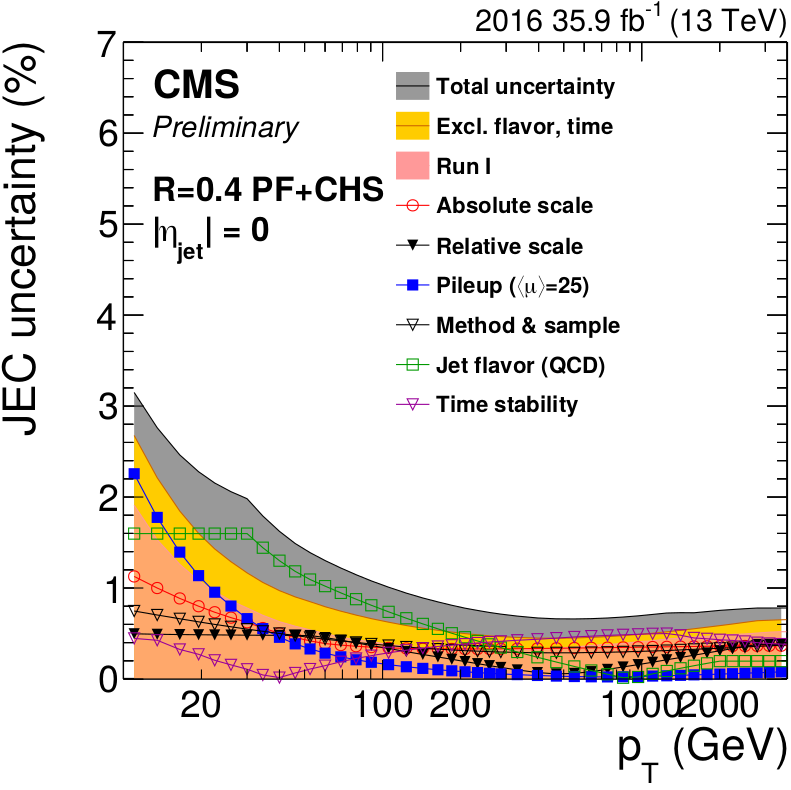
\includegraphics[width=.45\textwidth]{\PhDthesisdir/plots_and_images/from_CMS-DP-2020-019/Syst_uncs_pT_2016.png}\vspace{-.5\baselineskip}}
\hfill
\subcaptionbox{En fonction de $\eta$ pour $\pT=\SI{30}{\GeV}$ en 2016.\label{subfig-Syst_uncs_eta_2016}}[.45\textwidth]
{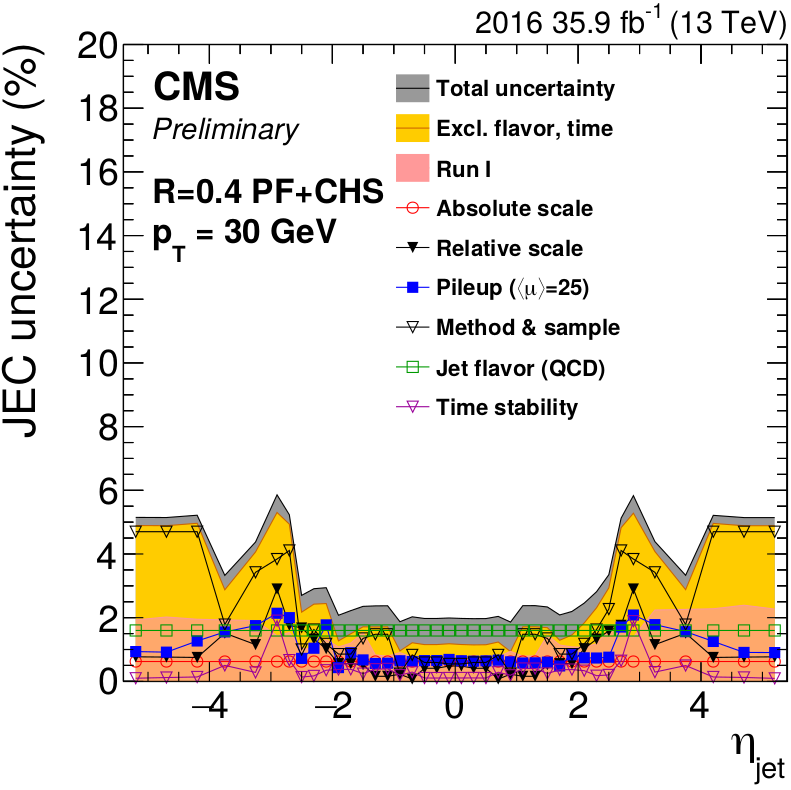
\includegraphics[width=.45\textwidth]{\PhDthesisdir/plots_and_images/from_CMS-DP-2020-019/Syst_uncs_eta_2016.png}\vspace{-.5\baselineskip}}

\vspace{.75\baselineskip}

\subcaptionbox{En fonction de $\pT$ pour $\abs{\eta}=0$ en 2017.\label{subfig-Syst_uncs_pT_2017}}[.45\textwidth]
{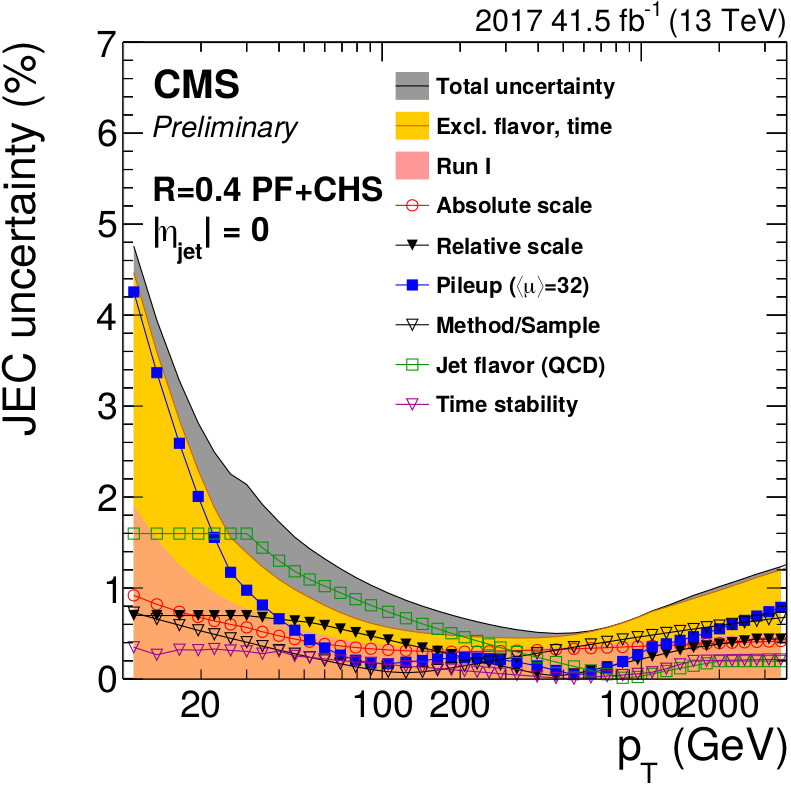
\includegraphics[width=.45\textwidth]{\PhDthesisdir/plots_and_images/from_CMS-DP-2020-019/Syst_uncs_pT_2017.png}\vspace{-.5\baselineskip}}
\hfill
\subcaptionbox{En fonction de $\eta$ pour $\pT=\SI{30}{\GeV}$ en 2017.\label{subfig-Syst_uncs_eta_2017}}[.45\textwidth]
{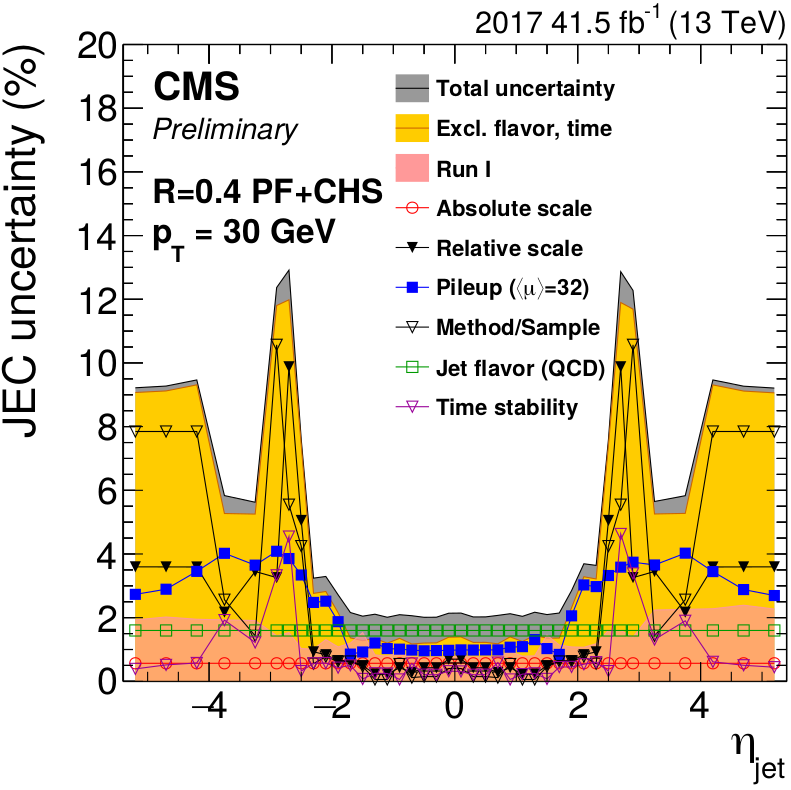
\includegraphics[width=.45\textwidth]{\PhDthesisdir/plots_and_images/from_CMS-DP-2020-019/Syst_uncs_eta_2017.png}\vspace{-.5\baselineskip}}

\vspace{.75\baselineskip}

\subcaptionbox{En fonction de $\pT$ pour $\abs{\eta}=0$ en 2018.\label{subfig-Syst_uncs_pT_2018}}[.45\textwidth]
{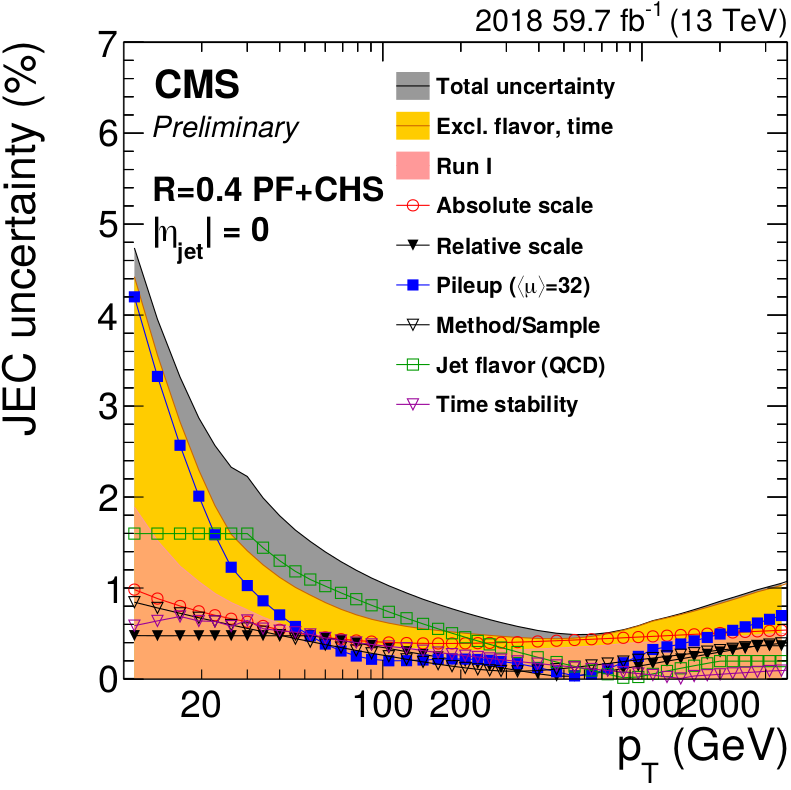
\includegraphics[width=.45\textwidth]{\PhDthesisdir/plots_and_images/from_CMS-DP-2020-019/Syst_uncs_pT_2018.png}\vspace{-.5\baselineskip}}
\hfill
\subcaptionbox{En fonction de $\eta$ pour $\pT=\SI{30}{\GeV}$ en 2018.\label{subfig-Syst_uncs_eta_2018}}[.45\textwidth]
{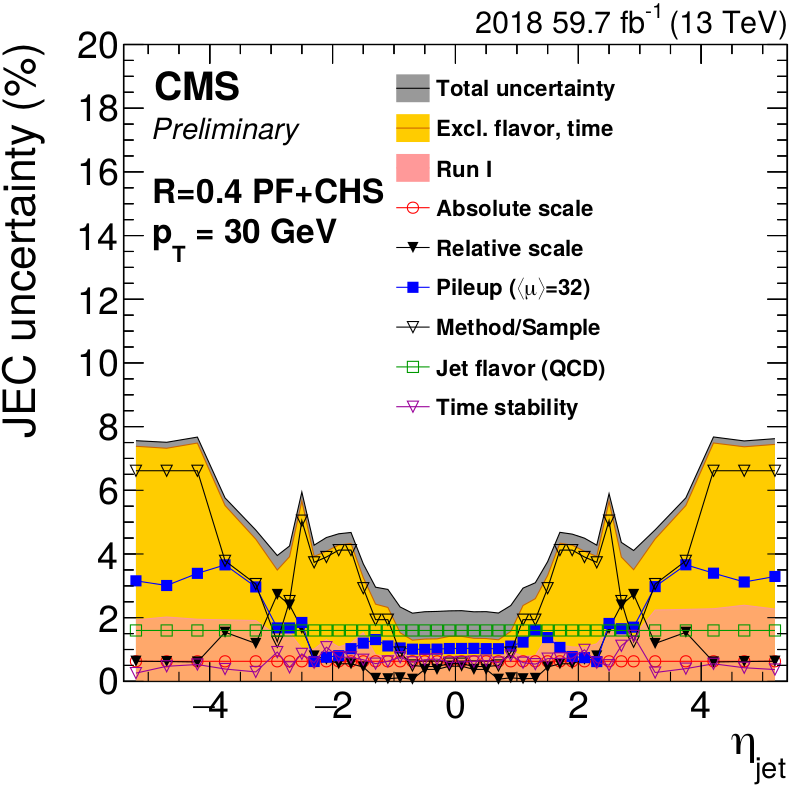
\includegraphics[width=.45\textwidth]{\PhDthesisdir/plots_and_images/from_CMS-DP-2020-019/Syst_uncs_eta_2018.png}\vspace{-.5\baselineskip}}

\caption[Incertitudes relatives sur la JEC en fonction de \pT\ et $\eta$ lors du Run~II.]{Incertitudes relatives sur la JEC lors du Run~II~\cite{CMS-DP-2020-019}.}
\label{fig-Syst_uncs_JEC_RunII}
\end{figure}
Les sources d'incertitude considérées pour la JEC sont réparties en six groupes~\cite{CMS-DP-2020-019}:
\begin{description}
\item[Échelle absolue] ou \emph{Absolute scale} sur les légendes des figures~\ref{subfig-Syst_uncs_pT_2016} à~\ref{subfig-Syst_uncs_eta_2018}.
Cette incertitude prend en compte l'échelle en énergie des objets de référence utilisés pour obtenir la correction résiduelle absolue en \pT\ décrite dans la section~\ref{chapter-JERC-section-CMS-subsec-residuals_pT} ainsi que les effets de l'ISR et du FSR\footnote{L'\emph{Initial State Radiation} et le \emph{Final State Radiation} sont abordés dans la section~\ref{chapter-JERC-section-pheno-GJets}.}.
\item[Échelle relative] ou \emph{Relative scale} sur les légendes des figures~\ref{subfig-Syst_uncs_pT_2016} à~\ref{subfig-Syst_uncs_eta_2018}.
Cette incertitude est principalement due à la JER qui s'applique à l'objet de référence dans la correction résiduelle relative en $\eta$ décrite dans la section~\ref{chapter-JERC-section-CMS-subsec-residuals_eta} ainsi qu'aux effets de l'ISR et du FSR.
\item[Empilement] ou \emph{Pileup} sur les légendes des figures~\ref{subfig-Syst_uncs_pT_2016} à~\ref{subfig-Syst_uncs_eta_2018}.
Il s'agit de rendre compte de l'incertitude sur la détermination de la contribution additionnelle de l'empilement au niveau particule.
Une incertitude de \SI{5}{\%} sur le rapport données sur simulations de cette contribution, obtenue à l'aide de la méthode de cône aléatoire, est considérée.
La différence résiduelle entre la contribution obtenue par cône aléatoire et la contribution réelle extraite des simulations est également prise en compte.
\item[Méthode et jeux de données] ou \emph{Method \& sample} sur les légendes des figures~\ref{subfig-Syst_uncs_pT_2016} à~\ref{subfig-Syst_uncs_eta_2018}.
Cette incertitude correspond aux écarts observés entre les méthodes utilisant les réponses~\Rbal\ et~\RMPF\ d'une part et entre les analyses utilisant les événements \Zjets, \Gjets\ et dijet d'autre part.
\item[Saveur] ou \emph{Jet flavor} sur les légendes des figures~\ref{subfig-Syst_uncs_pT_2016} à~\ref{subfig-Syst_uncs_eta_2018}.
L'incertitude sur la dépendance en saveur de la réponse des jets dans les simulations est estimée à partir de la différence entre deux générateurs,
\PYTHIA~\cite{pythia6.4}
et
\HERWIG~\cite{herwig}.
\item[Stabilité temporelle] ou \emph{Time stability} sur les légendes des figures~\ref{subfig-Syst_uncs_pT_2016} à~\ref{subfig-Syst_uncs_eta_2018}.
La JEC est déterminée pour chaque période de prise de donnée chaque année. Les écarts observés entre ces périodes sont inclus dans cette source d'incertitude.
\end{description}
La figure~\ref{fig-Syst_uncs_JEC_RunII} résume les valeurs de ces incertitudes pour les trois années du Run~II.
L'incertitude globale sur la JEC est généralement inférieure à \SI{2}{\%}, excepté pour les cas $\pT\leq\SI{30}{\GeV}$ ou $\abs{\eta}\geq\num{2}$ où elle peut être de l'ordre de \SI{10}{\%}.
%\subsection{Bilan de la correction en énergie des jets}
%\begin{equation}
%\pT_\cali =
%\underbrace{\underbrace{\underbrace{\pT_\reco^\text{CHS}
%\times
%\mathcal{C}_\text{PU}(\pT_\reco^\text{CHS}, \eta, A_j, \rho)}_{\pT_\reco'}
%\times
%\mathcal{C}_\text{Rép}(\pT_\reco', \eta)}_{\pT_\reco''}
%\times
%\mathcal{C}_\text{Res}(\pT_\reco'', \eta)}_{\pT_\reco'''}
%\times
%\mathcal{C}_\text{Sav}(\pT_\reco''', \eta)
%\end{equation}
\subsection{Correction de la résolution en énergie}\label{chapter-JERC-section-CMS-subsec-JER}
La résolution en énergie des jets, notée JER, est de l'ordre de \SI{10}{\%} pour des jets avec $\pT\geq\SI{50}{\GeV}$ et peut atteindre environ \SI{40}{\%} pour des jets de bas \pT\ et un empilement important~\cite{JERC_RunI}.
Cette résolution est donc bien moins bonne que celles d'autres objets physiques tels que les électrons (\num{2} à \SI{5}{\%}), les muons (\num{1} à \SI{6}{\%}) et les photons (environ \SI{1}{\%}), ce qui peut introduire des biais importants dans les analyses cherchant des résonances étroites, par exemple.
\par La JER est définie comme la largeur de la gaussienne obtenue par un ajustement sur la distribution de $R_\cali$ des jets, \ie\ $\pT_\cali/\pT_\ptcl$.
Sa mesure est réalisée à l'aide d'événements \Gjets\ et \Zjets\ et les résultats obtenus lors du Run~I sont présentés sur la figure~\ref{subfig-chapter-JERC-section-CMS-subsec-JER-JERC_RunI-Figure_036-b}.
Elle est définie comme une fonction de $\pT_\ptcl$, $\eta$ et $\mu$.
\par La JER observée dans les simulations diffère de celle observée dans les données, elle est légèrement meilleure.
Afin de pouvoir réaliser des analyses comparant données et simulations, il est nécessaire d'avoir une JER comparable dans ces deux catégories d'événements.
La JER des simulations est ainsi détériorée par un facteur d'échelle (JER SF), déterminé à partir d'événements \Gjets\ et dijet et défini en fonction de $\eta$.
Les résultats obtenus lors du Run~II sont présentés sur la figure~\ref{subfig-chapter-JERC-section-CMS-subsec-JER-JER_SF_RunII}.
Le principe est le même que pour les corrections résiduelles décrites dans les sections~\ref{chapter-JERC-section-CMS-subsec-residuals_eta} et~\ref{chapter-JERC-section-CMS-subsec-residuals_pT}. Au lieu de s'intéresser à la moyenne de la distribution, c'est sa largeur qui est étudiée.
\begin{figure}[h]
\centering
\subcaptionbox{JER en fonction de \pT\ dans le barillet de CMS ($\abs{\eta}<\num{1.3}$) pour différentes valeurs d'interactions d'empilement $\mu$ lors du Run~I~\cite{JERC_RunI}.\label{subfig-chapter-JERC-section-CMS-subsec-JER-JERC_RunI-Figure_036-b}}[.45\textwidth]
{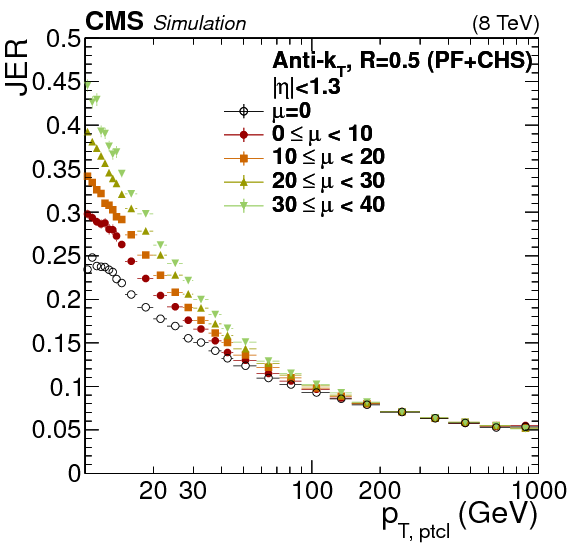
\includegraphics[width=.45\textwidth]{\PhDthesisdir/plots_and_images/from_JERC_RunI/Figure_036-b.png}}
\hfill
\subcaptionbox{Facteurs d'échelle de la résolution en énergie des jets en fonction de $\eta$ lors du Run~II~\cite{CMS-DP-2020-019}.\label{subfig-chapter-JERC-section-CMS-subsec-JER-JER_SF_RunII}}[.45\textwidth]
{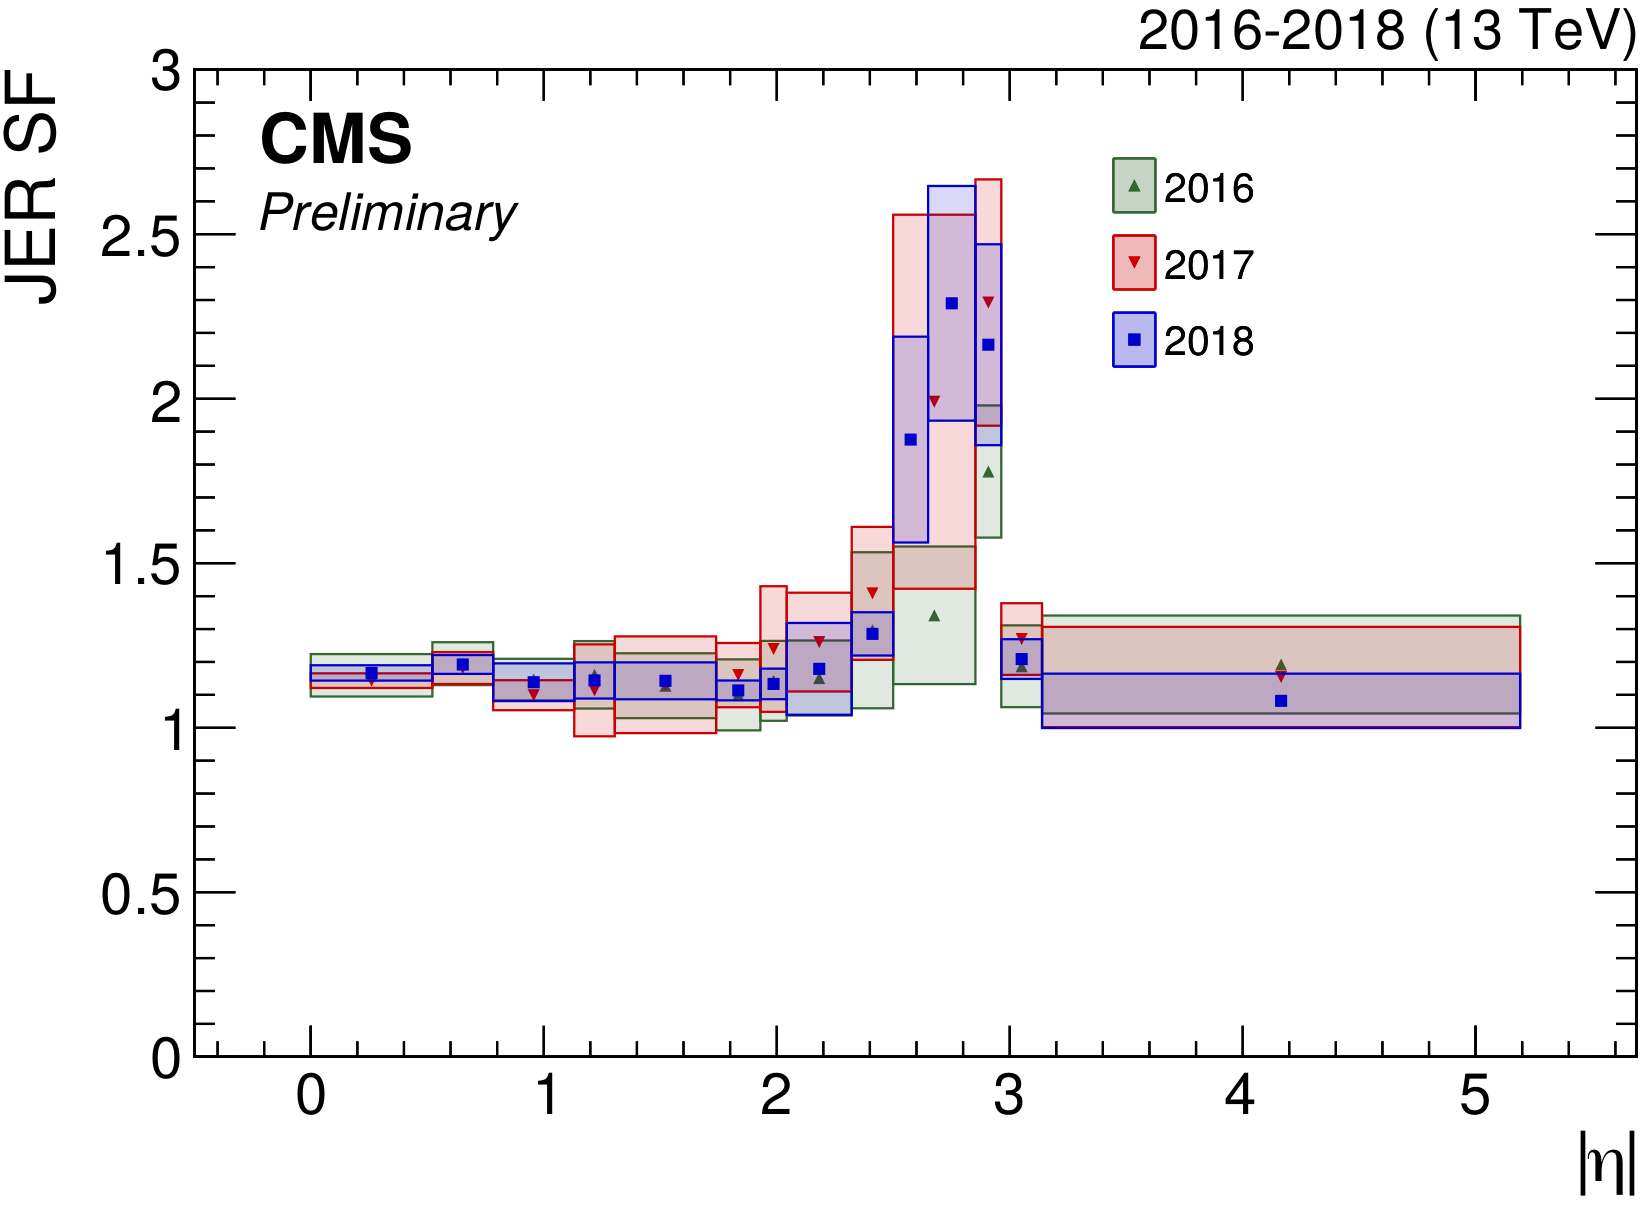
\includegraphics[width=.45\textwidth]{\PhDthesisdir/plots_and_images/from_CMS-DP-2020-019/JER_SF_RunII.png}}
\caption[Résolution en énergie des jets.]{Résolution en énergie des jets dans les simulations et facteurs d'échelle à leur appliquer.}
\label{fig-chapter-JERC-section-CMS-subsec-JER}
\end{figure}
\par L'analyse des événements \Gjets\ utilisés pour les années 2018 et 2017-UL a fait partie de mon travail de thèse.
La phénoménologie de ces événements ainsi que leur analyse sont détaillées dans les sections~\ref{chapter-JERC-section-pheno-GJets} et~\ref{chapter-JERC-section-JER}.


\section{Phénoménologie des événements \Gjets}\label{chapter-JERC-section-pheno-GJets}
Les événements \Gjets\ peuvent être utilisés afin d'obtenir la correction résiduelle absolue en \pT\ des jets, introduite dans la section~\ref{chapter-JERC-section-CMS-subsec-residuals_pT}, ainsi que la résolution en énergie des jets. Les analyses correspondantes sont abordées dans les sections~\ref{chapter-JERC-section-JES} et~\ref{chapter-JERC-section-JER}.
\subsection{Principe des événements \Gjets\ et réponse balancée}
L'état final d'un événement \Gjets\ comporte un jet à calibrer d'une part et un photon utilisé comme objet de référence d'autre part.
Sur la figure~\ref{fig-chapter-JERC-section-pheno-GJets-photon_resolution}, la résolution sur les photons est inférieure à \SI{4}{\%} et de l'ordre du pourcent dans le barillet. Dans le cas des jets, sur la figure~\ref{subfig-chapter-JERC-section-CMS-subsec-JER-JERC_RunI-Figure_036-b}, la résolution minimale est de \SI{5}{\%}.
L'utilisation de photons comme objet de référence est donc justifiée.
\begin{figure}[h]
\centering
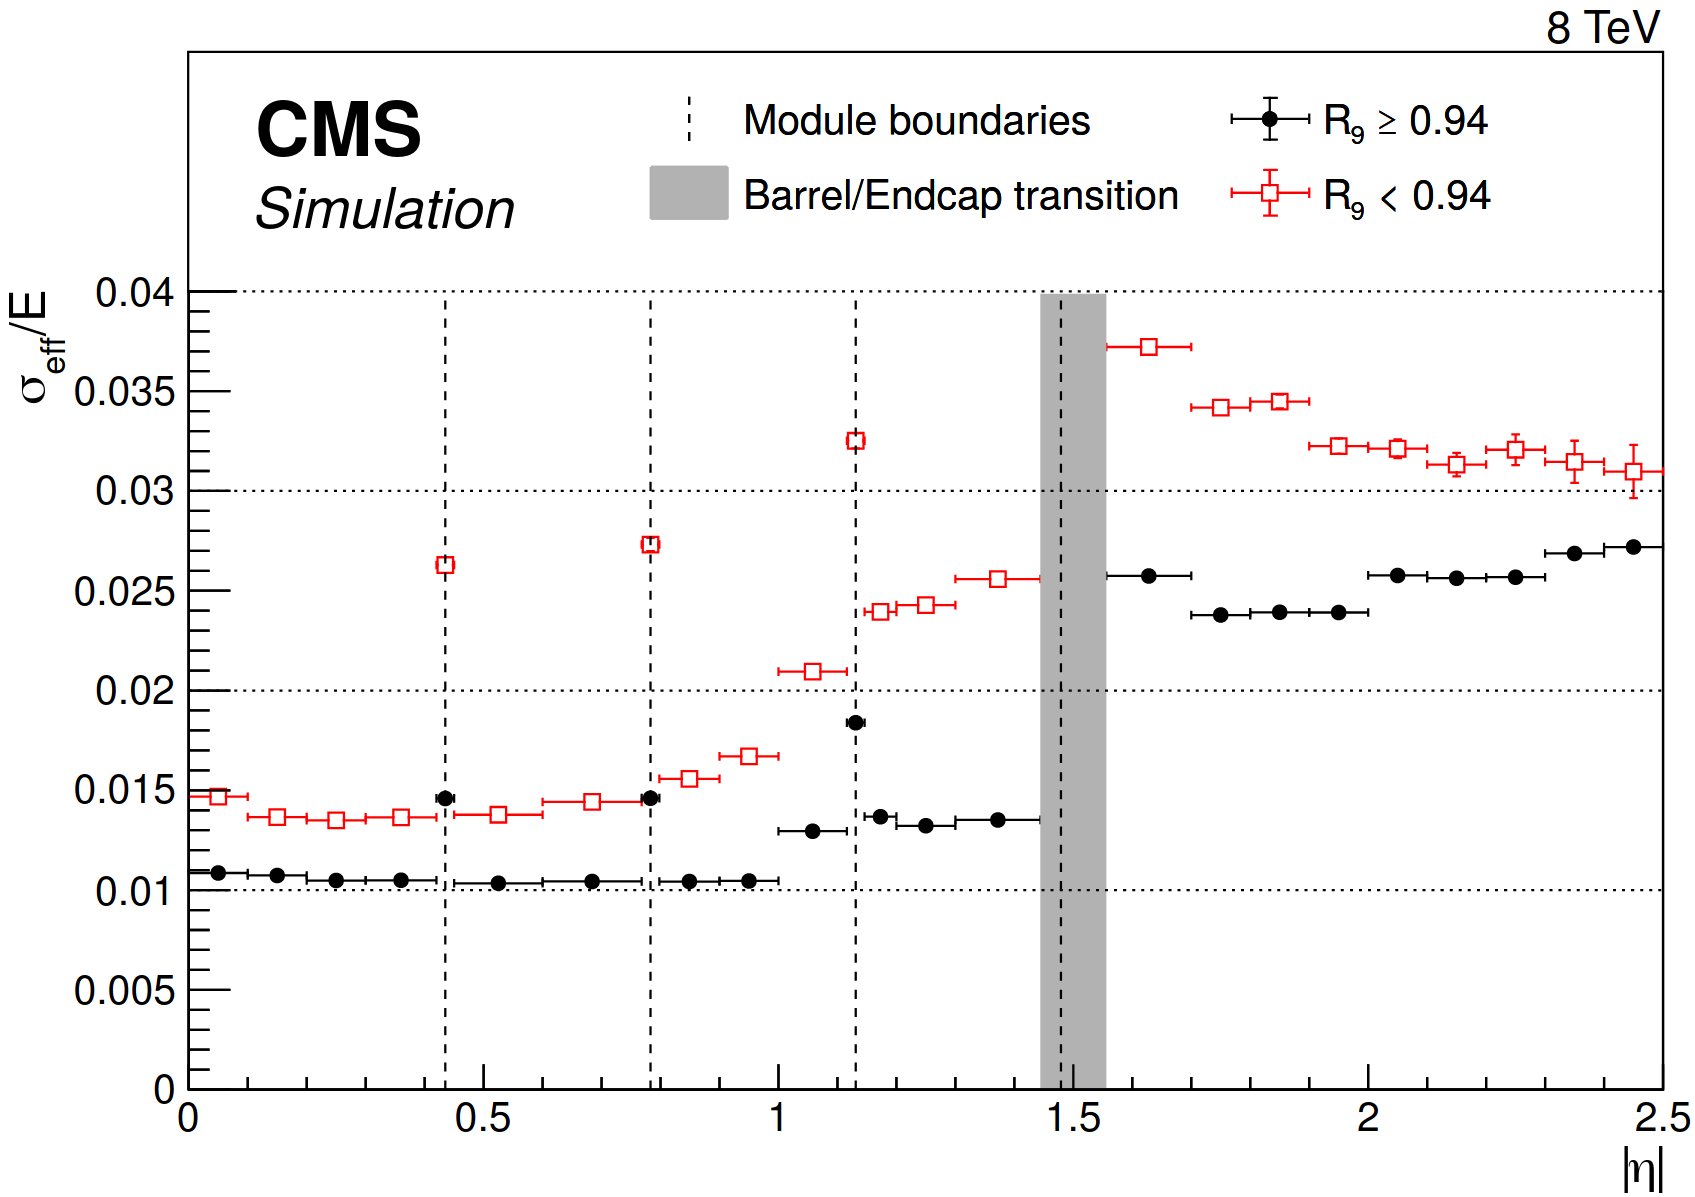
\includegraphics[width=.6\textwidth]{\PhDthesisdir/contents/chapter-JERC/phenomenologie/img_from_photon_ID_2015/photon_resolution.png}
\caption[Résolution en énergie des photons.]{Résolution relative en énergie des photons en fonction de $\eta$ pour des événements simulés $\higgs\to\photon\photon$~\cite{photon_ID_2015}. La variable $R_9$ est définie page~\pageref{eq-R9_definition}.}
\label{fig-chapter-JERC-section-pheno-GJets-photon_resolution}
\end{figure}
\par Des diagrammes de Feynman correspondant à des événements \Gjets\ sont présentés sur la figure~\ref{fig-fgraph-gamma_plus_jets}.
Ces événements ne comportent pas de neutrino issu de l'interaction dure\footnote{Des neutrinos peuvent apparaître lors de la formation du jet.}, il n'y a donc pas d'énergie transverse manquante due à la physique de ces événements.
L'impulsion transverse étant nulle dans l'état initial, par conservation, elle est nulle dans l'état final. Le photon et le jet sont donc balancés, \ie
\begin{equation}
\vpT_\ptcl^{\photon} + \vpT_\ptcl^\text{jet} = \vec{0}
\Rightarrow
\pT_\ptcl^{\photon} = \pT_\ptcl^\text{jet}
\mend
\end{equation}
\begin{figure}[h]
\centering\vspace{\baselineskip}
\subcaptionbox{\label{subfig-fgraph-gq_qGamma_S}}[.3\textwidth]
{\begin{fmffile}{gq_qGamma_S}\fmfstraight
\begin{fmfchar*}(20,20)
  \fmfleft{i1,i2}
  \fmfright{o1,o2}
  \fmf{gluon}{i2,v1}
  \fmf{fermion}{i1,v1,v2,o2}
  \fmf{photon}{v2,o1}
  \fmflabel{\gluon}{i2}
  \fmflabel{\quark}{i1}
  \fmflabel{\quark}{o2}
  \fmflabel{\photon}{o1}
  \fmfdot{v1,v2}
\end{fmfchar*}
\end{fmffile}\vspace{\baselineskip}}
\hfill
\subcaptionbox{\label{subfig-fgraph-gq_qGamma_T}}[.3\textwidth]
{\begin{fmffile}{gq_qGamma_T}\fmfstraight
\begin{fmfchar*}(20,20)
  \fmfleft{i1,i2}
  \fmfright{o1,o2}
  \fmf{gluon}{i2,v2}
  \fmf{fermion}{i1,v1,v2,o2}
  \fmf{photon}{v1,o1}
  \fmflabel{\gluon}{i2}
  \fmflabel{\quark}{i1}
  \fmflabel{\quark}{o2}
  \fmflabel{\photon}{o1}
  \fmfdot{v1,v2}
\end{fmfchar*}
\end{fmffile}\vspace{\baselineskip}}
\hfill
\subcaptionbox{\label{subfig-fgraph-qq_gGamma}}[.3\textwidth]
{\begin{fmffile}{qq_gGamma}\fmfstraight
\begin{fmfchar*}(20,20)
  \fmfleft{i1,i2}
  \fmfright{o1,o2}
  \fmf{gluon}{v2,o2}
  \fmf{fermion}{i1,v1,v2,i2}
  \fmf{photon}{v1,o1}
  \fmflabel{\antiquark}{i2}
  \fmflabel{\quark}{i1}
  \fmflabel{\gluon}{o2}
  \fmflabel{\photon}{o1}
  \fmfdot{v1,v2}
\end{fmfchar*}
\end{fmffile}\vspace{\baselineskip}}
\caption[Diagrammes de Feynman donnant un photon et un jet dans l'état final.]{Exemples de diagrammes de Feynman de processus physiques donnant un photon et un jet dans l'état final.}
\label{fig-fgraph-gamma_plus_jets}
\end{figure}
\par L'impulsion transverse du jet doit donc être égale à celle du photon, objet de référence.
La bonne résolution en énergie sur les photons permet de considérer que leur impulsion transverse au niveau reconstruit est égale à leur impulsion transverse au niveau particule.
Ainsi, la méthode de la balance introduite dans la section~\ref{chapter-JERC-section-CMS-subsec-residuals} permet de définir
\begin{equation}
\Rbal = \frac{\pT_\reco^\text{jet}}{\pT^{\photon}}
\mend[,]
\end{equation}
qui doit valoir 1 après correction.
Cette méthode est performante pour les événements à un photon et un jet dont la topologie est représentée sur la figure~\ref{subfig-Gamma_plus_jet_basic_event}.
\begin{figure}[h]
\centering
\subcaptionbox{Topologie typique des événements correspondant aux diagrammes de la figure~\ref{fig-fgraph-gamma_plus_jets}.\label{subfig-Gamma_plus_jet_basic_event}}[.45\textwidth]
{\includegraphics[width=.45\textwidth,height=.25\textheight,keepaspectratio]{\PhDthesisdir/plots_and_images/Event_displays/JERC/Gamma_plus_jet.tex}}
\hfill
\subcaptionbox{Topologie typique des événements correspondant au diagramme de la figure~\ref{subfig-fgraph-gq_qGamma_S-FSR_2jets}.\label{subfig-Gamma_plus_two_jets}}[.45\textwidth]
{\includegraphics[width=.45\textwidth,height=.25\textheight,keepaspectratio]{\PhDthesisdir/plots_and_images/Event_displays/JERC/Gamma_plus_2jets.tex}}
\caption{Topologies typiques des événements \Gjets.}
\label{fig-Gamma_plus_jet_events}
\end{figure}
\subsection{Activité additionnelle des jets}\label{chapter-JERC-section-pheno-GJets-subsec-effets_radiatifs}
Une activité additionnelle des jets peut survenir et altérer la topologie des événements \Gjets.
Un photon peut être émis dans l'état initial (ISR, \emph{Initial State Radiation}) ou dans l'état final (FSR, \emph{Final State Radiation}), ce qui correspond aux diagrammes de Feynman des figures~\ref{subfig-fgraph-gq_qGamma_S-ISR_2photons} et~\ref{subfig-fgraph-gq_qGamma_S-FSR_2photons}.
Un système composé d'un des photons et du jet n'est donc pas balancé dans ce cas.
Il est possible de supprimer ce biais en imposant la présence d'un seul photon dans l'événement.
La section efficace de production d'événements \Gjets\ à \SI{13}{\TeV} est importante~\cite{Gjet_xsec_2018}, il est donc possible de sélectionner de manière stricte les événements afin d'obtenir une bonne pureté tout en conservant une statistique suffisante.
\begin{figure}[h]
\centering\vspace{\baselineskip}
\subcaptionbox{\label{subfig-fgraph-gq_qGamma_S-ISR_2photons}}[.225\textwidth]
{\begin{fmffile}{gq_qGamma_S-ISR_2photons}\fmfstraight
\begin{fmfchar*}(20,20)
  \fmfleft{i1,i2}
  \fmfright{o0,o1,o2}
  \fmf{gluon}{i2,v1}
  \fmf{phantom}{i1,v1}
  \fmf{phantom, tension=2}{v1,v2}
  \fmf{phantom}{v2,o2}
  \fmf{phantom}{v2,o0}
  \fmflabel{\gluon}{i2}
  \fmflabel{\quark}{i1}
  \fmflabel{\quark}{o2}
  \fmflabel{\photon}{o1}
  \fmfdot{v1,v2}
  \fmffreeze
  \fmf{fermion}{i1,v3,v1,v2,o2}
  \fmffreeze
  \fmf{photon}{v2,o1}
  \fmf{photon}{v3,o0}
  \fmflabel{\photon}{o0}
  \fmfdot{v3}
\end{fmfchar*}
\end{fmffile}\vspace{\baselineskip}}
\hfill
\subcaptionbox{\label{subfig-fgraph-gq_qGamma_S-FSR_2photons}}[.225\textwidth]
{\begin{fmffile}{gq_qGamma_S-FSR_2photons}\fmfstraight
\begin{fmfchar*}(20,20)
  \fmfleft{i1,i2}
  \fmfright{o1,o0,o2}
  \fmf{gluon}{i2,v1}
  \fmf{phantom}{i1,v1,v2,o2}
  \fmf{photon}{v2,o1}
  \fmflabel{\gluon}{i2}
  \fmflabel{\quark}{i1}
  \fmflabel{\quark}{o2}
  \fmflabel{\photon}{o1}
  \fmfdot{v1,v2}
  \fmffreeze
  \fmf{fermion}{i1,v1,v2,v3,o2}
  \fmffreeze
  \fmf{photon}{v3,o0}
  \fmflabel{\photon}{o0}
  \fmfdot{v3}
\end{fmfchar*}
\end{fmffile}\vspace{\baselineskip}}
\hfill
\subcaptionbox{\label{subfig-fgraph-gq_qGamma_S-ISR_2jets}}[.225\textwidth]
{\begin{fmffile}{gq_qGamma_S-ISR_2jets}\fmfstraight
\begin{fmfchar*}(20,20)
  \fmfleft{i1,i2}
  \fmfright{o0,o1,o2}
  \fmf{gluon}{i2,v1}
  \fmf{phantom}{i1,v1}
  \fmf{phantom, tension=2}{v1,v2}
  \fmf{phantom}{v2,o2}
  \fmf{phantom}{v2,o0}
  \fmflabel{\gluon}{i2}
  \fmflabel{\quark}{i1}
  \fmflabel{\quark}{o2}
  \fmflabel{\photon}{o1}
  \fmfdot{v1,v2}
  \fmffreeze
  \fmf{fermion}{i1,v3,v1,v2,o2}
  \fmffreeze
  \fmf{photon}{v2,o1}
  \fmf{gluon}{v3,o0}
  \fmflabel{\gluon}{o0}
  \fmfdot{v3}
\end{fmfchar*}
\end{fmffile}\vspace{\baselineskip}}
\hfill
\subcaptionbox{\label{subfig-fgraph-gq_qGamma_S-FSR_2jets}}[.225\textwidth]
{\begin{fmffile}{gq_qGamma_S-FSR_2jets}\fmfstraight
\begin{fmfchar*}(20,20)
  \fmfleft{i1,i2}
  \fmfright{o1,o0,o2}
  \fmf{gluon}{i2,v1}
  \fmf{phantom}{i1,v1}
  \fmf{phantom, tension=2}{v1,v2}
  \fmf{phantom}{v2,o2}
  \fmf{photon}{v2,o1}
  \fmflabel{\gluon}{i2}
  \fmflabel{\quark}{i1}
  \fmflabel{\quark}{o2}
  \fmflabel{\photon}{o1}
  \fmfdot{v1,v2}
  \fmffreeze
  \fmf{fermion}{i1,v1,v2,v3,o2}
  \fmffreeze
  \fmf{gluon}{v3,o0}
  \fmflabel{\gluon}{o0}
  \fmfdot{v3}
\end{fmfchar*}
\end{fmffile}\vspace{\baselineskip}}
\caption[Diagrammes de Feynman de processus avec ISR ou FSR.]{Exemples de diagrammes de Feynman de processus correspondant à des événements avec deux photons (\ref{subfig-fgraph-gq_qGamma_S-ISR_2photons}, \ref{subfig-fgraph-gq_qGamma_S-FSR_2photons}) ou deux jets (\ref{subfig-fgraph-gq_qGamma_S-ISR_2jets}, \ref{subfig-fgraph-gq_qGamma_S-FSR_2jets}) dans l'état final, dus à l'ISR (\ref{subfig-fgraph-gq_qGamma_S-ISR_2photons}, \ref{subfig-fgraph-gq_qGamma_S-ISR_2jets}) ou au FSR (\ref{subfig-fgraph-gq_qGamma_S-FSR_2photons}, \ref{subfig-fgraph-gq_qGamma_S-FSR_2jets}).}
\label{fig-fgraph-gamma_plus_jets-ISR-FSR}
\end{figure}
\par L'ISR et le FSR peuvent aussi produire un gluon, ce qui correspond aux diagrammes de Feynman des figures~\ref{subfig-fgraph-gq_qGamma_S-ISR_2jets} et~\ref{subfig-fgraph-gq_qGamma_S-FSR_2jets}.
Plusieurs jets sont alors présents dans l'état final et sont ordonnés par impulsion transverse décroissante.
La topologie d'un tel événement est illustrée sur la figure~\ref{subfig-Gamma_plus_two_jets}.
Il est possible de réduire le nombre d'événements avec ISR ou FSR en imposant une condition sur les directions du photon et du premier jet qui doivent être opposées.
Toutefois, la plupart des événements présentent plusieurs jets dans la direction opposée au photon.
La réponse balancée est alors considérée entre le photon et le premier jet, \ie\ le jet d'impulsion transverse la plus grande. Ainsi,
\begin{equation}
\Rbal = \frac{\pT_\reco^\text{jet 1}}{\pT^{\photon}}
\mend
\end{equation}
\par En complément de la réponse balancée, la réponse MPF, définie comme
\begin{equation}
\RMPF = 1 + \frac{\vpT^{\photon}\cdot\vMET}{\abs{\vpT^{\photon}}^2}
\mend[,]
\end{equation}
est également analysée.
Les impulsions de toutes les particules présentes étant considérées, \RMPF\ est moins sensible à l'activité additionnelle que \Rbal.
L'utilisation conjointe de \RMPF\ avec \Rbal\ permet d'obtenir des résultats complémentaires.
Des écarts significatifs observés entre les deux méthodes indiqueraient ainsi des effets incompris, nécessitant de plus amples investigations.


\section{Correction résiduelle absolue en \pT\ avec les événements \Gjets}\label{chapter-JERC-section-JES}
Durant ma thèse, j'étais responsable de la mesure de cette correction avec les événements \Gjets\ pour les années 2018 et 2017-UL pour la collaboration CMS.
Cette section présente la sélection des événements \Gjets, leur analyse et les derniers résultats obtenus pour l'année 2018.
\subsection{Événements utilisés}\label{chapter-JERC-section-JES-subsec-evt_select}
\subsubsection{Ensembles d'événements analysés}
%18 data
%     Run2018A-17Sep2018-v2
%     /EGamma/Run2018A-17Sep2018-v2/MINIAOD
%     13654.355526985
%     
%     Run2018B-17Sep2018-v1
%     /EGamma/Run2018B-17Sep2018-v1/MINIAOD
%     7057.825158567
%     
%     Run2018C-17Sep2018-v1
%     /EGamma/Run2018C-17Sep2018-v1/MINIAOD
%     6894.770971269
%     
%     Run2018D-PromptReco-v2
%     /EGamma/Run2018D-PromptReco-v2/MINIAOD
%     31066.589629726
%
%18 MC
%     GJet_Pt-15To6000_RunIIAutumn18MiniAOD-102X
%     /GJet_Pt-15To6000_TuneCP5-Flat_13TeV_pythia8/RunIIAutumn18MiniAOD-102X_upgrade2018_realistic_v15-v1/MINIAODSIM
%     283000.0
%
%17UL data
%     Run2017B-09Aug2019_UL2017-v1
%     /SinglePhoton/Run2017B-09Aug2019_UL2017-v1/MINIAOD
%     4793.961426839
%     
%     Run2017C-09Aug2019_UL2017-v1
%     /SinglePhoton/Run2017C-09Aug2019_UL2017-v1/MINIAOD
%     9631.214820913
%     
%     Run2017D-09Aug2019_UL2017-v1
%     /SinglePhoton/Run2017D-09Aug2019_UL2017-v1/MINIAOD
%     4247.682053046
%     
%     Run2017E-09Aug2019_UL2017-v1
%     /SinglePhoton/Run2017E-09Aug2019_UL2017-v1/MINIAOD
%     9313.642401775
%     
%     Run2017F-09Aug2019_UL2017-v1
%     /SinglePhoton/Run2017F-09Aug2019_UL2017-v1/MINIAOD
%     13539.378417564
%
%
%17UL MC
%     GJets_HT-40To100_RunIISummer19MiniAOD-106X
%     /GJets_HT-40To100_TuneCP5_13TeV-madgraphMLM-pythia8/RunIISummer19UL17MiniAOD-106X_mc2017_realistic_v6-v1/MINIAODSIM
%     18700.0
%     
%     GJets_HT-100To200_RunIISummer19MiniAOD-106X
%     /GJets_HT-100To200_TuneCP5_13TeV-madgraphMLM-pythia8/RunIISummer19UL17MiniAOD-4cores5k_106X_mc2017_realistic_v6-v1/MINIAODSIM
%     8640.0
%     
%     GJets_HT-200To400_RunIISummer19MiniAOD-106X
%     /GJets_HT-200To400_TuneCP5_13TeV-madgraphMLM-pythia8/RunIISummer19UL17MiniAOD-106X_mc2017_realistic_v6-v1/MINIAODSIM
%     2185.0
%     
%     GJets_HT-400To600_RunIISummer19MiniAOD-106X
%     /GJets_HT-400To600_TuneCP5_13TeV-madgraphMLM-pythia8/RunIISummer19UL17MiniAOD-106X_mc2017_realistic_v6-v1/MINIAODSIM
%     259.9
%     
%     GJets_HT-600ToInf_RunIISummer19MiniAOD-106X
%     /GJets_HT-600ToInf_TuneCP5_13TeV-madgraphMLM-pythia8/RunIISummer19UL17MiniAOD-106X_mc2017_realistic_v6-v1/MINIAODSIM
%     85.31 \pm 0.2564
\paragraph{Données}
Les jeux de données utilisés pour 2018 et 2017-UL sont basés sur la présence d'un photon dans l'état final.
Pour chacune de ces années, plusieurs périodes (\emph{runs}) sont considérées, celles des collisions \proton\proton, dont la liste et les luminosités correspondantes sont présentées dans le tableau~\ref{tab-Runs_and_lumis_2018_and_2017UL_GJet}.
\begin{table}[h]
\centering
\begin{tabular}{ccc}
\toprule
\multirow{2}{*}{Run} & \multicolumn{2}{c}{Luminosité (\SI{}{\femto\barn^{-1}})} \\
\cmidrule(lr){2-3}
 & 2018 & 2017-UL \\
\midrule
A & \num{13.98} & - \\
B & \num{7.06} & \num{4.823} \\
C & \num{6.90} & \num{9.664} \\
D & \num{31.75} & \num{4.252} \\
E & - & \num{9.278} \\
F & - & \num{13.54} \\
\midrule
Total & \num{59.69} & \num{41.57} \\
\bottomrule
\end{tabular}
\caption{Liste des périodes de prise de données considérées et luminosités correspondantes.}
\label{tab-Runs_and_lumis_2018_and_2017UL_GJet}
\end{table}
\paragraph{Simulations}
Les simulations utilisées contiennent des événements \Gjets\ de type $\quark\gluon\to\quark\photon$, comme ceux des figures~\ref{subfig-fgraph-gq_qGamma_S} et~\ref{subfig-fgraph-gq_qGamma_T}, et $\quark\quark\to\gluon\photon$, comme celui de la figure~\ref{subfig-fgraph-qq_gGamma}.
Pour l'année 2018, les événements sont générés en un seul jeu de données
à l'aide de \PYTHIA~8~\cite{pythia8.2}
avec les réglages CP5-Flat~\cite{tunes_2019}
et une énergie dans le centre de masse de \SI{13}{\TeV}.
Dans l'état final, un photon d'impulsion transverse comprise entre \num{15} et \SI{6000}{\GeV} est généré.
Pour l'année 2017-UL, les événements sont générés conjointement
à l'aide de \PYTHIA~8~\cite{pythia8.2}
avec les réglages CP5~\cite{tunes_2019}
et
\MADGRAPHc~\cite{madgraph5}
et une énergie dans le centre de masse de \SI{13}{\TeV}.
Dans l'état final, la somme scalaire des impulsions transverses des jets, notée HT, appartient à un intervalle, définissant ainsi cinq jeux de données.
Les sections efficaces des événements simulés ainsi obtenus sont présentées dans le tableau~\ref{tab-MC_xsec_2018_and_2017UL_GJet}.
\begin{table}[h]
\centering
\begin{tabular}{clc}
\toprule
Année & Caractéristique & Section efficace (\SI{}{\pico\barn})\\
\midrule
2018 & $\pT^{\photon}\in [\num{15}, \num{6000}]\usp\SI{}{\GeV}$ & \num{283000.0}\\
2017-UL & $\text{HT} \in [\num{40}, \num{100}]\usp\SI{}{\GeV}$ & \num{18700.0} \\
2017-UL & $\text{HT} \in [\num{100}, \num{200}]\usp\SI{}{\GeV}$ & \num{8640.0} \\
2017-UL & $\text{HT} \in [\num{200}, \num{400}]\usp\SI{}{\GeV}$ & \num{2185.0} \\
2017-UL & $\text{HT} \in [\num{400}, \num{600}]\usp\SI{}{\GeV}$ & \num{259.9} \\
2017-UL & $\text{HT} > \SI{600}{\GeV}$ & \num{85.31} \\
\bottomrule
\end{tabular}
\caption{Sections efficaces des différents événements \Gjets\ simulés.}
\label{tab-MC_xsec_2018_and_2017UL_GJet}
\end{table}
\subsubsection{Sélection des événements}
Une sélection des événements à considérer est réalisée lors de l'analyse.
En effet, les événements souhaités sont ceux contenant un photon avec un ou plusieurs jets;
un des bruits de fond principal provient d'événements multijet où un des jets est identifié à tort comme un photon.
Cette situation peut arriver lorsqu'une fraction importante de l'énergie de ce jet est portée par un ou plusieurs pions neutres, les \pionnull.
Les \pionnull\ se propagent sur des distances moyennes de \SI{26}{\nano\meter} puis se désintègrent dans \SI{99}{\%} des cas en deux photons~\cite{PDG_booklet_2020}.
Ces particules ne laissent donc aucune trace dans le trajectographe et un dépôt d'énergie dans le ECAL, tout comme les photons issus de l'interaction initiale.
Un tel jet comporte ainsi une signature similaire à un photon d'un événement \Gjet\ autour duquel une activité hadronique existe.
%Les topologies de ces deux types d'événements, semblables, sont représentées sur la figure~\ref{fig-Gamma_plus_jet_events_real_faked}.
%\begin{figure}[h]
%\centering
%\subcaptionbox{Topologie d'un événement dijet, dont un jet contient de nombreux \pionnull.\label{subfig-Gamma_plus_jet_basic_event_dijet_faked}}[.45\textwidth]
%{\includegraphics[width=.45\textwidth,height=.25\textheight,keepaspectratio]{\PhDthesisdir/plots_and_images/Event_displays/JERC/Dijets_pi0s.tex}}
%\hfill
%\subcaptionbox{Topologie d'un vrai événement \Gjet\ avec un peu d'activité hadronique autour du photon.\label{subfig-Gamma_plus_jet_basic_event_real}}[.45\textwidth]{\includegraphics[width=.45\textwidth,height=.25\textheight,keepaspectratio]{\PhDthesisdir/plots_and_images/Event_displays/JERC/Gamma_plus_jet_hadronic_noise.tex}}
%\caption{Topologies d'événements \Gjet\ et dijet.}
%\label{fig-Gamma_plus_jet_events_real_faked}
%\end{figure}
\paragraph{Sélection sur les photons}
Une sélection des photons est appliquée afin de réduire le bruit de fond.
La collaboration CMS propose des critères d'identification des photons (lâche, moyen et strict) s'appuyant sur diverses propriétés du \og candidat \fg{} photon:
\begin{itemize}
\item $H/E$ est le rapport de l'énergie hadronique sur l'énergie électromagnétique associées au photon.
Un photon est sensé déposer son énergie dans le ECAL et ne laisser aucun signal dans le HCAL.
Une faible valeur de $H/E$ est donc compatible avec un photon.
\item $\sigma_{i\eta i\eta}$ est l'étalement en $\eta$ du dépôt d'énergie dans le ECAL.
Cette observable est reliée à la forme de la gerbe électromagnétique.
Un seuil maximal sur $\sigma_{i\eta i\eta}$ est imposé pour l'identification des photons.
\item $I_{CH}$ est l'isolation vis-à-vis des hadrons chargés.
Elle se définit comme le ratio entre la somme des impulsions transverses de tous les hadrons chargés situés à une distance $\Delta R$ du candidat photon dans le plan $(\eta,\phi)$ inférieure à \num{0.3} et l'impulsion transverse du candidat photon lui-même.
\item $I_{NH}$ est l'isolation vis-à-vis des hadrons neutres, analogue à $I_{CH}$.
\item $I_{\photon}$ est l'isolation vis-à-vis des photons autres que le candidat lui-même, analogue à $I_{CH}$.
\end{itemize}
À cet ensemble de variables dont une valeur maximale est admise pour l'identification des photons s'ajoute $R_9$, définie comme
\begin{equation}
R_9 = \frac{E_{3\times3}}{E_{SC}}
\label{eq-R9_definition}
\end{equation}
avec
$E_{3\times3}$ la somme des énergies dans les cristaux du ECAL formant un carré de trois cristaux de côté centré sur le cristal contenant le plus d'énergie dans le \emph{supercluster}, défini dans la section~\ifref{chapter-LHC-section-evt_reco-subsec-ptc_ID}{\ref{chapter-LHC-section-evt_reco-subsec-ptc_ID}}{4.2} du chapitre~\ifref{chapter-LHC}{\ref{chapter-LHC}}{3}.
et
$E_{SC}$
l'énergie dans le \emph{supercluster}~\cite{photon_ID_2015}.
Dans l'analyse des événements \Gjets, il est demandé que $R_9 > \num{0.90}$.
\par Les variables d'isolation sont corrigées afin de prendre en compte l'empilement.
L'isolation corrigée $I^\text{corr}$ s'exprime ainsi en fonction de l'isolation $I$ comme
\begin{equation}
I^\text{corr} = \max\left( I - \rho \times \mathcal{E_A} , 0\right)
\end{equation}
où $\mathcal{E_A}$ est l'aire effective, \ie\ la fraction de l'espace $(\eta,\phi)$ correspondant à la zone d'isolation à corriger pour l'empilement. Les valeurs des aires effectives utilisées sont présentées dans le tableau~\ref{tab-CutBasedPhotonIdentificationRun2-effective_areas}.
\begin{table}[h]
\centering
\begin{tabular}{cccc}
\toprule
Région & Hadrons chargés & Hadrons neutres & Photons \\
\midrule
$\abs{\eta} \leq \num{1.0}$ & \num{0.0112} & \num{0.0668} & \num{0.1113} \\
$\num{1.0} < \abs{\eta} \leq \num{1.479}$ & \num{0.0108} & \num{0.1054} & \num{0.0953} \\
$\num{1.479} < \abs{\eta} \leq \num{2.0}$ & \num{0.0106} & \num{0.0786} & \num{0.0619} \\
$\num{2.0} < \abs{\eta} \leq \num{2.2}$ & \num{0.01002} & \num{0.0233} & \num{0.0837} \\
$\num{2.2} < \abs{\eta} \leq \num{2.3}$ & \num{0.0098} & \num{0.0078} & \num{0.1070} \\
$\num{2.3} < \abs{\eta} \leq \num{2.4}$ & \num{0.0089} & \num{0.0028} & \num{0.1212} \\
$\abs{\eta} > \num{2.4}$ & \num{0.0087} & \num{0.0137} & \num{0.1466} \\
\bottomrule
\end{tabular}
\caption[Aires effectives de correction de l'isolation du photon.]{Valeurs de l'aire effective $\mathcal{E_A}$ utilisée pour corriger la contribution de l'empilement aux isolations des photons vis-à-vis des autres particules.}
\label{tab-CutBasedPhotonIdentificationRun2-effective_areas}
\end{table}
\par De plus, un veto est appliqué aux photons pouvant être reliés à une trace dans le trajectographe.
Ce veto permet de limiter la contamination des photons considérés dans l'analyse par des électrons reconstruits à tort comme des photons.
Les coupures correspondant aux différents critères d'identification des photons ainsi que leurs efficacités d'identification et de réjection sont résumées dans le tableau~\ref{tab-CutBasedPhotonIdentificationRun2}.
\begin{table}[h]
\centering\small
\begin{tabularx}{\textwidth}{Xcccccc}
\toprule
Critère & \multicolumn{2}{c}{Lâche} & \multicolumn{2}{c}{Moyen} & \multicolumn{2}{c}{Strict} \\
\cmidrule(lr){2-3}\cmidrule(lr){4-5}\cmidrule(lr){6-7}
Région & Barillet & Bouchon & Barillet & Bouchon & Barillet & Bouchon\\
\midrule
Efficacité & \SI{90.08}{\%} & \SI{90.65}{\%} & \SI{80.29}{\%} & \SI{80.08}{\%} & \SI{70.24}{\%} & \SI{70.13}{\%} \\
Réjection & \SI{86.25}{\%} & \SI{76.72}{\%} & \SI{89.36}{\%} & \SI{81.85}{\%} & \SI{90.97}{\%} & \SI{84.55}{\%} \\
\midrule
$H/E$ & \num{0.04596} & \num{0.0590} & \num{0.02197} & \num{0.0326} & \num{0.02148} & \num{0.0321} \\
$\sigma_{i\eta i\eta}$ & \num{0.0106} & \num{0.0272} & \num{0.01015} & \num{0.0272} & \num{0.00996} & \num{0.0271} \\
$I_{CH}^\text{corr}$ & \num{1.694} & \num{2.089} & \num{1.141} & \num{1.051} & \num{0.65} & \num{0.517} \\
\multirow{3}{*}{$I_{NH}^\text{corr} \!\!\!\hphantom{I_{\photon}^\text{corr}} \left\lbrace \begin{matrix} \vphantom{0} \\ \vphantom{0} \\ \vphantom{0} \end{matrix} \right. $} & $\num{24.032}$& $\num{19.722}$& $\num{1.189}$& $\num{2.718}$& $\num{0.317}$& $\num{2.716}$\\
& $+ \num{0.01512} \, \pT$& $+ \num{0.011} \, \pT$& $+ \num{0.01512} \, \pT$& $+ \num{0.0117} \, \pT$& $+ \num{0.01512} \, \pT$& $+ \num{0.0117} \, \pT$ \\
& $+ \num{2.259} \pT^{\!2} \! / 10^5$ & $+ \num{2.3} \pT^{\!2} \! / 10^5$ & $+ \num{2.259} \pT^{\!2} \! / 10^5$ & $+ \num{2.3} \pT^{\!2} \! / 10^5$ & $+ \num{2.259} \pT^{\!2} \! / 10^5$ & $+ \num{2.3} \pT^{\!2} \! / 10^5$ \\
\multirow{2}{*}{$I_{\photon}^\text{corr} \!\!\!\hphantom{I_{NH}^\text{corr}} \left\lbrace \begin{matrix} \vphantom{0} \\ \vphantom{0} \end{matrix} \right. $} & $\num{2.876}$ & $\num{4.162}$ & $\num{2.08}$ & $\num{3.867}$ & $\num{2.044}$ & $\num{3.032}$ \\
& $+ \num{0.004017} \, \pT$ & $+ \num{0.0037} \, \pT$ & $+ \num{0.004017} \, \pT$ & $+ \num{0.0037} \, \pT$ & $+ \num{0.004017} \, \pT$ & $+ \num{0.0037} \, \pT$ \\
\bottomrule
\end{tabularx}
\caption[Coupures utilisées pour l'identification des photons.]{Valeurs maximales des observables considérées pour l'identification des photons selon le critère utilisé et la région du détecteur dans laquelle se trouve le candidat photon (barillet pour $\abs{\eta} < \num{1.479}$, bouchon sinon).}
\label{tab-CutBasedPhotonIdentificationRun2}
\end{table}
\par Le critère d'identification des photons retenu dans l'analyse est le critère strict.
Seuls les photons situés dans le barillet sont utilisés car ils présentent la meilleure résolution.
%La figure~\ref{fig-chapter-JERC-section-pheno-GJets-photon_resolution}, page~\pageref{fig-chapter-JERC-section-pheno-GJets-photon_resolution}, montre en effet que ces photons possèdent une résolution relative en énergie de l'ordre de \SI{1}{\%}, contre environ \SI{2.5}{\%} pour les photons des bouchons.
Une coupure sur leur pseudo-rapidité est donc appliquée telle que $\abs{\eta} < \num{1.3}$, excluant également les bords du barillet proches des bouchons.
\par Une étude interne a montré que l'utilisation des photons des bouchons ($\abs{\eta} > \num{1.479}$) permettrait de rajouter près de \SI{30}{\%} d'événements dans les données et de réduire ainsi les incertitudes statistiques.
Les corrections résiduelles obtenues pourraient alors être plus précises.
Toutefois, la résolution en énergie des photons, représentée en fonction de $\abs{\eta}$ sur la figure~\ref{fig-chapter-JERC-section-pheno-GJets-photon_resolution} en page~\pageref{fig-chapter-JERC-section-pheno-GJets-photon_resolution}, est de l'ordre de \SI{1}{\%} dans le barillet contre \SI{2.5}{\%} dans les bouchons.
Cette différence sur la résolution en énergie de l'objet de référence rend délicate la combinaison des photons du barillet et des bouchons dans cette analyse.
Des travaux sont actuellement menés dans cette direction.
\paragraph{Sélection sur les jets}
Les événements présentant un unique photon sélectionné d'après les critères précédents sont retenus.
Avec ce photon doit être présent au moins un jet reconstruit à l'aide de l'algorithme anti-\kT~\cite{Cacciari_antikT} avec un paramètre $R=\num{0.4}$ et respectant les critères définis dans le tableau~\ref{tab-chapter-JERC-section-jets_reco-subsec-jetID-2018} pour les données de 2018 et ceux du tableau~\ref{tab-chapter-JERC-section-jets_reco-subsec-jetID-2017UL} pour les données de 2017-UL.
Ces critères permettent de rejeter les jets issus du bruit de fond avec une efficacité de \SI{99}{\%}.
\par Les jets ainsi sélectionnés sont calibrés en énergie en suivant la procédure décrite dans la section~\ref{chapter-JERC-section-CMS} jusqu'à la correction résiduelle relative en $\eta$ incluse. Ils sont alors triés par impulsion transverse décroissante.
Pour s'assurer d'une bonne balance dans le plan transverse entre le photon et le premier jet, \ie\ celui d'impulsion transverse la plus grande, seuls les événements proposant un écart angulaire $\Delta\phi$ entre le photon et ce jet supérieur à \SI{2.8}{\rad} sont considérés dans la suite.
Le photon et le jet sont donc dos à dos dans le plan transverse.
Il est de plus requis que ce jet soit d'impulsion transverse supérieure à \SI{15}{\GeV}.
\par Si un second jet d'impulsion transverse supérieure à \SI{10}{\GeV} et à \SI{30}{\%} de $\pT^{\photon}$ est présent, l'événement est rejeté.
L'événement est également rejeté si un lepton (électron ou muon) isolé, en pratique hors des jets, est présent.
\par Il a été observé que des régions des calorimètres produisent des signaux menant à des reconstructions biaisées de jets.
De plus, un système de lecture expérimental \og SiPM \fg{} a été installé dans le bouchon du HCAL~\cite{SiPM_CMS_conf}.
Il en résulte des calibrations qui ne sont pas optimales dans les régions correspondantes du détecteur.
Afin d'éviter ces effets, tout événement est rejeté s'il comporte, dans ces régions des calorimètres, un jet utilisé dans l'analyse.
Ces régions sont résumées sur la figure~\ref{fig-hotjets2017UL}.
\begin{figure}[h]
\centering
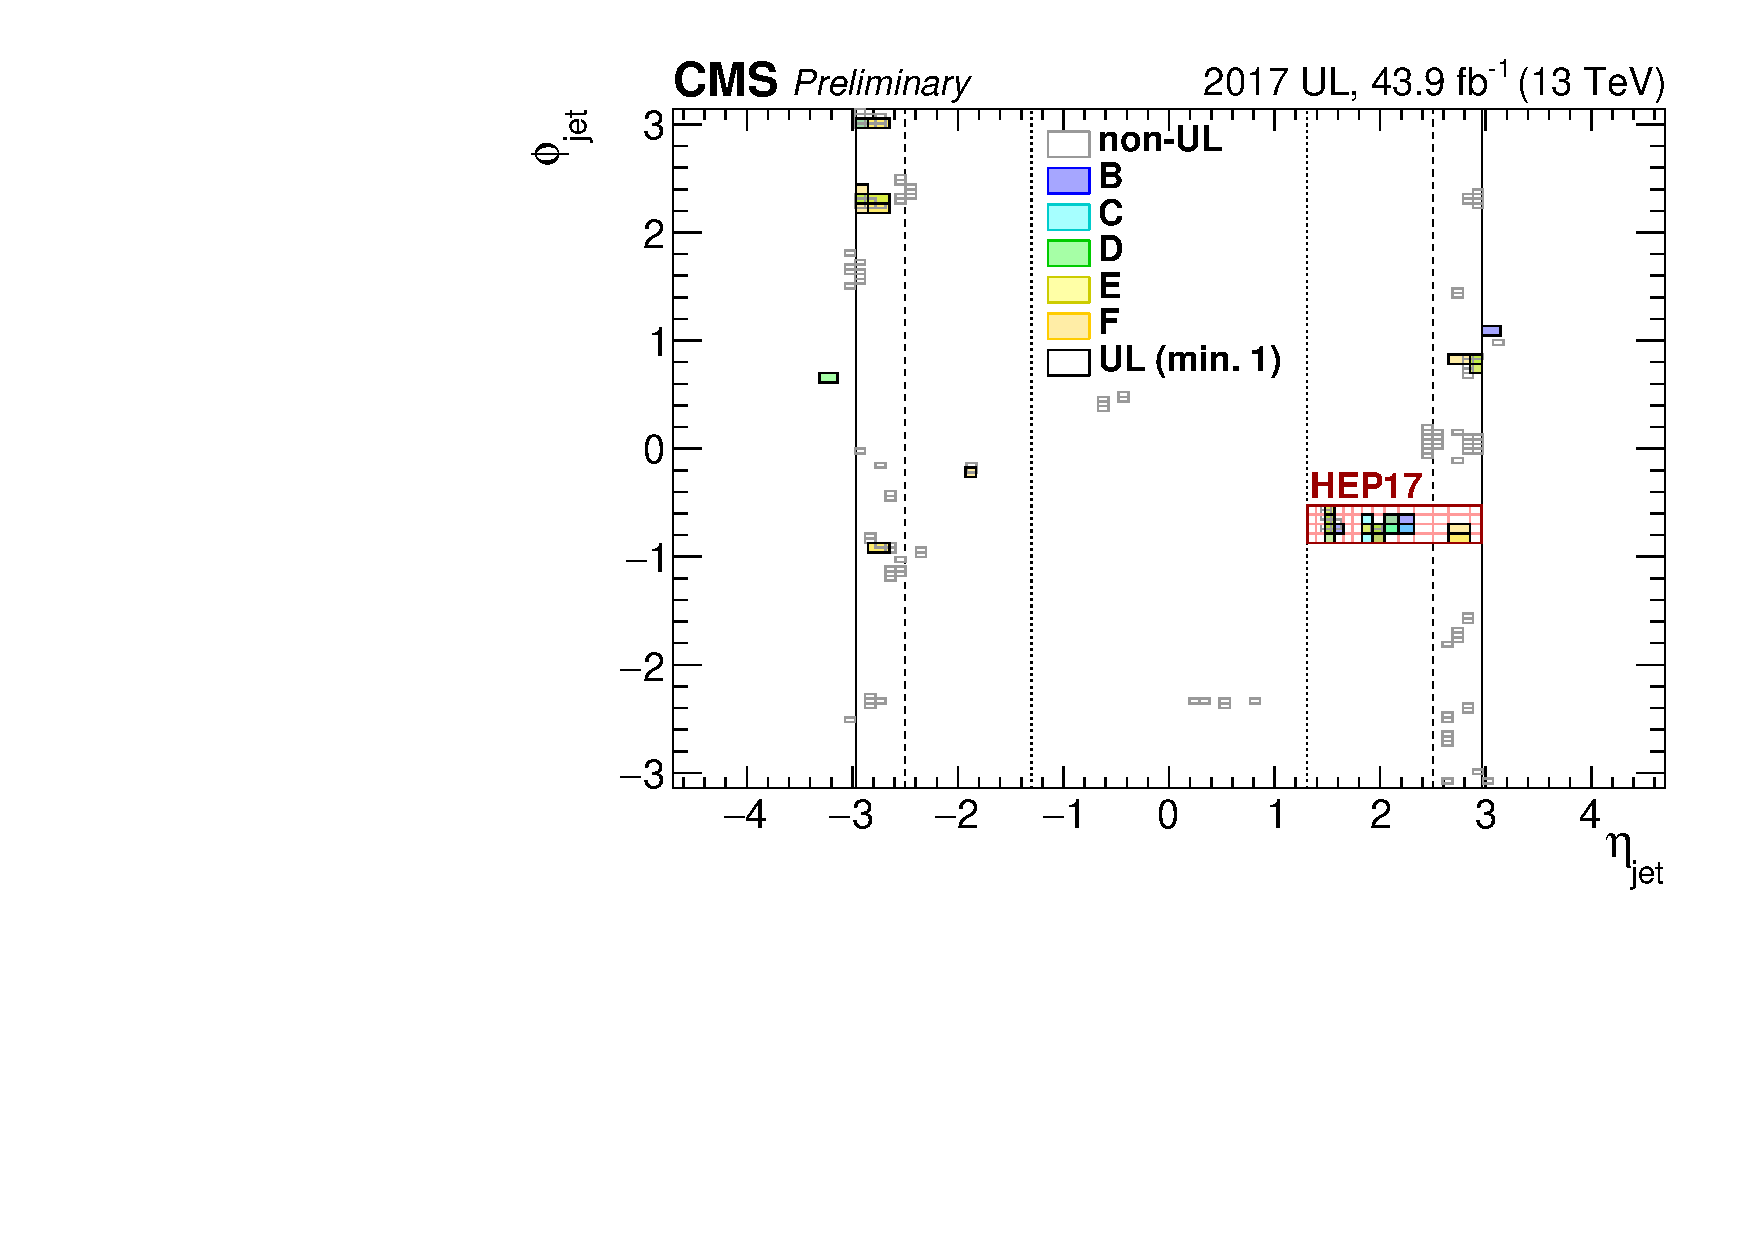
\includegraphics[width=.6\textwidth]{\PhDthesisdir/plots_and_images/hotjets2017UL.pdf}
\caption[Régions des calorimètres à exclure de l'analyse dans le plan $(\eta, \phi)$.]{Régions des calorimètres à exclure de l'analyse dans le plan $(\eta, \phi)$ pour les événements de 2017-UL. Certaines régions ne concernent que certaines périodes de l'année (en couleur). La région \og HEP17 \fg{} correspond à l'emplacement du système de lecture expérimental \og SiPM \fg~\cite{SiPM_CMS_conf}.}
\label{fig-hotjets2017UL}
\end{figure}
%Some regions of the calorimeters are observed to produce anomalously high jet rates. This phenomenon is understood to result from sub-optimal calorimeter calibration for jet measurement performance. We can eliminate any bias arising from the problematic detector regions by excluding events with important jets in the 'hot' calorimeter zones. Hot zone maps are available for the end-of-year (EOY) re-reconstructions for 2016-2018 and the Summer19UL17 reco version in the JECDatabase repository:
%
%https://github.com/cms-jet/JECDatabase/tree/master/hotzone_maps
%
%The EOY maps are there for archiving purposes and we don't have an official recommendation for them at the moment. In the UL17 directory there's two versions; with and without the entire HEP17 HCAL region with sub-optimal calibration resulting from the experimental SiPM read-out system. Our recommendation for UltraLegacy 17 processing is the following:
%
%    All JERC analysers and anybody doing precision measurements with jets should use the h2hot_ul17_plus_hep17 map
%    Searches that are sensitive to jet tails should use h2hot_ul17 for higher acceptance
%    Non-jet measurements and searches that are not sensitive to jet tails can either use h2hot17_ul17 or ignore these maps for highest acceptance
%    Please note that for analyses comparing data to simulation or otherwise relying heavily on simulation, it may be necessary to use the filtering also for MC processing for ensuring avoiding any biases due to angular dependencies etc. In these cases the same data-based filter should be used for data and MC. The maps labelled 'mc' (=pythia) or 'hw' (=herwig) in the JECDatabase are for expert studies only. 
\paragraph{Sélection sur le chemin de déclenchement}
Comme expliqué dans la section~\ifref{chapter-LHC-section-CMS-subsec-data_taking}{\ref{chapter-LHC-section-CMS-subsec-data_taking}}{2.7} du chapitre~\ifref{chapter-LHC}{\ref{chapter-LHC}}{3}, un événement observé par le détecteur CMS est sauvegardé si un chemin de déclenchement est activé.
Dans cette analyse, seuls les événements dont le photon servant d'objet de référence pour la calibration des jets correspond au photon ayant activé le chemin de déclenchement pour cet événement sont retenus.
Or, plus l'impulsion transverse du photon est faible, plus le nombre d'événements pouvant être sauvegardés est importante, si bien que la chaîne d'acquisition arrive à saturation.
Pour pallier à cette saturation, il existe différents chemins de déclenchement en fonction de l'impulsion transverse du photon et pour chacun d'entre eux, seule une fraction des événements les déclenchant est effectivement sauvegardée.
Cette fraction est nommée \emph{prescale}.
À chaque chemin de déclenchement correspond ainsi un \emph{prescale}.
Un intervalle d'impulsion transverse du photon retenu est alors défini pour chaque chemin de déclenchement utilisé.
Cet intervalle permet de se placer au plateau d'efficacité du chemin de déclenchement.
Les différents chemins de déclenchement, leurs \emph{prescales} et intervalles d'impulsion transverse sont présentés dans le tableau~\ref{tab-HLT_pT_precales_18_and_17UL}.
Par exemple, un photon d'impulsion transverse \SI{95}{\GeV} doit avoir déclenché le chemin nommé \inlinecode{python}{HLT_Photon75_R9Id90_HE10_IsoM}.
\begin{table}[h]
\centering
\begin{tabular}{lccc}
\toprule
Chemin de déclenchement & $\pT^{\photon}$ (\SI{}{\GeV}) & \emph{Prescale} 2018 & \emph{Prescale} 2017-UL\\
\midrule
%\inlinecode{python}{HLT_Photon33} & $[\num{40}, \num{60}[$ & \num{4.0115375867e-5} & \num{3.434860938821936e-4} \\
%\inlinecode{python}{HLT_Photon50_R9Id90_HE10_IsoM} & $[\num{60}, \num{85}[$ & \num{3.9473720141e-3} & \num{7.40465688874224e-3} \\
%\inlinecode{python}{HLT_Photon75_R9Id90_HE10_IsoM} & $[\num{85}, \num{105}[$ & \num{0.0156656382257} & \num{0.03195516364518142} \\
%\inlinecode{python}{HLT_Photon90_R9Id90_HE10_IsoM} & $[\num{105}, \num{130}[$ & \num{0.0312899931745} & \num{0.0636323095006467} \\
%\inlinecode{python}{HLT_Photon120_R9Id90_HE10_IsoM} & $[\num{130}, \num{175}[$ & \num{0.125036122867} & \num{0.18787162142132302} \\
%\inlinecode{python}{HLT_Photon165_R9Id90_HE10_IsoM} & $[\num{175}, \num{230}[$ & \num{0.250030962458} & \num{0.6823580953102895} \\
%\inlinecode{python}{HLT_Photon200} & $[\num{230}, +\infty$ & \num{1} & \num{1} \\
\inlinecode{python}{HLT_Photon33} & $[\num{40}, \num{60}[$ & \num{4.01154e-5} & \num{3.43486e-4} \\
\inlinecode{python}{HLT_Photon50_R9Id90_HE10_IsoM} & $[\num{60}, \num{85}[$ & \num{3.94737e-3} & \num{7.40466e-3} \\
\inlinecode{python}{HLT_Photon75_R9Id90_HE10_IsoM} & $[\num{85}, \num{105}[$ & \num{0.0156656} & \num{0.0319552} \\
\inlinecode{python}{HLT_Photon90_R9Id90_HE10_IsoM} & $[\num{105}, \num{130}[$ & \num{0.0312900} & \num{0.0636323} \\
\inlinecode{python}{HLT_Photon120_R9Id90_HE10_IsoM} & $[\num{130}, \num{175}[$ & \num{0.125036} & \num{0.187872} \\
\inlinecode{python}{HLT_Photon165_R9Id90_HE10_IsoM} & $[\num{175}, \num{230}[$ & \num{0.250031} & \num{0.682358} \\
\inlinecode{python}{HLT_Photon200} & $[\num{230}, +\infty [$ & \num{1} & \num{1} \\
\bottomrule
\end{tabular}
\caption[Chemins de déclenchement.]{Chemins de déclenchement, intervalles d'impulsion transverse du photon et \emph{prescales} utilisés.}
\label{tab-HLT_pT_precales_18_and_17UL}
\end{table}
\subsection{Analyse}\label{chapter-JERC-section-JES-subsec-analyse}
\paragraph{Intervalles de $\pT^{\photon}$}
L'analyse a pour but de déterminer la correction résiduelle absolue en \pT\ des jets, définie dans la section~\ref{chapter-JERC-section-CMS-subsec-residuals}.
Pour cela, l'écart à l'unité du rapport moyen des réponses des jets dans les données et les simulations est déterminé dans différents intervalles de $\pT^{\photon}$, listés dans le tableau~\ref{tab-pT_photon_intervalles}.
Ils sont une subdivision des intervalles définis pour les chemin de déclenchement dans le tableau~\ref{tab-HLT_pT_precales_18_and_17UL}, ce qui permet de séparer le traitement des événements correspondant à différents chemins de déclenchement.
\begin{table}[h]
\centering
\begin{tabular}{cccc}
\toprule
$[\num{40}, \num{50}[$ & $[\num{50}, \num{60}[$ & $[\num{60}, \num{85}[$ & $[\num{85}, \num{105}[$ \\
$[\num{105}, \num{130}[$ & $[\num{130}, \num{175}[$ & $[\num{175}, \num{230}[$ & $[\num{230}, \num{300}[$ \\
$[\num{300}, \num{400}[$ & $[\num{400}, \num{500}[$ & $[\num{500}, \num{700}[$ & $[\num{700}, \num{1000}[$ \\
$[\num{1000}, \num{3000}]$ \\
\bottomrule
\end{tabular}
\caption[Intervalles de $\pT^{\photon}$.]{Intervalles de $\pT^{\photon}$ en \SI{}{\GeV}.}
\label{tab-pT_photon_intervalles}
\end{table}
\paragraph{Intervalles de $\abs{\eta^\text{jet}}$}
La calibration en énergie des jets dépend fortement de la région du détecteur dans laquelle le jet laisse un signal, comme le montre la figure~\ref{fig-simulated_jet_response_RunII} en page~\pageref{fig-simulated_jet_response_RunII}.
Cet effet est dû aux différentes technologies utilisées ainsi qu'au vieillissement non uniforme du détecteur.
Des intervalles de pseudo-rapidité du jet sont ainsi définis dans le tableau~\ref{tab-eta_jet_intervalles_large} afin de séparer le traitement de ces différentes régions.
\begin{table}[h]
\centering
\begin{tabular}{cccc}
\toprule
$[\num{0}\isp \num{0.783}[$ & $[\num{0.783}\isp \num{1.305}[$ & $[\num{1.305}\isp \num{1.93}[$ & $[\num{1.93}\isp \num{2.5}[$ \\
$[\num{2.5}\isp \num{2.964}[$ & $[\num{2.964}\isp \num{3.2}[$ & $[\num{3.2}\isp \num{5.191}[$ &  \\
\bottomrule
\end{tabular}
\caption{Intervalles larges de $\abs{\eta^\text{jet}}$.}
\label{tab-eta_jet_intervalles_large}
\end{table}
%\begin{table}[h]
%\centering
%\begin{tabular}{cccccc}
%\toprule
%$[\num{0}\isp \num{0.261}[$ & $[\num{0.261}\isp \num{0.522}[$ & $[\num{0.522}\isp \num{0.783}[$ & $[\num{0.783}\isp \num{1.044}[$ & $[\num{1.044}\isp \num{1.305}[$ & $[\num{1.305}\isp \num{1.479}[$ \\
%$[\num{1.479}\isp \num{1.653}[$ & $[\num{1.653}\isp \num{1.930}[$ & $[\num{1.930}\isp \num{2.172}[$ & $[\num{2.172}\isp \num{2.322}[$ & $[\num{2.322}\isp \num{2.500}[$ & $[\num{2.500}\isp \num{2.650}[$ \\
%$[\num{2.650}\isp \num{2.853}[$ & $[\num{2.853}\isp \num{2.964}[$ & $[\num{2.964}\isp \num{3.319}[$ & $[\num{3.319}\isp \num{3.489}[$ & $[\num{3.489}\isp \num{3.839}[$ & $[\num{3.839}\isp \num{5.191}[$ \\
%\bottomrule
%\end{tabular}
%\caption{Intervalles fins de $\abs{\eta^\text{jet}}$.}
%\label{tab-eta_jet_intervalles_fin}
%\end{table}
\paragraph{Pondération par l'empilement}
Le profil d'empilement, \ie\ la densité de probabilité du nombre d'interactions d'empilement, dépend de la période de la prise de données et du chemin de déclenchement par lequel l'événement est retenu. Ces dépendances sont illustrées sur les graphiques des figures~\ref{fig-PU_profile_18} et~\ref{fig-PU_profile_17UL}.
Les événements simulés sont ainsi pondérés pour faire correspondre leur profil d'empilement à celui des données, en prenant en compte la double dépendance avec la période de prise de donnée et le chemin de déclenchement.
\begin{figure}[p]
\centering
\subcaptionbox{Run 2018 A.\label{subfig-PU_profile_18_A}}[.45\textwidth]
{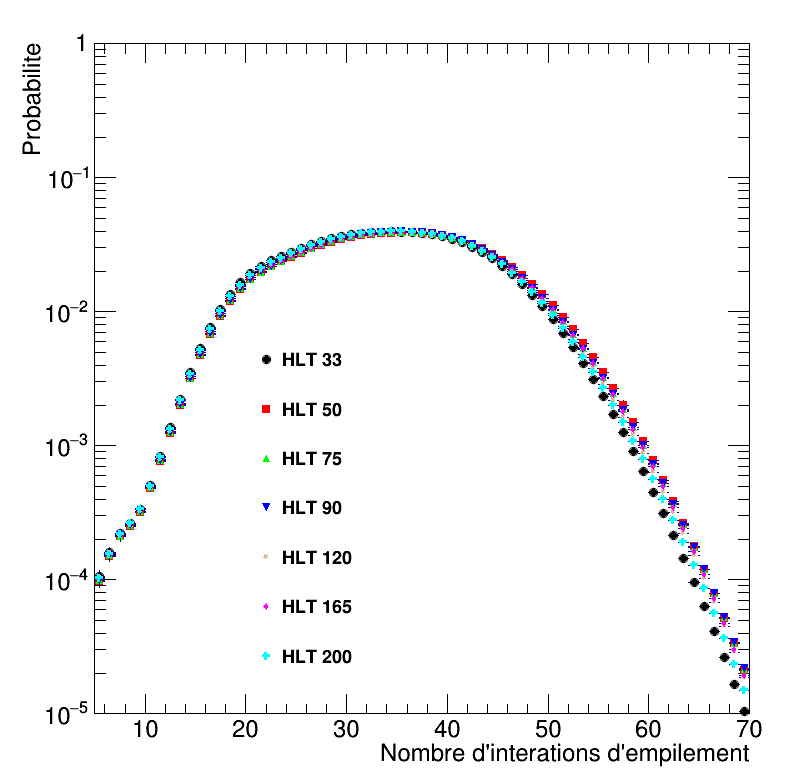
\includegraphics[width=.45\textwidth]{\PhDthesisdir/plots_and_images/my_plots/JERC/PUreweighting/2018/with_header/PU_HLT_profiles_run2018A_only_L2Res.tex}\vspace{-.5\baselineskip}}
\hfill
\subcaptionbox{Run 2018 B.\label{subfig-PU_profile_18_B}}[.45\textwidth]
{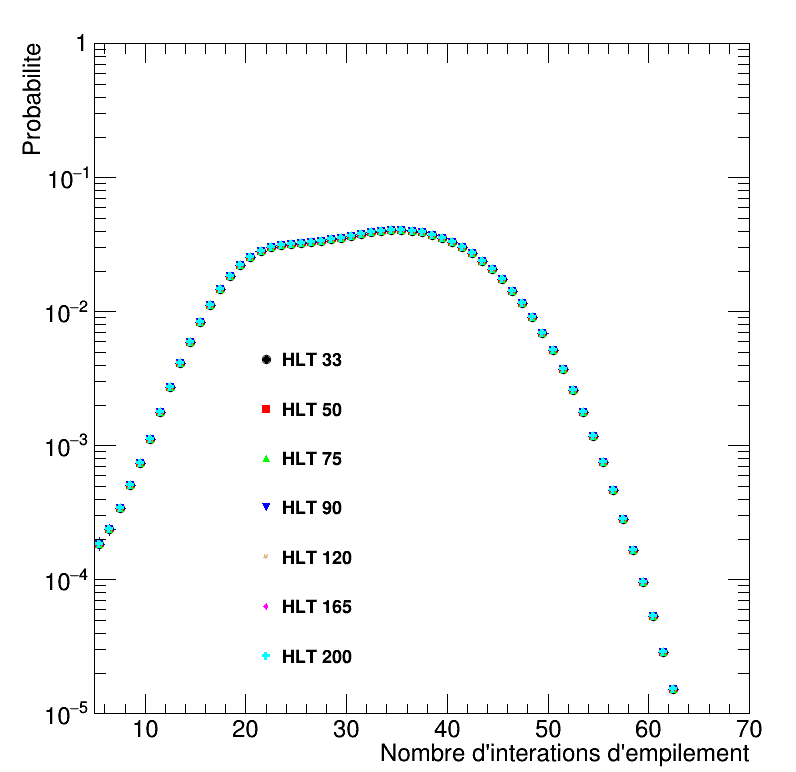
\includegraphics[width=.45\textwidth]{\PhDthesisdir/plots_and_images/my_plots/JERC/PUreweighting/2018/with_header/PU_HLT_profiles_run2018B_only_L2Res.tex}\vspace{-.5\baselineskip}}

\vspace{.75\baselineskip}

\subcaptionbox{Run 2018 C.\label{subfig-PU_profile_18_C}}[.45\textwidth]
{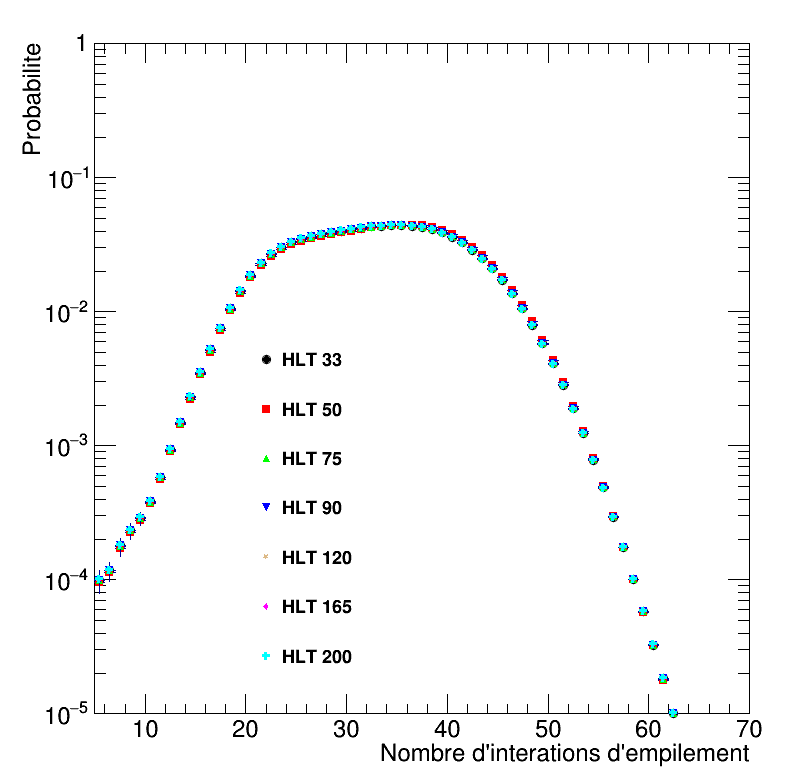
\includegraphics[width=.45\textwidth]{\PhDthesisdir/plots_and_images/my_plots/JERC/PUreweighting/2018/with_header/PU_HLT_profiles_run2018C_only_L2Res.tex}\vspace{-.5\baselineskip}}
\hfill
\subcaptionbox{Run 2018 D.\label{subfig-PU_profile_18_D}}[.45\textwidth]
{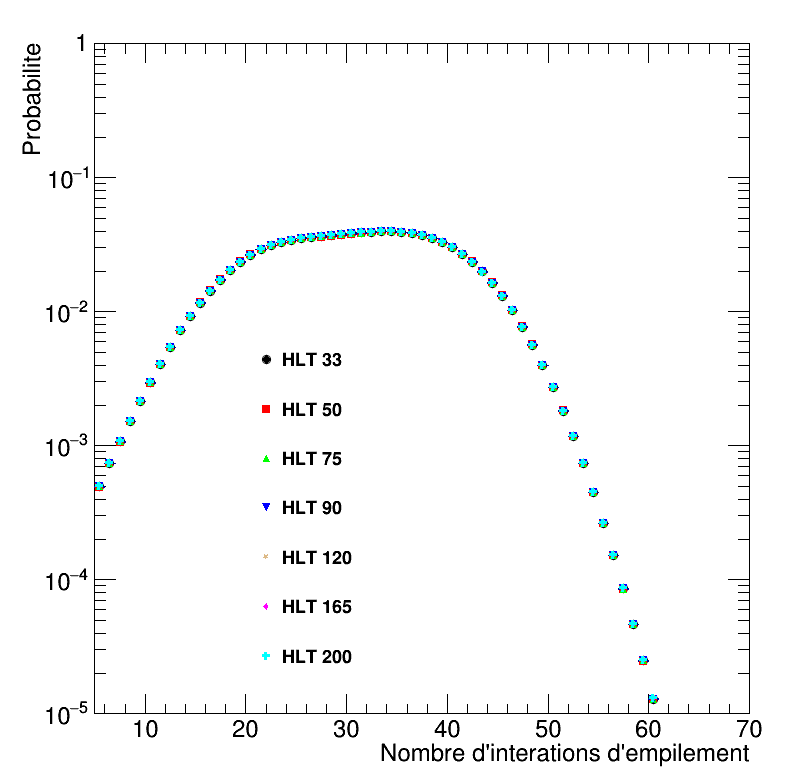
\includegraphics[width=.45\textwidth]{\PhDthesisdir/plots_and_images/my_plots/JERC/PUreweighting/2018/with_header/PU_HLT_profiles_run2018D_only_L2Res.tex}\vspace{-.5\baselineskip}}

\vspace{.75\baselineskip}

\subcaptionbox{Run 2018 ABC.\label{subfig-PU_profile_18_ABC}}[.45\textwidth]
{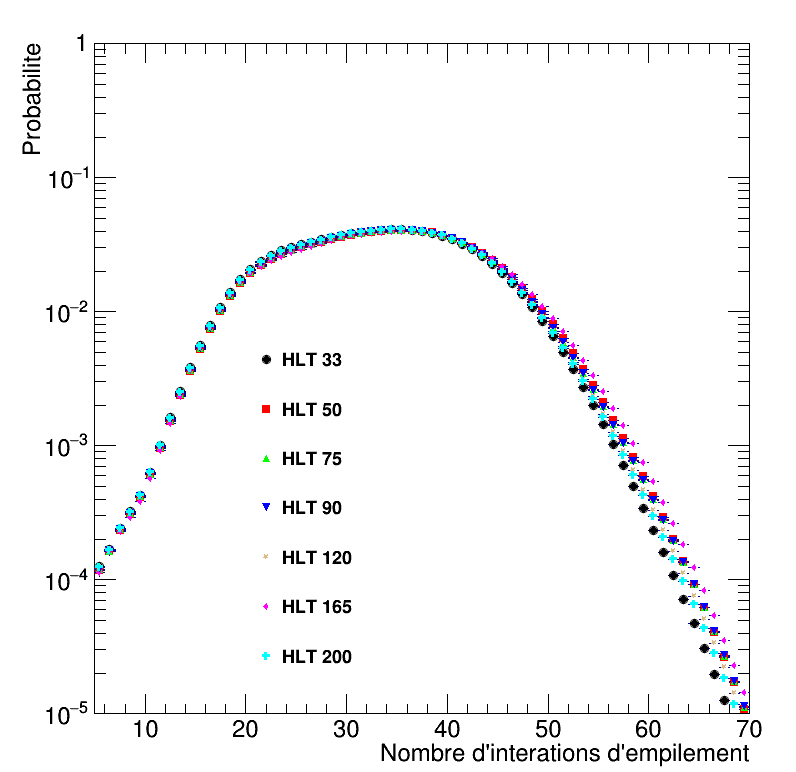
\includegraphics[width=.45\textwidth]{\PhDthesisdir/plots_and_images/my_plots/JERC/PUreweighting/2018/with_header/PU_HLT_profiles_run2018ABC_only_L2Res.tex}\vspace{-.5\baselineskip}}
\hfill
\subcaptionbox{Run 2018 ABCD.\label{subfig-PU_profile_18_ABCD}}[.45\textwidth]
{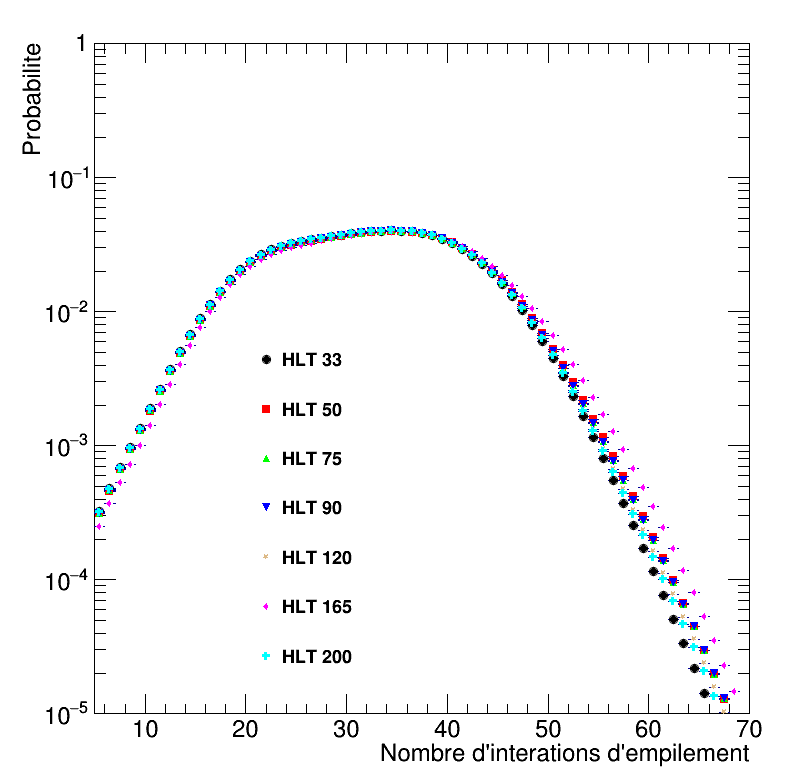
\includegraphics[width=.45\textwidth]{\PhDthesisdir/plots_and_images/my_plots/JERC/PUreweighting/2018/with_header/PU_HLT_profiles_run2018ABCD_only_L2Res.tex}\vspace{-.5\baselineskip}}

\caption[Densités de probabilité de $N_\text{PU}$ pour 2018.]{Densités de probabilité du nombre d'interactions d'empilement $N_\text{PU}$ pour les périodes de prises de données de 2018.}
\label{fig-PU_profile_18}
\end{figure}
\begin{figure}[p]
\centering
\subcaptionbox{Run 2017-UL B.\label{subfig-PU_profile_17UL_B}}[.45\textwidth]
{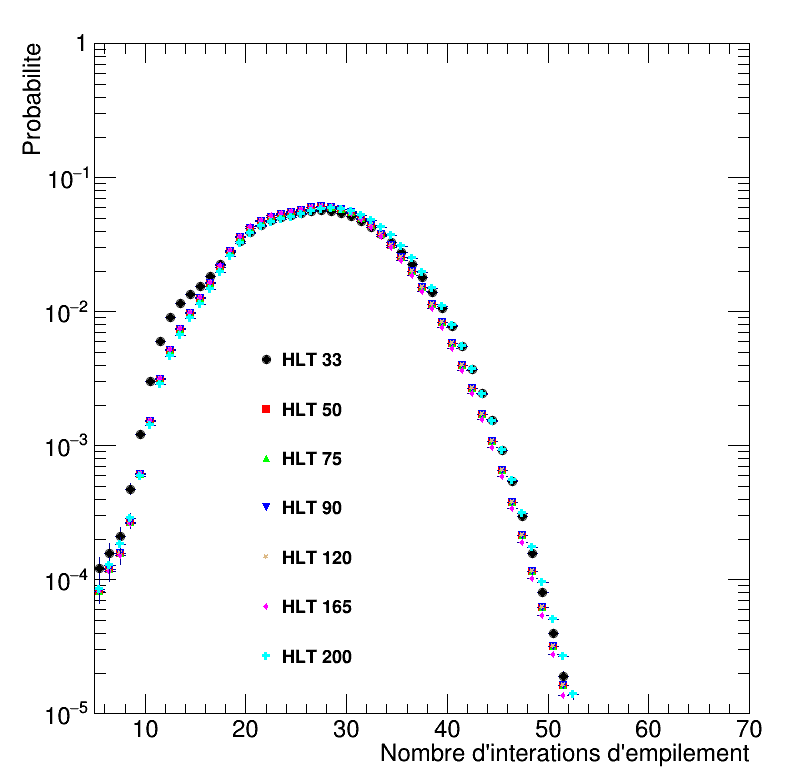
\includegraphics[width=.45\textwidth]{\PhDthesisdir/plots_and_images/my_plots/JERC/PUreweighting/2017UL/with_header/PU_HLT_profiles_run2017B_only_L2Res.tex}\vspace{-.5\baselineskip}}
\hfill
\subcaptionbox{Run 2017-UL C.\label{subfig-PU_profile_17UL_C}}[.45\textwidth]
{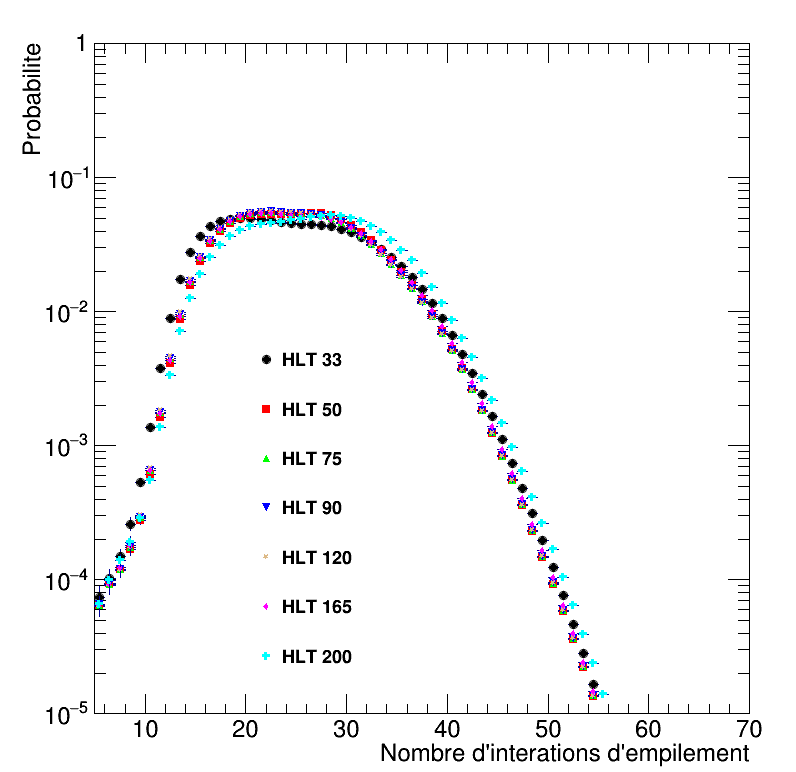
\includegraphics[width=.45\textwidth]{\PhDthesisdir/plots_and_images/my_plots/JERC/PUreweighting/2017UL/with_header/PU_HLT_profiles_run2017C_only_L2Res.tex}\vspace{-.5\baselineskip}}

\vspace{.75\baselineskip}

\subcaptionbox{Run 2017-UL D.\label{subfig-PU_profile_17UL_D}}[.45\textwidth]
{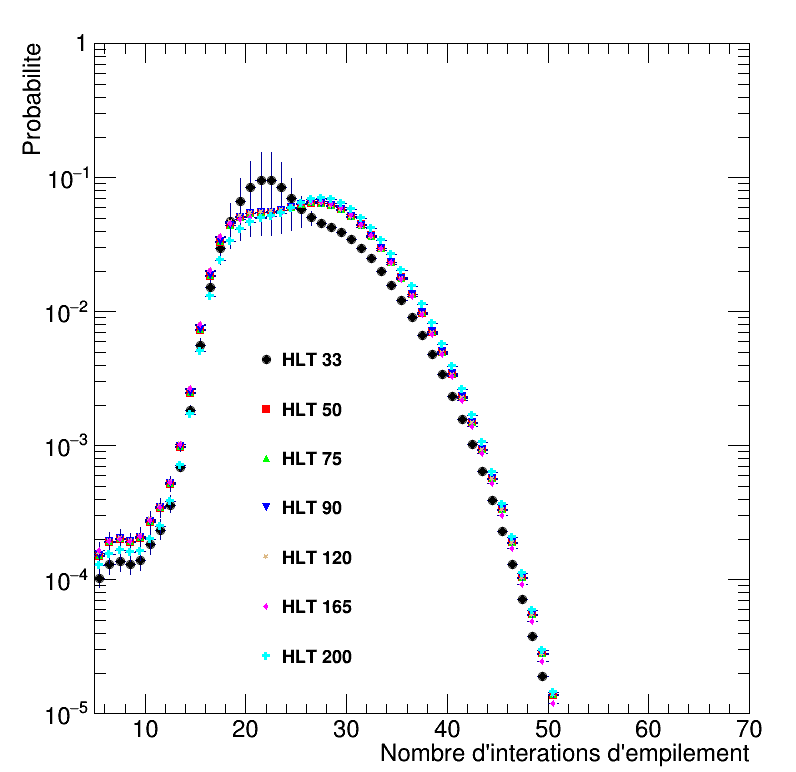
\includegraphics[width=.45\textwidth]{\PhDthesisdir/plots_and_images/my_plots/JERC/PUreweighting/2017UL/with_header/PU_HLT_profiles_run2017D_only_L2Res.tex}\vspace{-.5\baselineskip}}
\hfill
\subcaptionbox{Run 2017-UL E.\label{subfig-PU_profile_17UL_E}}[.45\textwidth]
{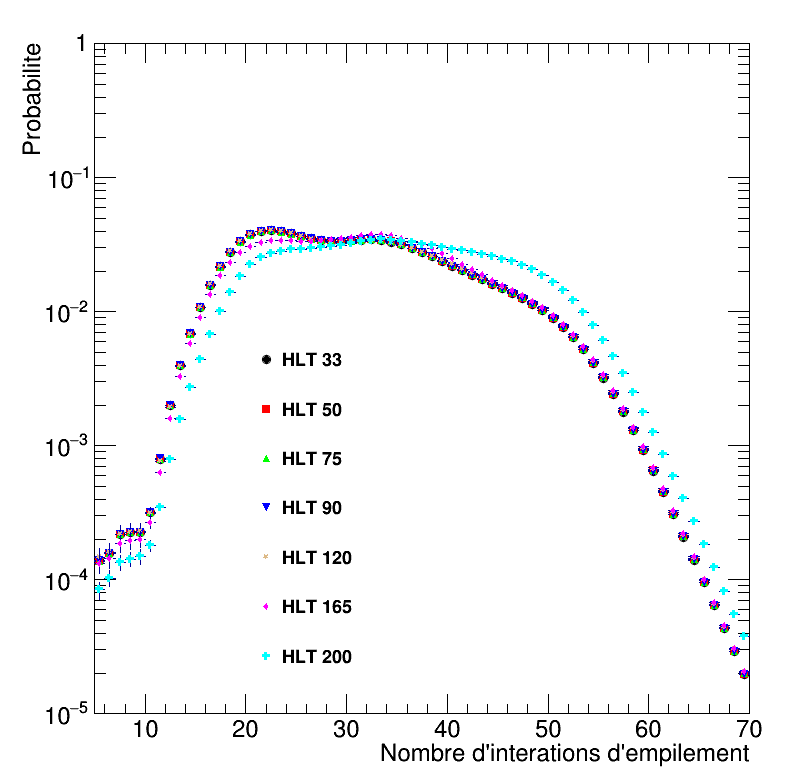
\includegraphics[width=.45\textwidth]{\PhDthesisdir/plots_and_images/my_plots/JERC/PUreweighting/2017UL/with_header/PU_HLT_profiles_run2017E_only_L2Res.tex}\vspace{-.5\baselineskip}}

\vspace{.75\baselineskip}

\subcaptionbox{Run 2017-UL F.\label{subfig-PU_profile_17UL_F}}[.45\textwidth]
{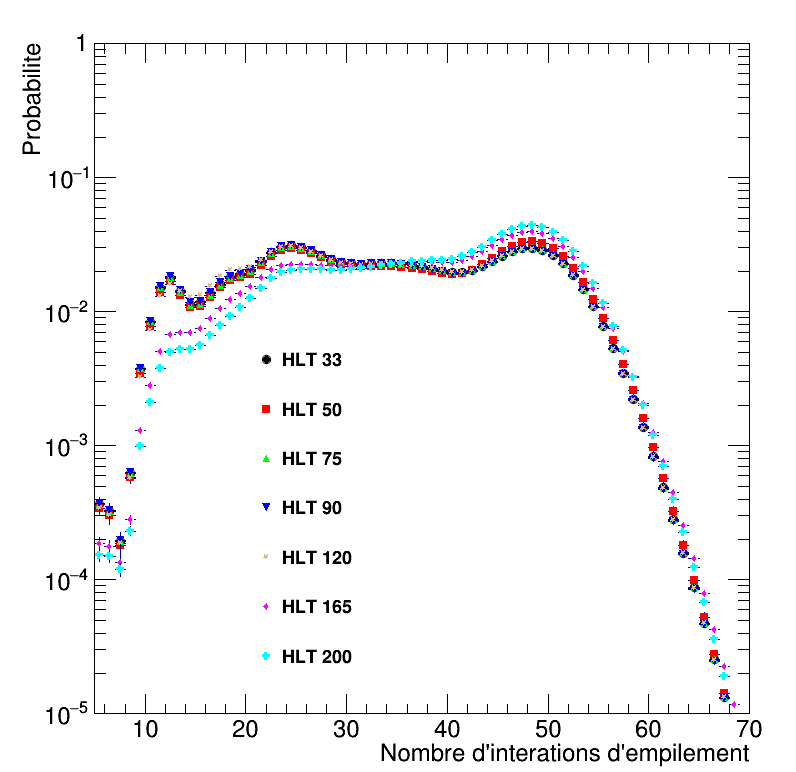
\includegraphics[width=.45\textwidth]{\PhDthesisdir/plots_and_images/my_plots/JERC/PUreweighting/2017UL/with_header/PU_HLT_profiles_run2017F_only_L2Res.tex}\vspace{-.5\baselineskip}}
\hfill
\subcaptionbox{Run 2017-UL BCDEF.\label{subfig-PU_profile_17UL_BCDEF}}[.45\textwidth]
{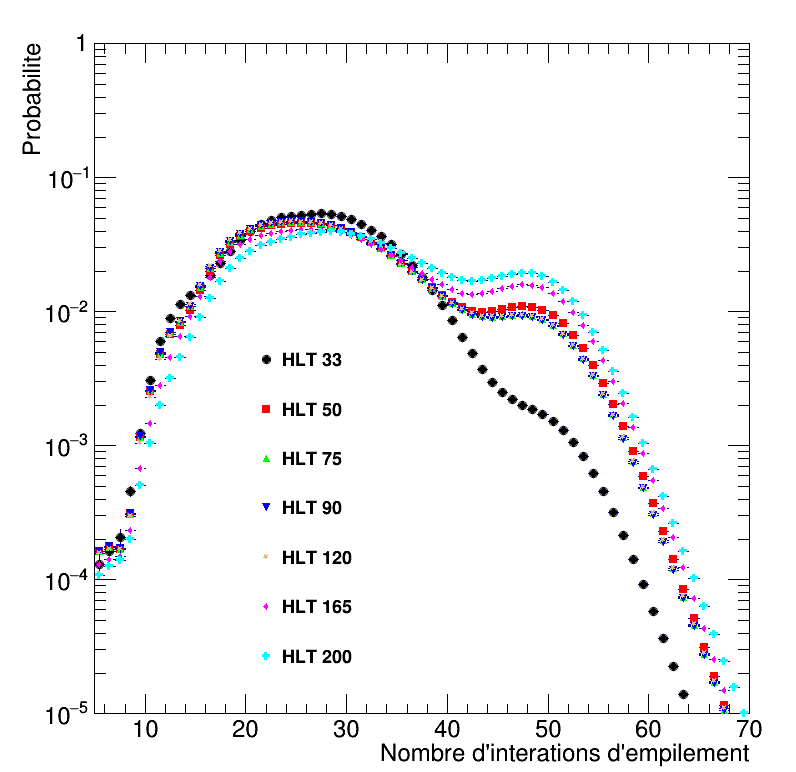
\includegraphics[width=.45\textwidth]{\PhDthesisdir/plots_and_images/my_plots/JERC/PUreweighting/2017UL/with_header/PU_HLT_profiles_run2017BCDEF_only_L2Res.tex}\vspace{-.5\baselineskip}}

\caption[Densités de probabilité de $N_\text{PU}$ pour 2017-UL.]{Densités de probabilité du nombre d'interactions d'empilement $N_\text{PU}$ pour les périodes de prises de données de 2017-UL.}
\label{fig-PU_profile_17UL}
\end{figure}
\paragraph{Accord données-simulations}
Pour comparer les distributions des observables dans les événements, les distributions des événements simulés sont normalisées à la luminosité mesurée pour le jeu de données considéré.
Les comparaisons étant faites entre les données et les événements simulés \Gjets, un désaccord dû à la contamination à bas \pT\ d'événements multijet est attendu, ces événements n'étant pas présents dans les simulations utilisées.
De plus, l'utilisation d'une simulation au premier ordre perturbatif seulement influe sur le nombre de jets dans l'état final qui s'en trouve plus faible, en particulier dans les queues des distributions.
Ces désaccords se constatent sur les graphiques de la figure~\ref{fig-distribs_Gjets_18} présentant les distributions de l'impulsion transverse du photon, l'énergie transverse manquante et les impulsions transverses du premier et du second jet.
Afin de déterminer la correction résiduelle absolue en \pT\ des jets ainsi que la correction de leur résolution en énergie, seule la comparaison des distributions de \Rbal\ et \RMPF\ est nécessaire.
L'accord ainsi obtenu entre données et simulations est considéré comme suffisant.
\begin{figure}[h]
\centering
\subcaptionbox{Impulsion transverse du photon.\label{subfig-distrib_Gjets_18_ptPhoton}}[.45\textwidth]
{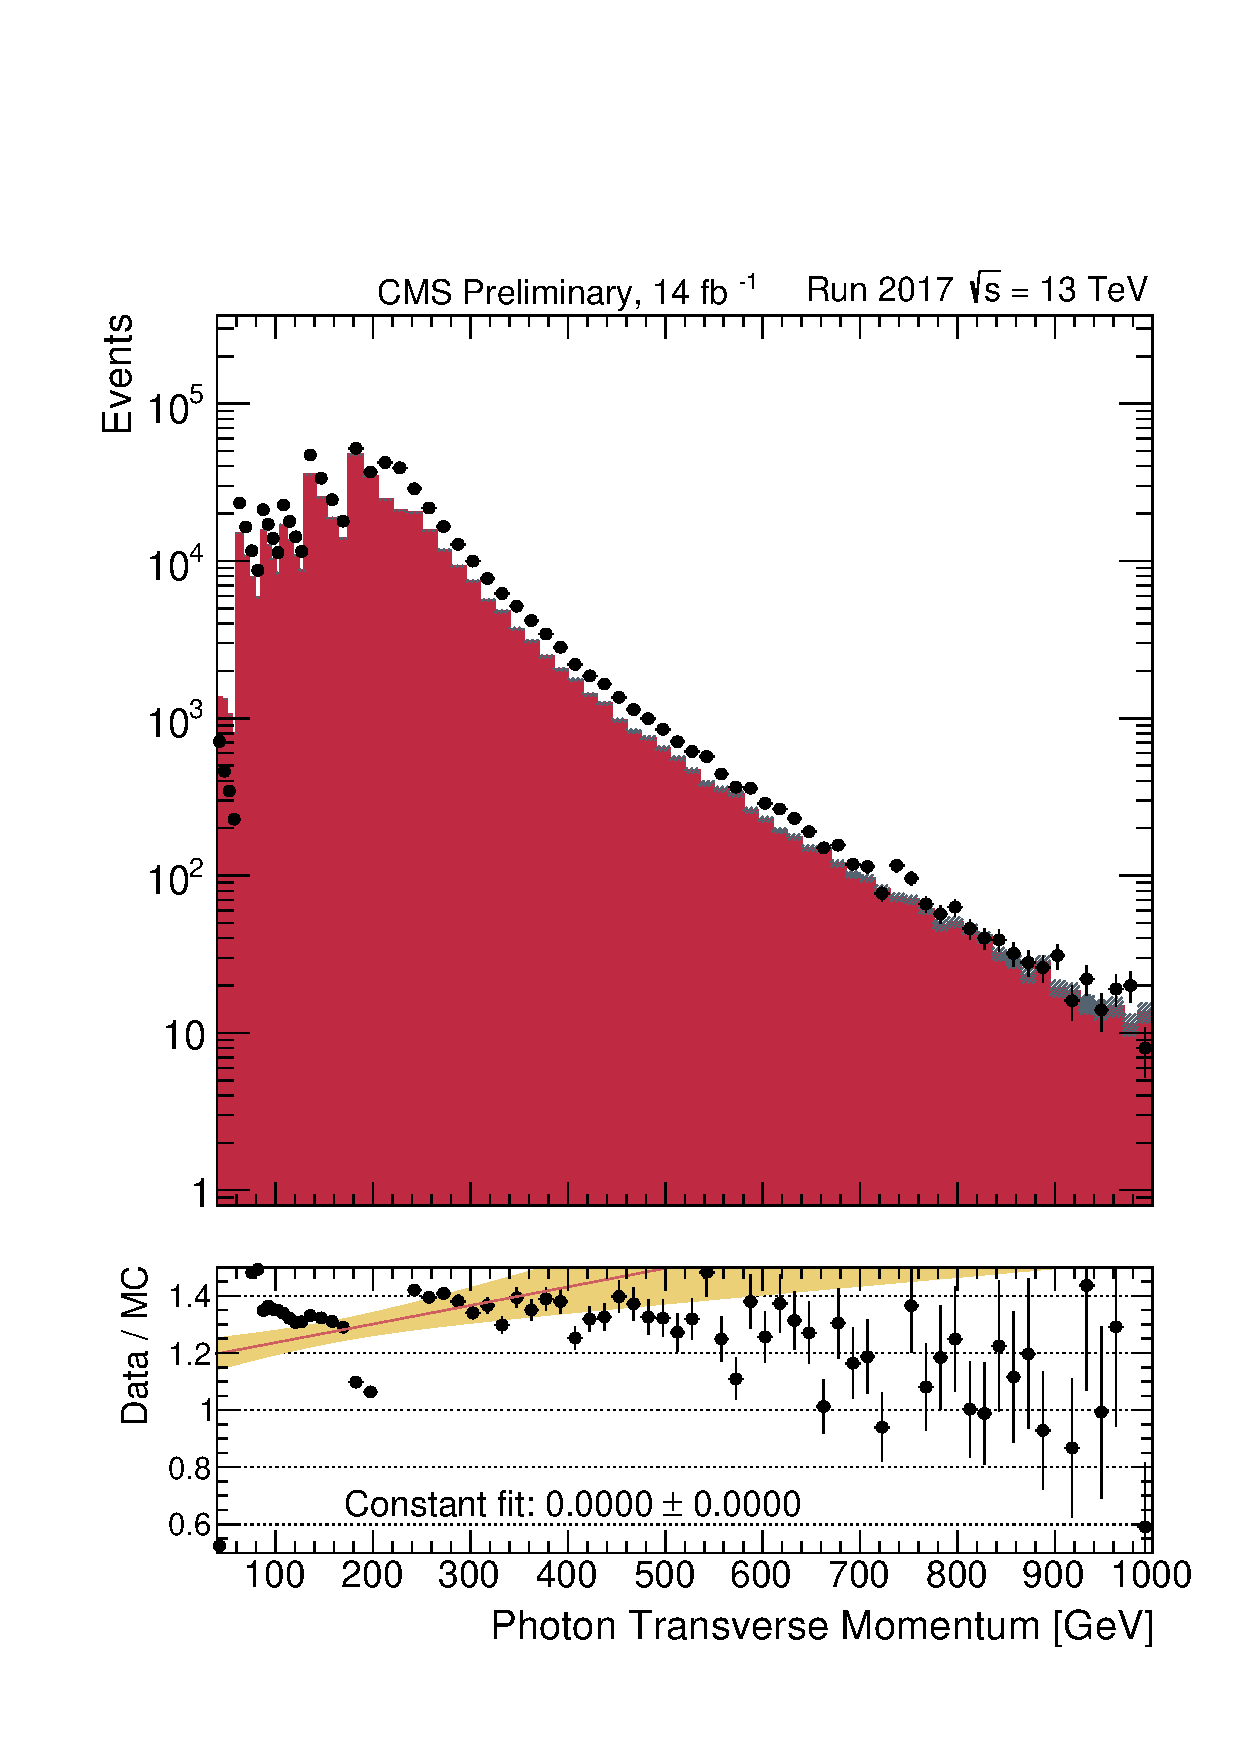
\includegraphics[width=.45\textwidth]{\PhDthesisdir/plots_and_images/my_plots/JERC/distributions/2018/with_header/ptPhoton_log.tex}}
\hfill
\subcaptionbox{Énergie transverse manquante.\label{subfig-distrib_Gjets_18_MET}}[.45\textwidth]
{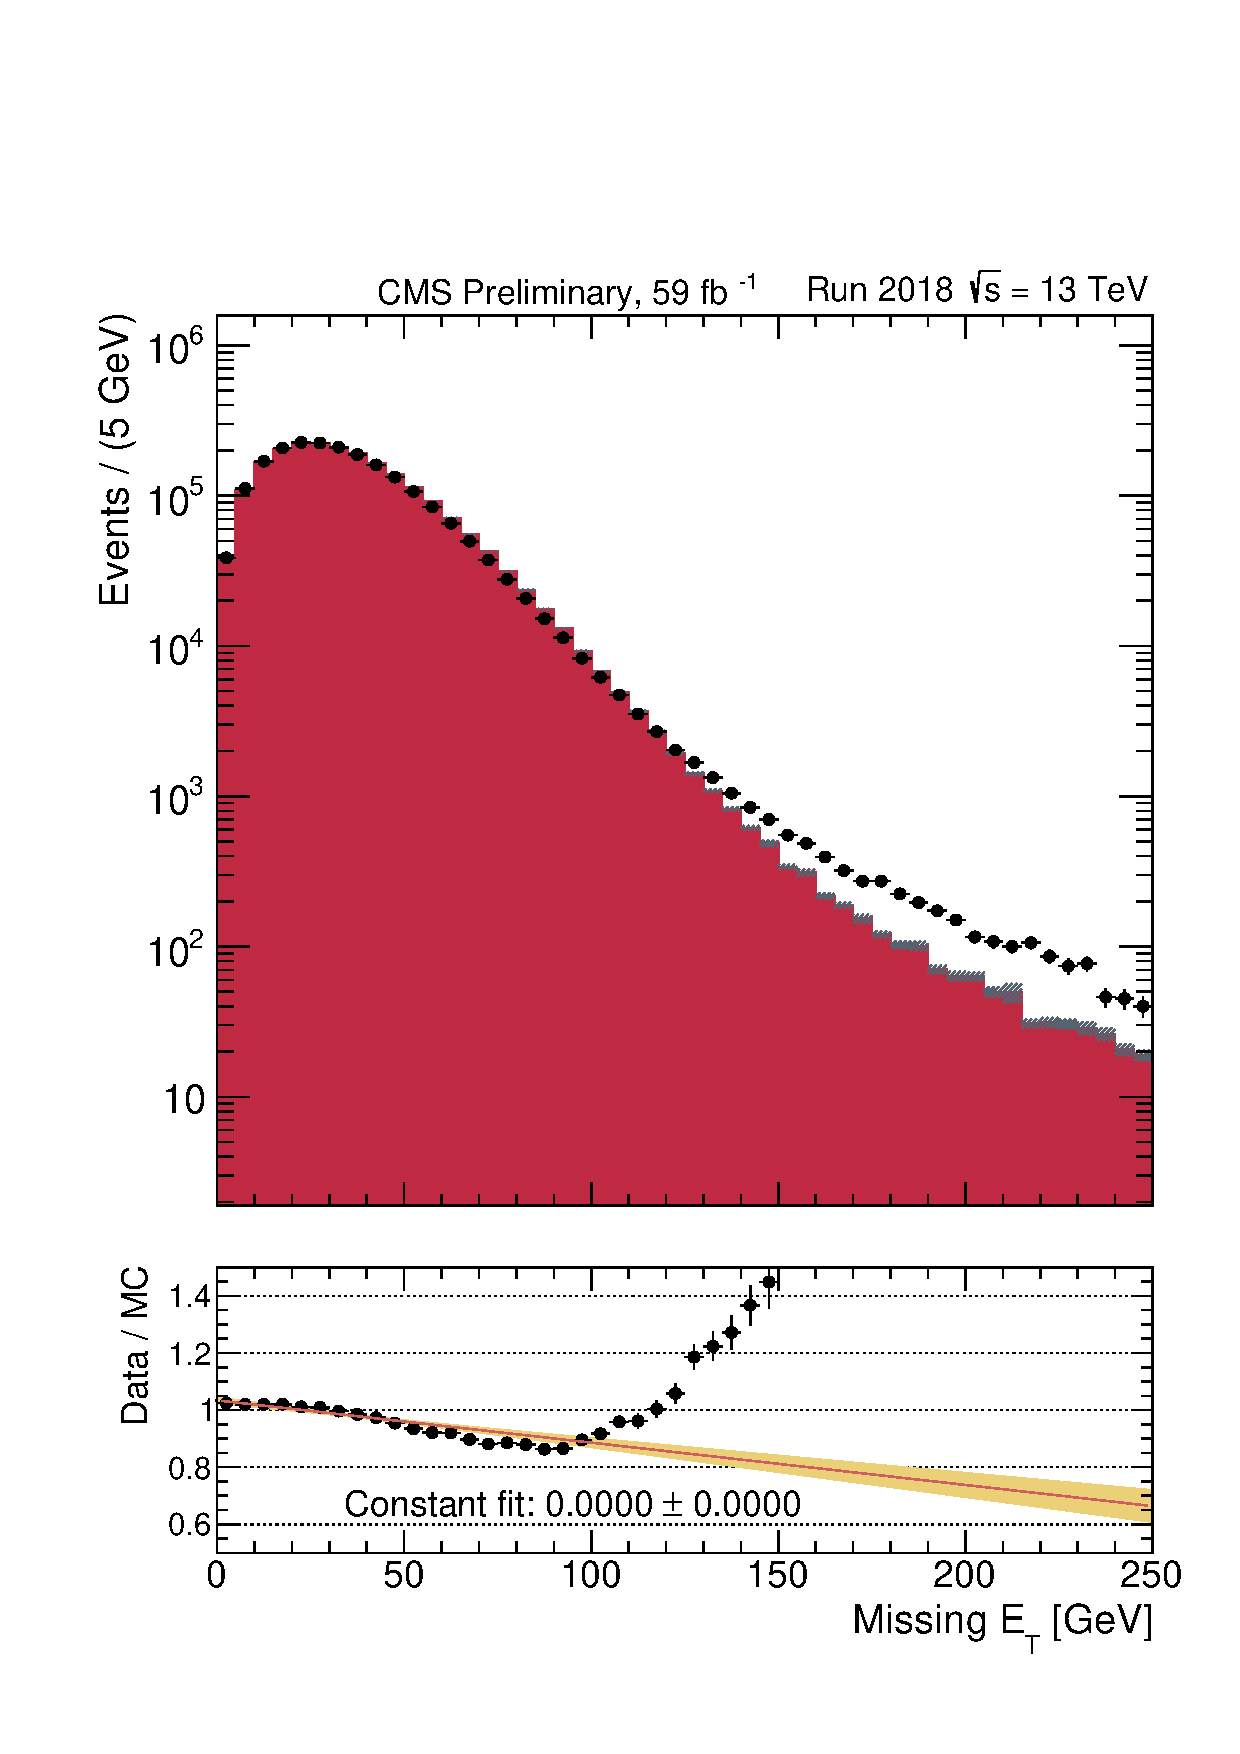
\includegraphics[width=.45\textwidth]{\PhDthesisdir/plots_and_images/my_plots/JERC/distributions/2018/with_header/MET_log.tex}}

\vspace{\baselineskip}

\subcaptionbox{Impulsion transverse du premier jet.\label{subfig-distrib_Gjets_18_ptFirstJet}}[.45\textwidth]
{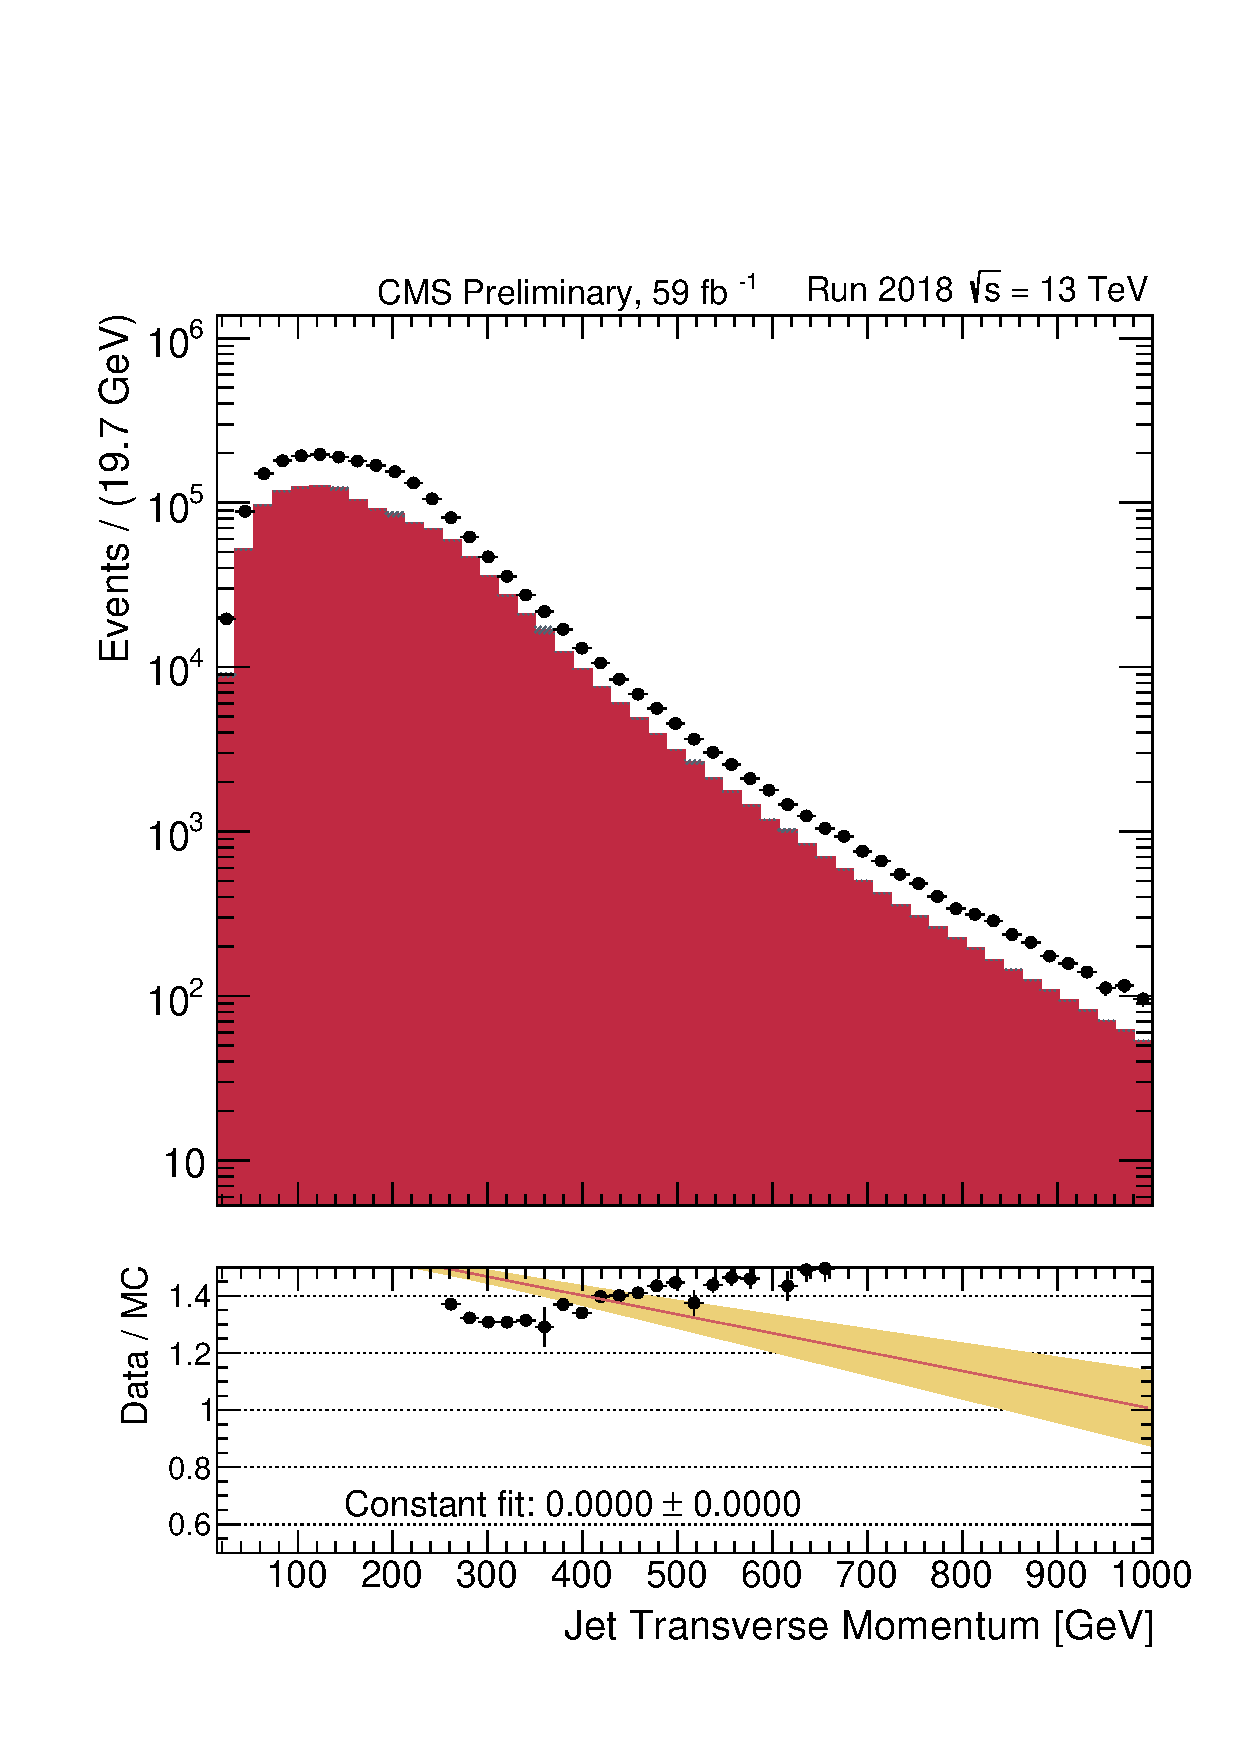
\includegraphics[width=.45\textwidth]{\PhDthesisdir/plots_and_images/my_plots/JERC/distributions/2018/with_header/ptFirstJet_log.tex}}
\hfill
\subcaptionbox{Impulsion transverse du second jet.\label{subfig-distrib_Gjets_18_ptSecondJet}}[.45\textwidth]
{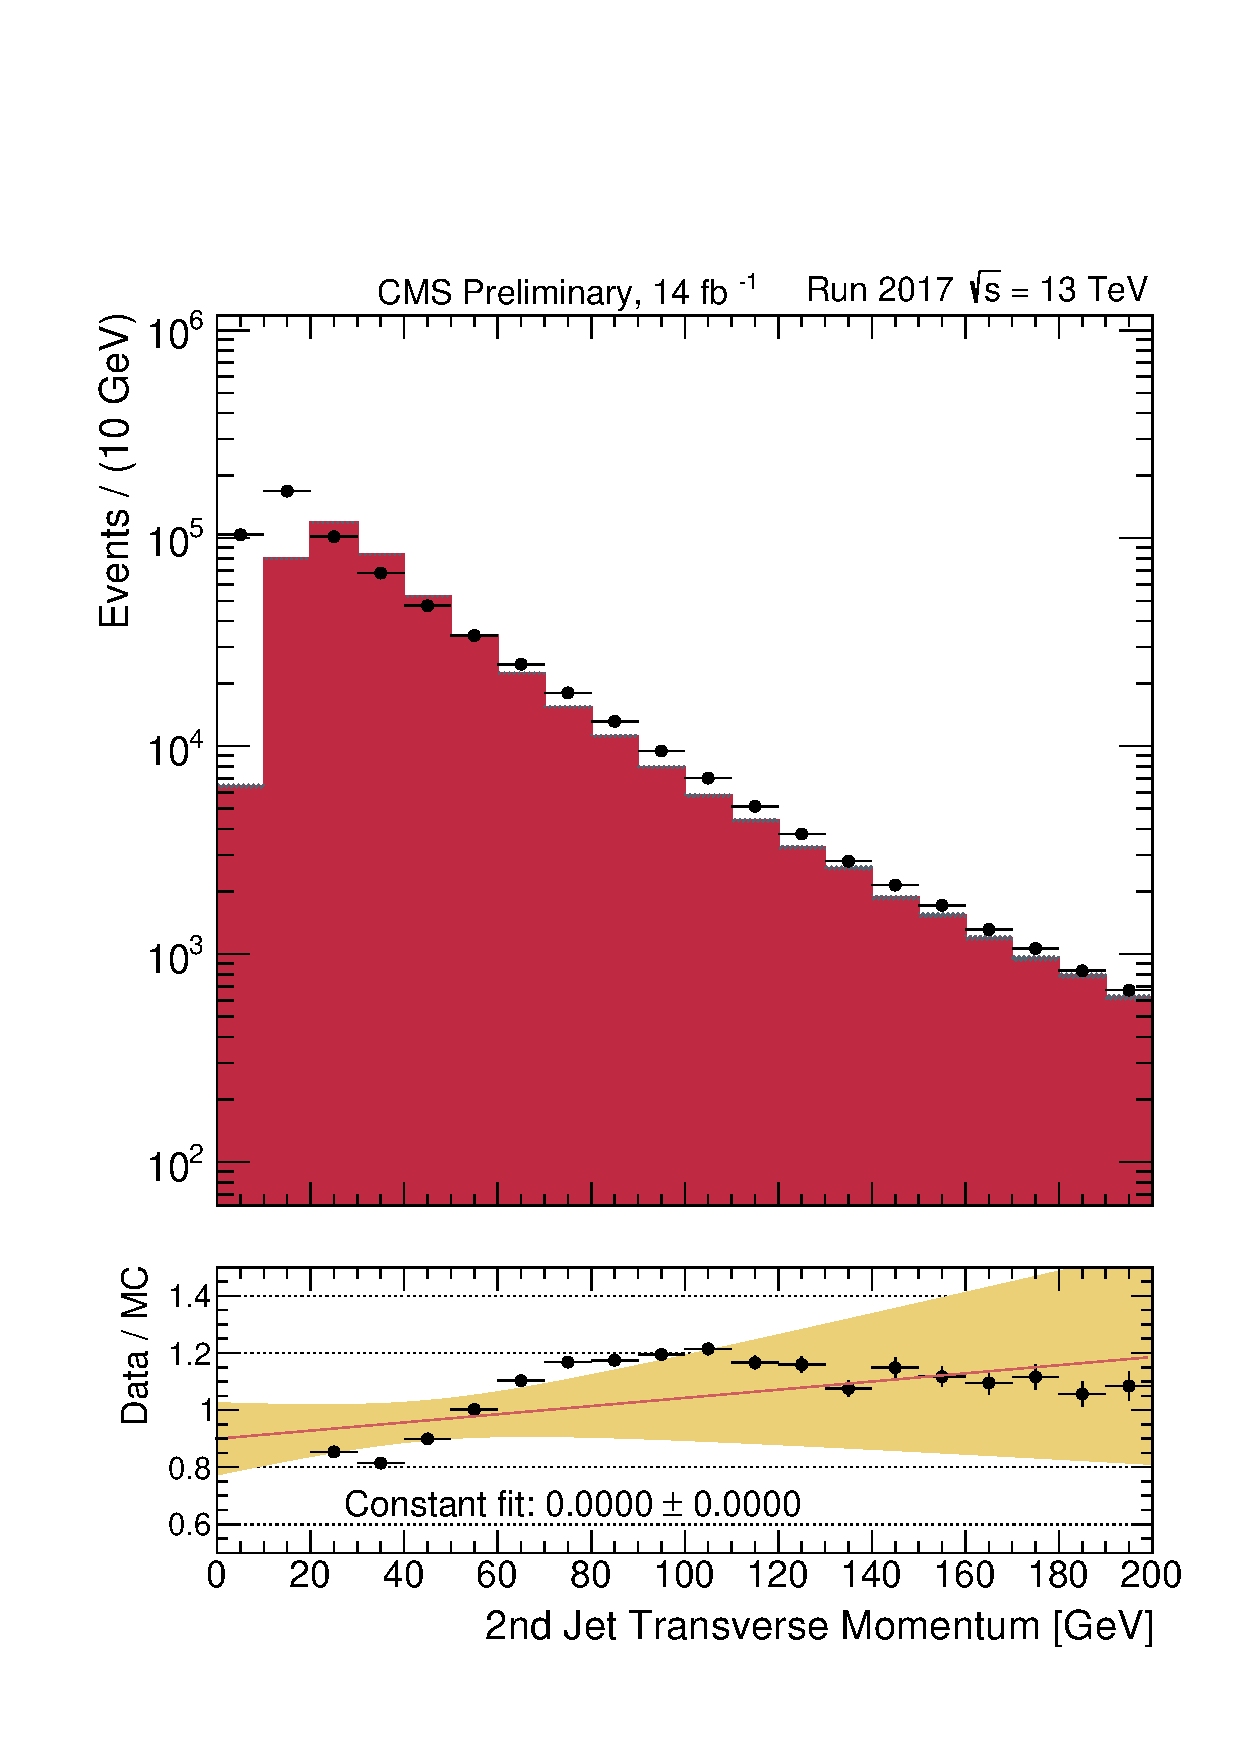
\includegraphics[width=.45\textwidth]{\PhDthesisdir/plots_and_images/my_plots/JERC/distributions/2018/with_header/ptSecondJet_log.tex}}

\caption[Observables d'événements \Gjets\ en 2018.]{Distributions d'observables dans les données (points noirs) et les simulations (histogramme en rouge) pour l'année 2018. Sur la figure~\ref{subfig-distrib_Gjets_18_ptPhoton}, l'effet des \emph{prescales} (voir page~\pageref{tab-HLT_pT_precales_18_and_17UL}) donnant une distribution en dents de scie est clairement visible.}
\label{fig-distribs_Gjets_18}
\end{figure}
\paragraph{Activité additionnelle des jets supplémentaires}
La présence d'un jet secondaire, comme sur la figure~\ref{subfig-Gamma_plus_two_jets}, créé un déséquilibre dans \Rbal\ dû à la physique de l'événement et non à la JES. Il ne faut donc pas corriger cet effet.
Pour cela, il faut pouvoir se ramener au cas où un seul jet est présent, comme dans l'événement de la figure~\ref{subfig-Gamma_plus_jet_basic_event}.
L'activité additionnelle liée aux jets supplémentaires est quantifiée par la variable
\begin{equation}
\alpha = \frac{\pT_\reco^\text{jet 2}}{\pT^{\photon}}
\mend
\label{eq-chapter-JERC-definition_alpha}
\end{equation}
\par L'analyse des événements \Gjets\ est alors réalisée pour différents intervalles de $\alpha$ afin de pouvoir réaliser par la suite une extrapolation à $\alpha=0$, correspondant au cas idéal d'événements \Gjet.
Les intervalles utilisés sont présentés dans le tableau~\ref{tab-alpha_intervalles}.
Il s'agit d'intervalles inclusifs, \ie\ que chaque intervalle contient l'intervalle précédent.
L'évolution des réponses moyennes en fonction de $\alpha$ y étant linéaire \aposteriori, ce qui se retrouve dans les résultats de la figure~\ref{fig-chapter-JERC-section-JES-subsec-analyse-responsebal_and_MPF_eta0013_ptPhot_175_230_extrap}, page~\pageref{fig-chapter-JERC-section-JES-subsec-analyse-responsebal_and_MPF_eta0013_ptPhot_175_230_extrap}, ce choix rend possible une extrapolation simple vers $\alpha=0$.
\begin{table}[h]
\centering
\begin{tabular}{ccccc}
\toprule
$[\num{0}\isp \num{0.10}[$ & $[\num{0}\isp \num{0.15}[$ & $[\num{0}\isp \num{0.20}[$ & $[\num{0}\isp \num{0.25}[$ & $[\num{0}\isp \num{0.30}[$ \\
\bottomrule
\end{tabular}
\caption{Intervalles de $\alpha$ utilisés pour la JES.}
\label{tab-alpha_intervalles}
\end{table}
\par Des études sont en cours afin d'inclure des valeurs de $\alpha$ allant jusqu'à \num{1}.
L'exploitation des événements tels que $\alpha>\num{0.3}$ est doublement motivée.
Ces événements permettraient d'améliorer les corrections vis-à-vis du FSR introduit page~\pageref{subfig-fgraph-gq_qGamma_S-FSR_2jets} et les corrections à bas \pT.
En effet, pour $\pT^{\photon}<\SI{100}{\GeV}$, imposer $\alpha<\num{0.3}$ implique $\pT^\text{jet 2}<\SI{30}{\GeV}$, ce qui limite fortement le nombre d'événements exploitables.
%Mikko:
%The alpha>0.3 values are not (yet) used to constrain the FSR correction because they are outside the linear regime, but I’m working on including them for better low pT constraints. It’s a new unexplored region so taking some time to understand to sufficient detail.
%The alpha values higher than 0.3 may be necessary for reliably extending the measurement below pT<100 GeV. Here alpha<0.3 corresponds to pT2=30 GeV, which is the threshold below which pileup jet rates start to rapidly increase. This leads to large alpha cut inefficiencies and strong bias on average <rho> (i.e. PU profile). So the best solution might be to have a sliding cut of alpha<30 GeV/pT,gamma at pT<100 GeV instead of fixed 0.3.
%On the other hand, I know that dR/dalpha is quite linear at alpha<0.3 so initially I was thinking that having steps of fixed values of alpha could work, where alphamax > 30 GeV/pTZ. There are topological boundaries like ~0.35, where the second jet is almost the same pT as leading jet, if both opposite to Z. For values alpha>0.5 the second jet usually has to be opposite to the leading jet and on the same side as Z (as DeltaPhi forces it to be either parallel or antiparallel, unless it’s a three jet event). This make dR/dalpha flatten out at ~0.35-0.5 and then change sign at alpha>0.5.
%So from the initial Z+jet studies in Helsinki it seems like thresholds of alpha<0.5 (safe down to pT=60 GeV) and alpha<1.0 (safe down to pT=30 GeV) could be quite useful for low pT. The MPF method in particular is still robust for these values, and we actually have <pT1>/<pTZ> close to unity than for alpha<0.3, which has essentially maximised the difference in <pT1> and <pTZ>.
%I’ve not yet activated alpha<0.5 and 1.0 because they are missing from the official Z+jet inputs from KIT (I only have them in our Helsinki study, which is in other respects less advanced than the KIT one). I also foresee needing the unclustered energy and secondary jet sum estimates for properly correcting MPF without extrapolated FSR correction in the non-linear regime.
\paragraph{Obtention des corrections pour $\pT^{\photon}, \eta^\text{jet}, (\alpha^\text{max})$ donnés}
Pour chaque domaine
de $\pT^{\photon}$ défini dans le tableau~\ref{tab-pT_photon_intervalles},
de $\eta^\text{jet}$ défini dans le tableau~\ref{tab-eta_jet_intervalles_large} et
de $\alpha$ défini dans le tableau~\ref{tab-alpha_intervalles},
les distributions des réponses balancée et MPF des données et des simulations sont déterminées.
Certaines de ces distributions sont représentées sur la figure~\ref{fig-distribs_Gjets_18_resp_bal_and_mpf}.
\par Afin de limiter les effets des queues de ces distributions, en particulier dans le cas de la réponse balancée,
une troncature leur est appliquée pour n'en conserver que les parties centrales.
Pour cela, un ajustement à une gaussienne est réalisé pour chaque distribution.
Les points considérés dans la suite sont alors ceux appartenant à un intervalle  $[ \bar{R} - \Delta R, \bar{R} + \Delta R ]$ où $\bar{R}$ est le centre de la gaussienne obtenue et $\Delta R$ est fixé tel que l'intégrale de la distribution tronquée représente \SI{98.5}{\%} de l'intégrale de la distribution initiale.
Une estimation des moyennes de ces distributions tronquées est alors obtenue ; ces moyennes sont représentées sur la figure~\ref{fig-distribs_Gjets_18_resp_bal_and_mpf}.
Un écart est effectivement observé entre données et simulations.
Il s'agit précisément de l'écart que la correction résiduelle absolue en \pT\ des jets doit corriger.
\begin{figure}[h]
\centering
\subcaptionbox{Réponse balancée pour $\pT^{\photon}\in[175, 230[$ \SI{}{\GeV}.\label{subfig-distrib_Gjets_18_resp_balancing_eta0013_ptPhot_175_230}}[.45\textwidth]
{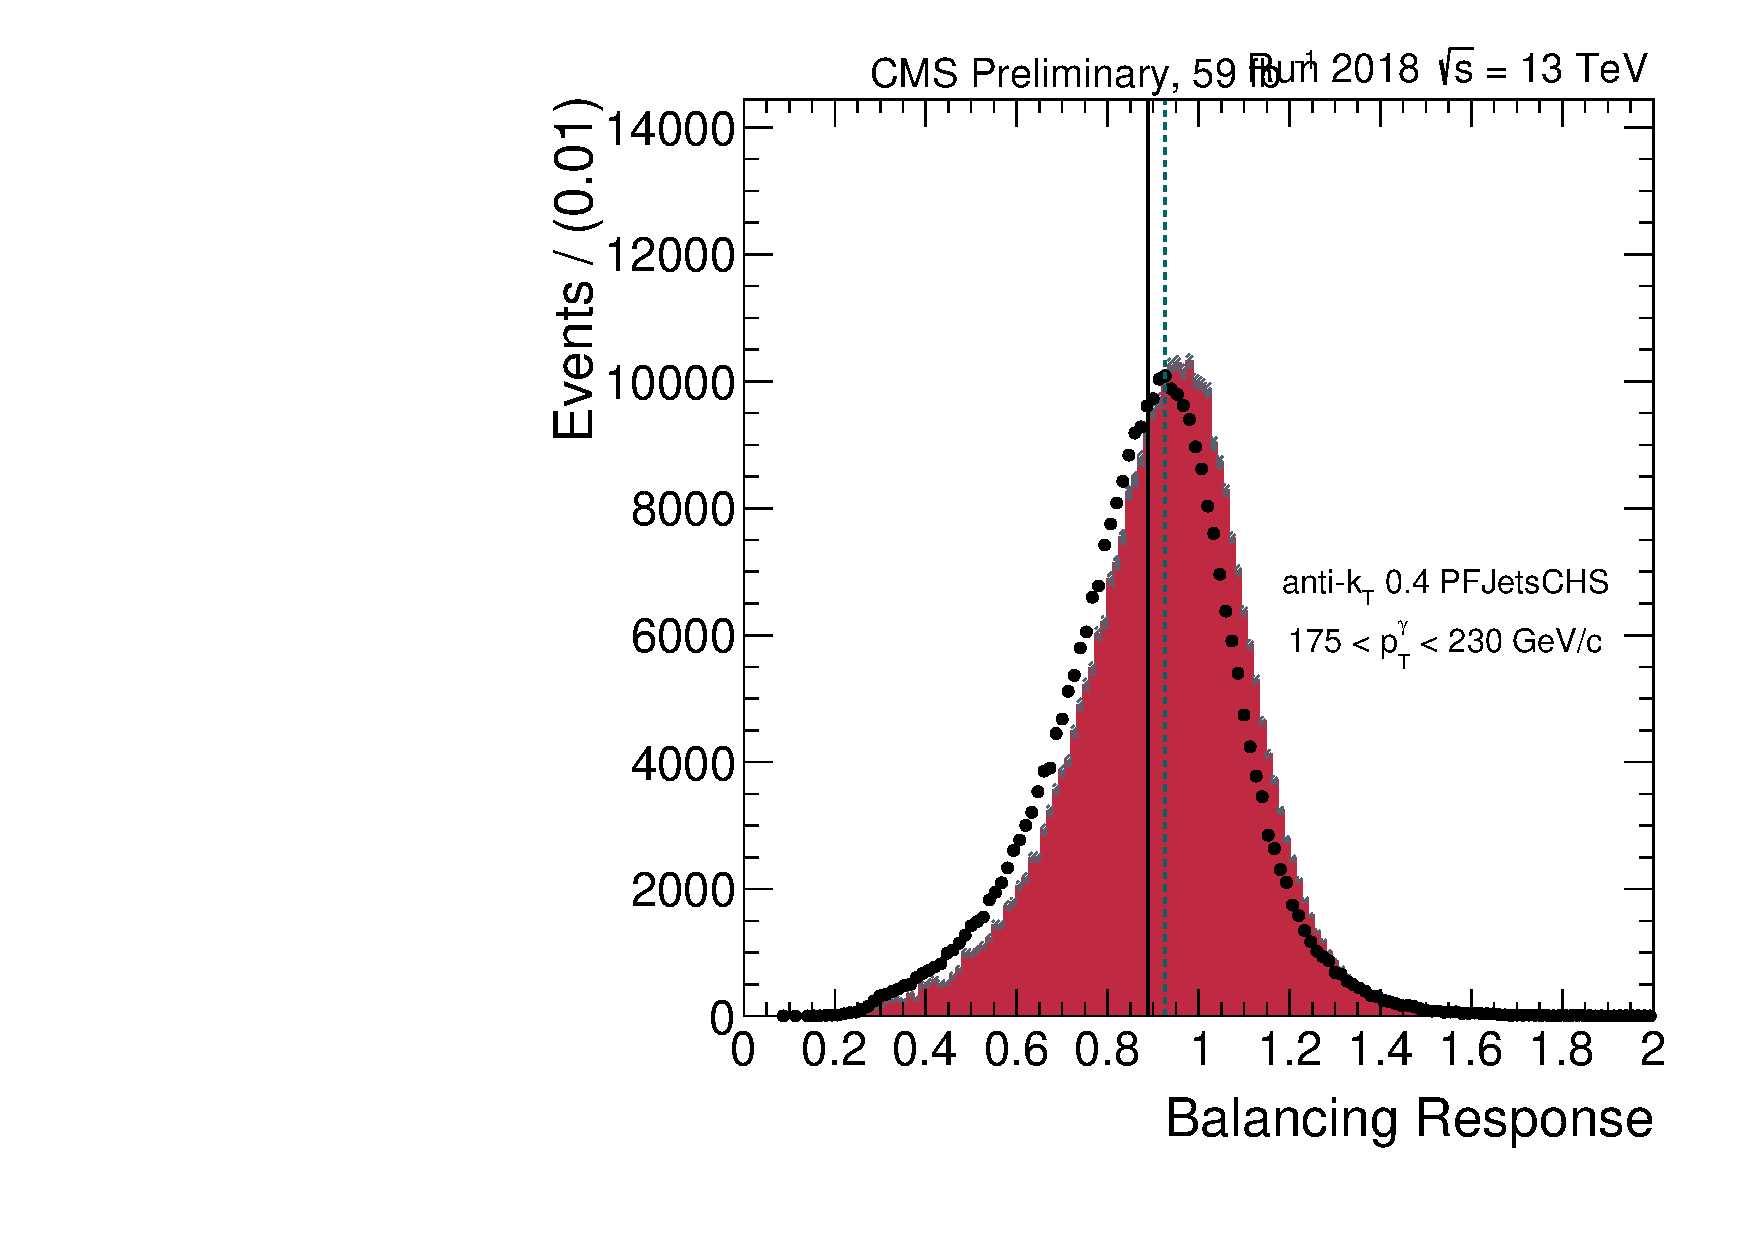
\includegraphics[width=.45\textwidth]{\PhDthesisdir/plots_and_images/my_plots/JERC/distributions/2018/with_header/resp_balancing_eta0013_ptPhot_175_230.tex}}
\hfill
\subcaptionbox{Réponse balancée pour $\pT^{\photon}\in[300, 400[$ \SI{}{\GeV}.\label{subfig-distrib_Gjets_18_resp_balancing_eta0013_ptPhot_300_400}}[.45\textwidth]
{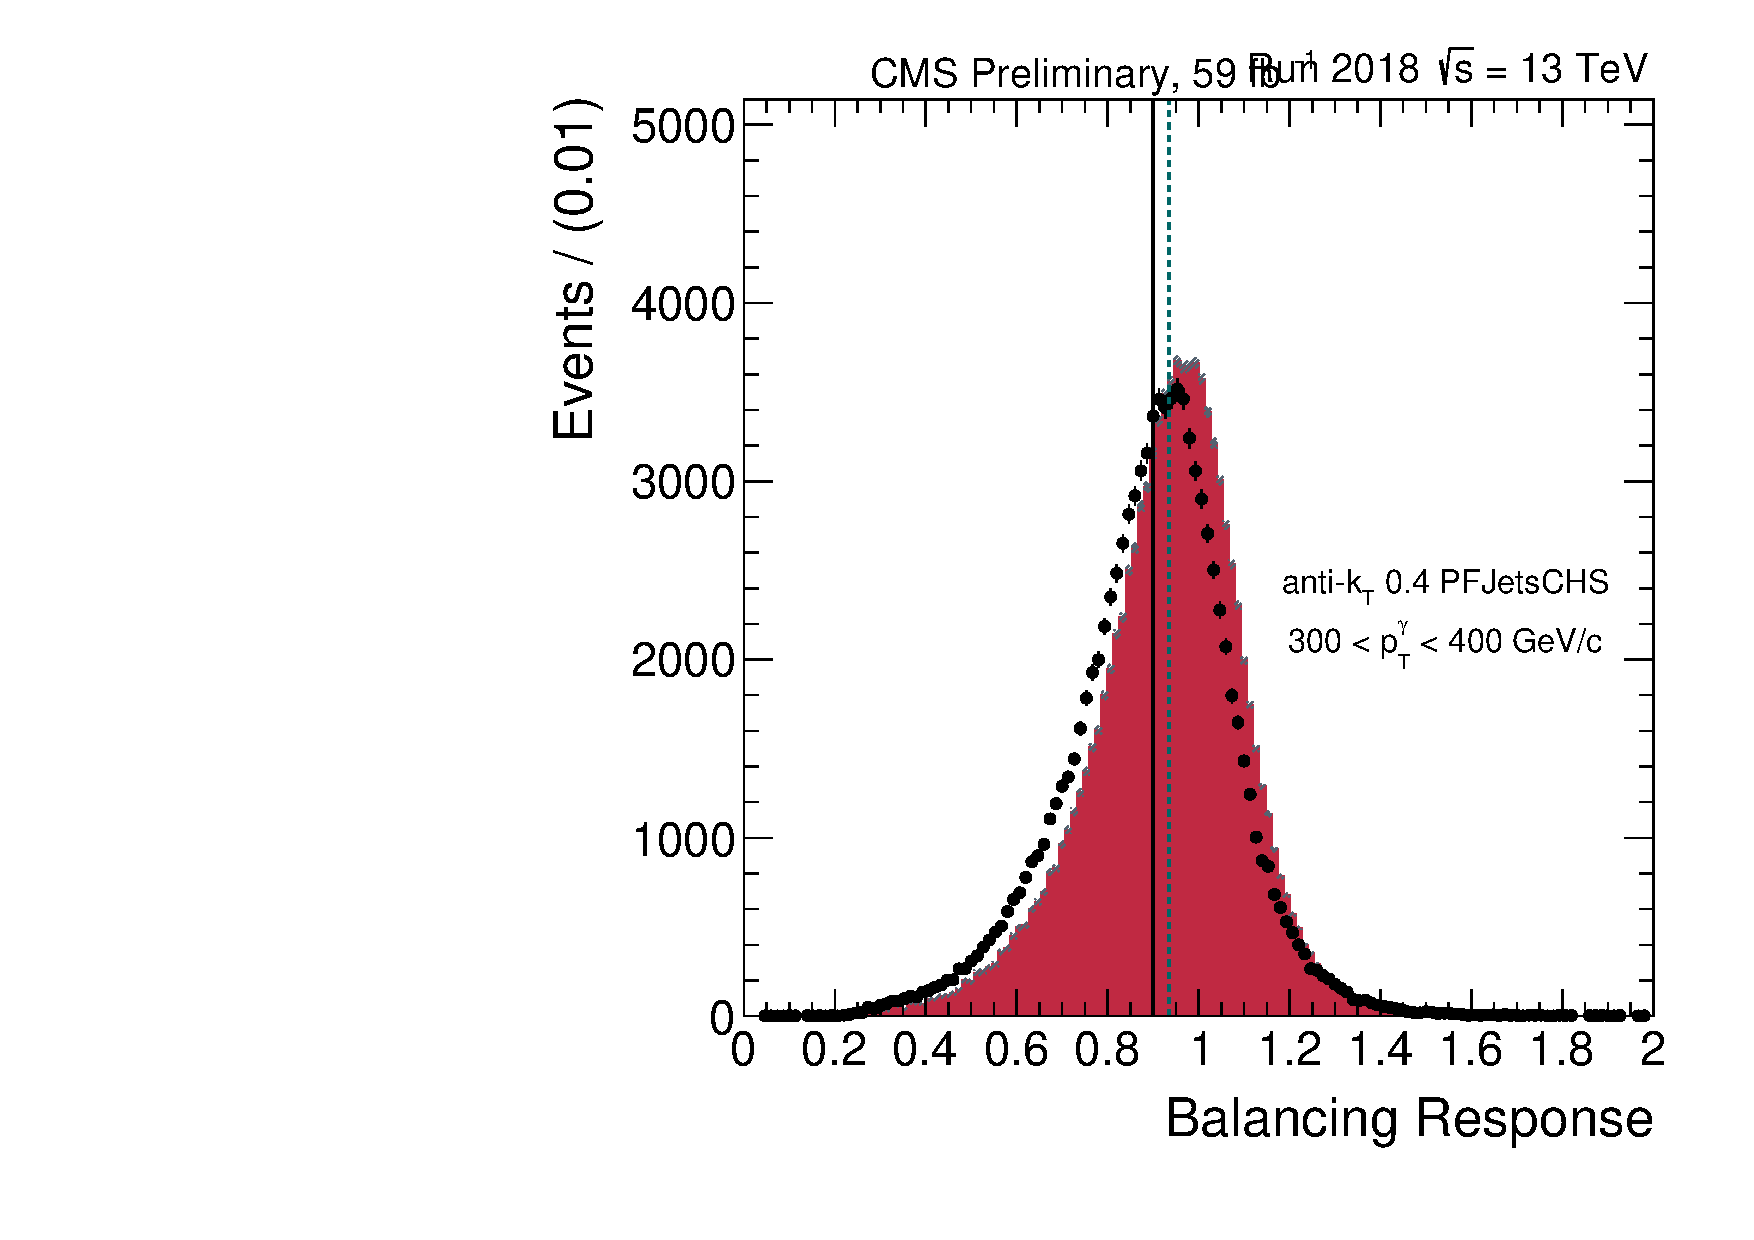
\includegraphics[width=.45\textwidth]{\PhDthesisdir/plots_and_images/my_plots/JERC/distributions/2018/with_header/resp_balancing_eta0013_ptPhot_300_400.tex}}

\vspace{.5\baselineskip}

\subcaptionbox{Réponse MPF pour $\pT^{\photon}\in[175, 230[$ \SI{}{\GeV}.\label{subfig-distrib_Gjets_18_resp_mpf_eta0013_ptPhot_175_230}}[.45\textwidth]
{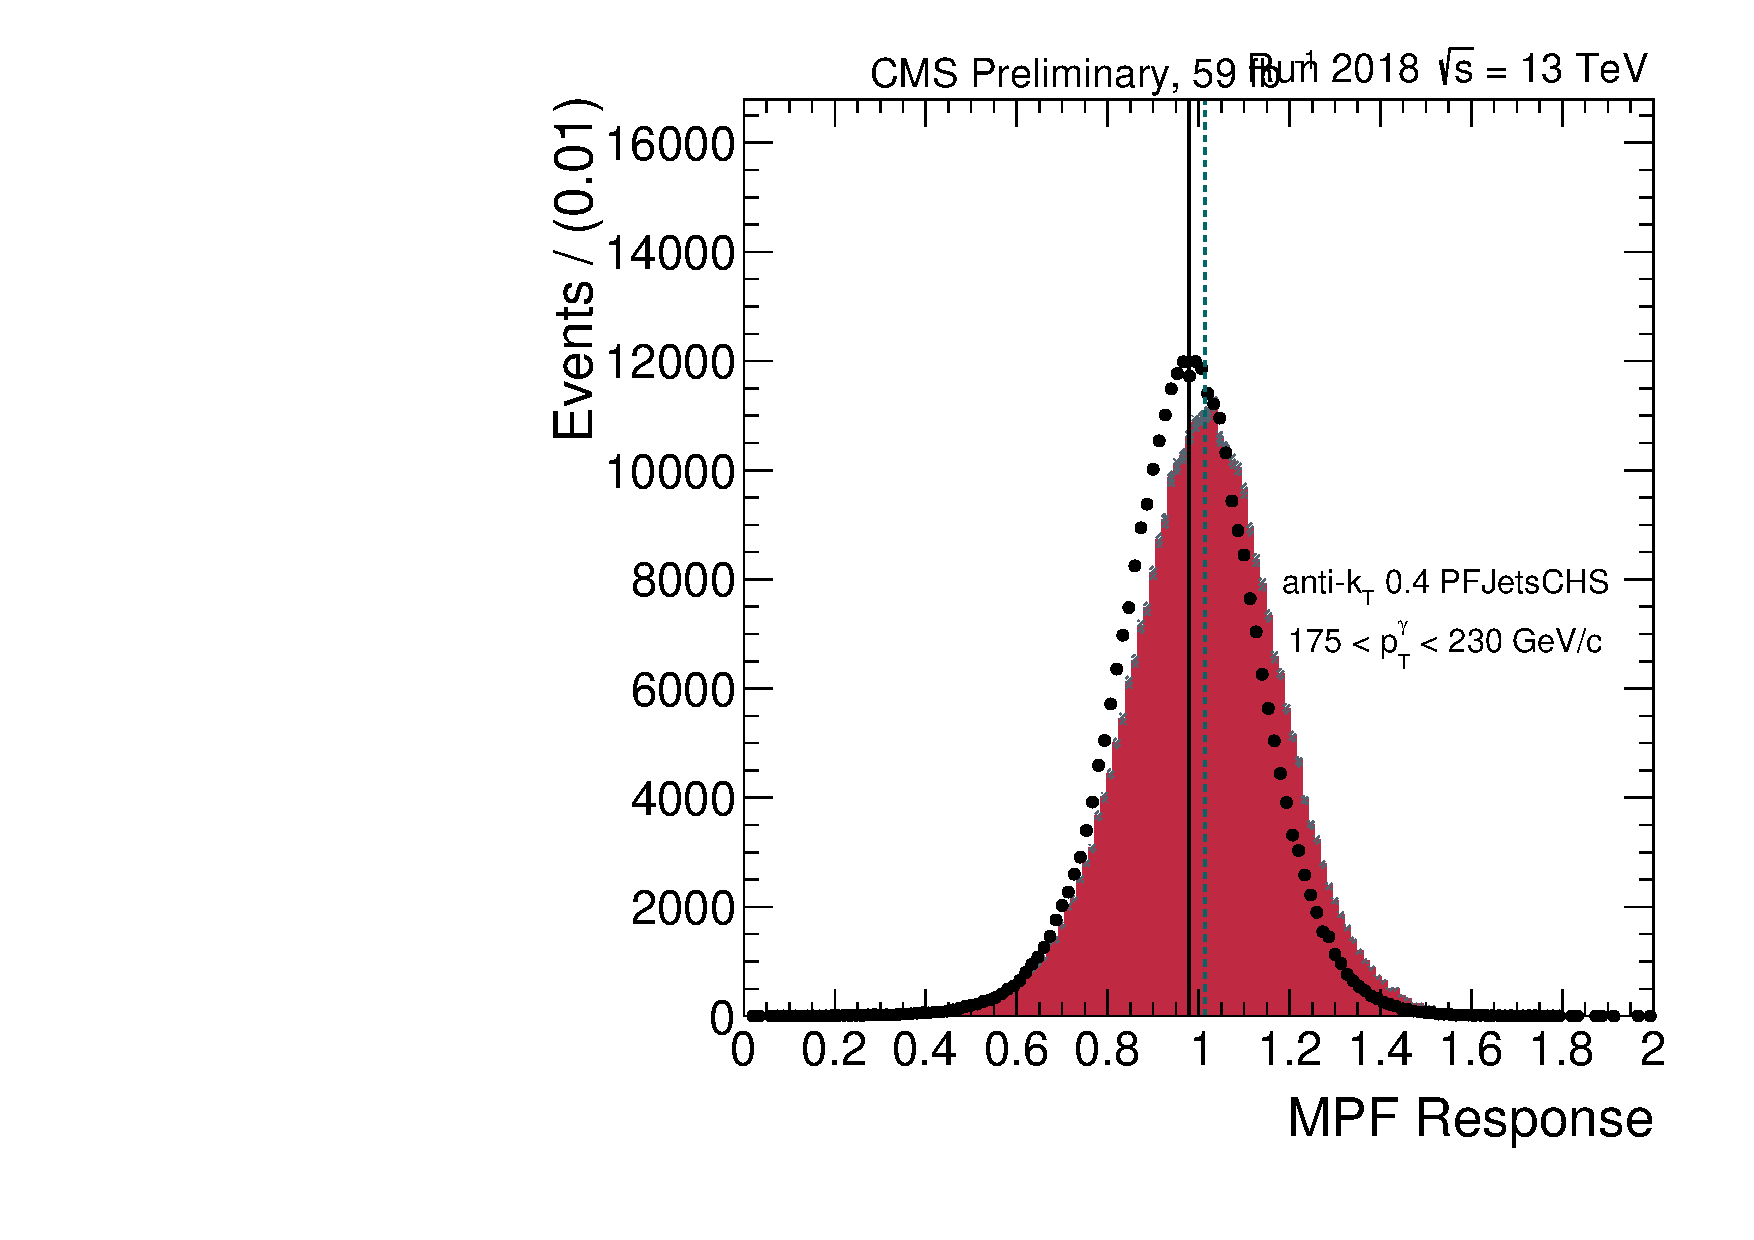
\includegraphics[width=.45\textwidth]{\PhDthesisdir/plots_and_images/my_plots/JERC/distributions/2018/with_header/resp_mpf_eta0013_ptPhot_175_230.tex}}
\hfill
\subcaptionbox{Réponse MPF pour $\pT^{\photon}\in[300, 400[$ \SI{}{\GeV}.\label{subfig-distrib_Gjets_18_resp_mpf_eta0013_ptPhot_300_400}}[.45\textwidth]
{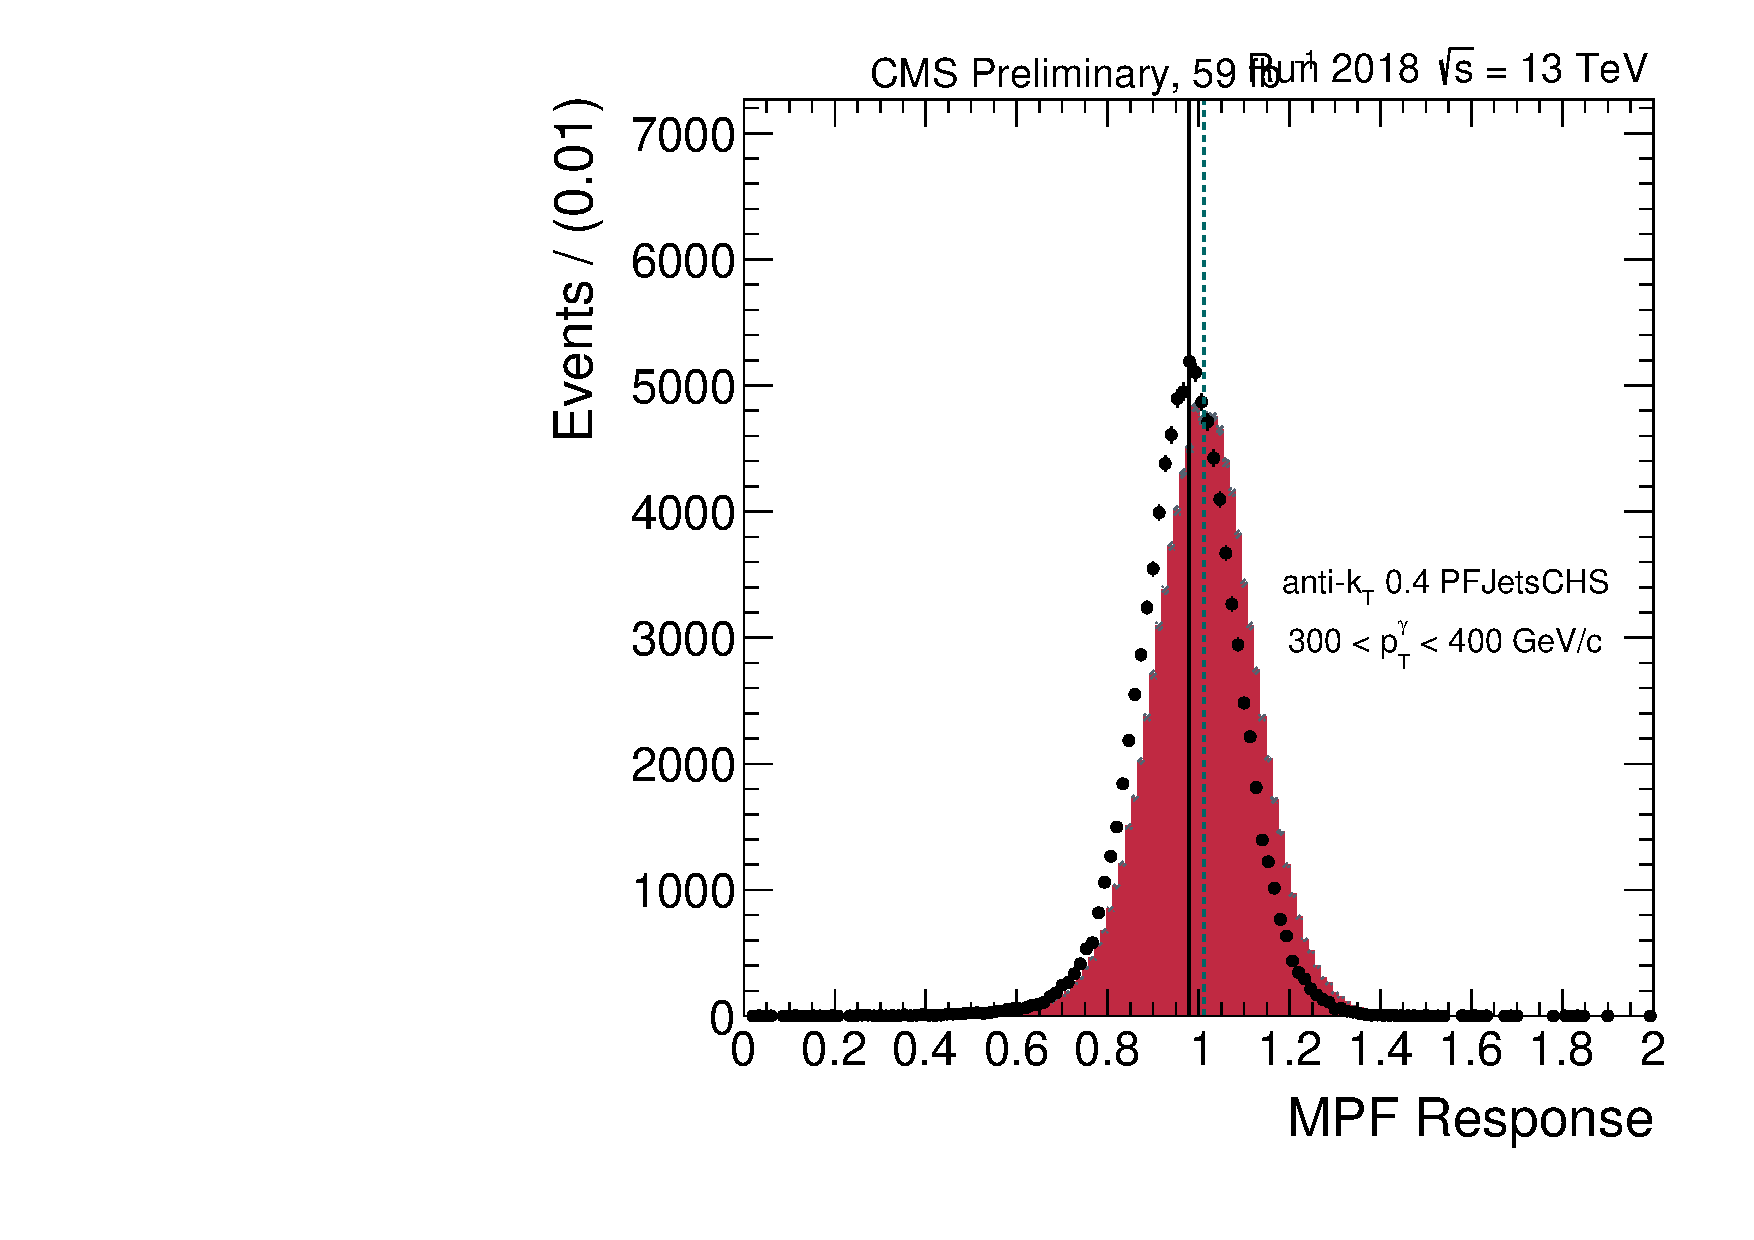
\includegraphics[width=.45\textwidth]{\PhDthesisdir/plots_and_images/my_plots/JERC/distributions/2018/with_header/resp_mpf_eta0013_ptPhot_300_400.tex}}

\caption[Réponses balancée et MPF en 2018.]{Réponses balancée et MPF dans les données (points noirs) et simulations (histogramme en rouge) pour $\alpha<\num{0.3}$, $\abs{\eta^\text{jet}}<\num{1.3}$ et deux intervalles de $\pT^{\photon}$ en 2018.}
\label{fig-distribs_Gjets_18_resp_bal_and_mpf}
\end{figure}
\paragraph{Extrapolation vers $\alpha=0$}
Une extrapolation vers $\alpha=0$ est réalisée afin de s'affranchir de l'activité additionnelle des jets décrite dans la section~\ref{chapter-JERC-section-pheno-GJets-subsec-effets_radiatifs}.
Les intervalles de $\alpha$ utilisés pour la JES sont présentés dans le tableau~\ref{tab-alpha_intervalles}.
L'utilisation des ces intervalles inclusifs permet une extrapolation linéaire en $\alpha$, ce qui est réalisé sur la figure~\ref{fig-chapter-JERC-section-JES-subsec-analyse-responsebal_and_MPF_eta0013_ptPhot_175_230_extrap}.
\begin{figure}[h]
\centering
\subcaptionbox{Réponse balancée.\label{subfig-chapter-JERC-section-JES-subsec-analyse-response_eta0013_ptPhot_175_230_extrap}}[.45\textwidth]
{\includegraphics[width=.45\textwidth]{\PhDthesisdir/plots_and_images/my_plots/JERC/only_L2Res/Run2018ABCD/extrapolation/response_eta0013_ptPhot_175_230.tex}}
\hfill
\subcaptionbox{Réponse MPF.\label{subfig-chapter-JERC-section-JES-subsec-analyse-responseMPF_eta0013_ptPhot_175_230_extrap}}[.45\textwidth]
{\includegraphics[width=.45\textwidth]{\PhDthesisdir/plots_and_images/my_plots/JERC/only_L2Res/Run2018ABCD/extrapolation/responseMPF_eta0013_ptPhot_175_230.tex}}
\caption[Extrapolation vers $\alpha=0$ de la réponse des jets.]{Extrapolation vers $\alpha=0$ de la réponse des jets pour $\abs{\eta}<\num{1.3}$ et $\num{175}<\pT^{\photon}<\SI{230}{\GeV}$ en 2018.}
\label{fig-chapter-JERC-section-JES-subsec-analyse-responsebal_and_MPF_eta0013_ptPhot_175_230_extrap}
\end{figure}
\subsection{Résultats}\label{chapter-JERC-section-JES-subsec-results}
La correction à appliquer aux données, définie par la formule~\eqref{eq-chapter-JERC-section-CMS-subsec-residuals-Cres_def} d'après la démarche exposée dans la section~\ref{chapter-JERC-section-CMS-subsec-residuals}, s'obtient en calculant la valeur moyenne des réponses \Rbal\ ou \RMPF\ pour les données et les simulations dans chacun des intervalles
de $\pT^{\photon}$ défini dans le tableau~\ref{tab-pT_photon_intervalles} et
de $\eta^\text{jet}$ défini dans le tableau~\ref{tab-eta_jet_intervalles_large}.
Elle permet de ramener la réponse moyenne des jets dans les données à celle constatée dans les simulations.
\par Les résultats ainsi obtenus à l'aide des méthodes de la balance et MPF, avant et après extrapolation vers $\alpha=0$, sont présentés dans les sections~\ref{chapter-JERC-section-JES-subsec-results-subsubsec-before_extrap} et~\ref{chapter-JERC-section-JES-subsec-results-subsubsec-after_extrap}.
Les distributions moyennes des réponses en fonction de $\pT^{\photon}$ dans les données et les simulations, ainsi que leurs rapports, y sont représentés.
Un ajustement constant est réalisé dans chaque intervalle de $\eta^\text{jet}$ afin d'obtenir un ordre de grandeur de la correction à appliquer dans cet intervalle.
La dépendance en $\pT$ de la correction est déterminée grâce à un ajustement global réalisé avec les résultats d'autres analyses, présenté dans la section~\ref{chapter-JERC-section-JES-subsec-results-subsubsec-global_fit}.
Enfin, une vérification de la bonne mise en œuvre de la correction ainsi déterminée est présentée dans la section~\ref{chapter-JERC-section-JES-subsec-results-subsubsec-L2L3Res_cross_check}.
\subsubsection{Résultats avant extrapolation}\label{chapter-JERC-section-JES-subsec-results-subsubsec-before_extrap}
\par Les distributions des réponses balancées avant extrapolation se trouvent figure~\ref{fig-responses_balancing_alpha_0_3_2018ABCD}, page~\pageref{fig-responses_balancing_alpha_0_3_2018ABCD}.
Les corrections à appliquer sont de l'ordre
de \SI{4}{\%} pour $\abs{\eta^\text{jet}} < \num{1.3}$,
de \SI{6}{\%} pour $\num{1.3} \leq \abs{\eta^\text{jet}} < \num{2.5}$ et
de \SI{3}{\%} pour $\abs{\eta^\text{jet}} > \num{2.5}$.
\par Les distributions des réponses MPF avant extrapolation se trouvent figure~\ref{fig-responses_MPF_alpha_0_3_2018ABCD}, page~\pageref{fig-responses_MPF_alpha_0_3_2018ABCD}.
Les corrections à appliquer sont de l'ordre
de \SI{3}{\%} pour $\abs{\eta^\text{jet}} < \num{1.3}$,
de \SI{5}{\%} pour $\num{1.3} \leq \abs{\eta^\text{jet}} < \num{2.5}$, soit environ \SI{1}{\%} de moins qu'avec la méthode balancée, et
de \SI{3}{\%} pour $\abs{\eta^\text{jet}} > \num{2.5}$,
\par Il est à noter que ces résultats sont obtenus avant extrapolation vers $\alpha=0$. Or, cette extrapolation a un effet beaucoup plus important sur la réponse balancée que sur la réponse MPF, comme le montre la figure~\ref{fig-chapter-JERC-section-JES-subsec-analyse-responsebal_and_MPF_eta0013_ptPhot_175_230_extrap}.
\subsubsection{Résultats après extrapolation}\label{chapter-JERC-section-JES-subsec-results-subsubsec-after_extrap}
L'extrapolation des réponses vers $\alpha=0$ est réalisée comme expliqué dans la section~\ref{chapter-JERC-section-JES-subsec-analyse}.
\par Les distributions des réponses balancées après extrapolation se trouvent figure~\ref{fig-responses_balancing_extrapolated_2018ABCD}, page~\pageref{fig-responses_balancing_extrapolated_2018ABCD}.
Les corrections à appliquer sont de l'ordre
de \SI{3}{\%} pour $\abs{\eta^\text{jet}} < \num{1.3}$,
de \SI{5}{\%} pour $\num{1.3} \leq \abs{\eta^\text{jet}} < \num{2.5}$, soit environ \SI{1}{\%} de moins qu'avant extrapolation, et
de \SI{3}{\%} pour $\abs{\eta^\text{jet}} > \num{2.5}$.
\par Les distributions des réponses MPF après extrapolation se trouvent figure~\ref{fig-responses_MPF_extrapolated_2018ABCD}, page~\pageref{fig-responses_MPF_extrapolated_2018ABCD}.
Les corrections à appliquer sont de l'ordre
de \SI{3}{\%} pour $\abs{\eta^\text{jet}} < \num{1.3}$,
de \SI{5}{\%} pour $\num{1.3} \leq \abs{\eta^\text{jet}} < \num{2.5}$ et
de \SI{3}{\%} pour $\abs{\eta^\text{jet}} > \num{2.5}$,
soit du même ordre qu'avant extrapolation.
L'extrapolation a donc bien un effet très faible sur \RMPF.
\par Les valeurs des rapports données sur simulations des réponses balancée et MPF obtenus sont résumés dans le tableau~\ref{tab-responses_recap_table_2018ABCD}.
L'extrapolation vers $\alpha=0$ permet de rétablir l'accord entre les rapport des réponses balancée et MPF.
Cet accord permet de valider l'utilisation de ces méthodes afin d'estimer la JES.

\begin{table}[h]
\centering
\begin{tabular}{lcccc}
\toprule
\multirow{2}{*}{$\abs{\eta^\text{jet}}\in$} & \multicolumn{2}{c}{Réponse balancée} & \multicolumn{2}{c}{Réponse MPF} \\
\cmidrule(lr){2-3}\cmidrule(lr){4-5}
 & $\alpha<\num{0.3}$ & $\alpha\to0$ & $\alpha<\num{0.3}$ & $\alpha\to0$\\
\midrule
$[\num{0}\isp \num{1.3}[$ & $\num{0.9581}\pm\num{0.0003}$ & $\num{0.9669}\pm\num{0.0004}$ & $\num{0.9667}\pm\num{0.0002}$ & $\num{0.9687}\pm\num{0.0003}$ \\
$[\num{1.3}\isp \num{2.0}[$ & $\num{0.9426}\pm\num{0.0006}$ & $\num{0.9538}\pm\num{0.0009}$ & $\num{0.9521}\pm\num{0.0004}$ & $\num{0.9565}\pm\num{0.0008}$ \\
$[\num{2.0}\isp \num{2.5}[$ & $\num{0.9425}\pm\num{0.0010}$ & $\num{0.9502}\pm\num{0.0015}$ & $\num{0.9508}\pm\num{0.0007}$ & $\num{0.9516}\pm\num{0.0014}$ \\
$[\num{2.5}\isp \num{3.0}[$ & $\num{0.9744}\pm\num{0.0026}$ & $\num{0.9661}\pm\num{0.0037}$ & $\num{0.9689}\pm\num{0.0018}$ & $\num{0.9707}\pm\num{0.0034}$ \\
\bottomrule
\end{tabular}
\caption[Rapports des réponses balancée et MPF obtenus en 2018.]{Rapports données réelles sur simulées des réponses balancée et MPF obtenus en 2018.}
\label{tab-responses_recap_table_2018ABCD}
\end{table}

\begin{figure}[p]
\centering
\subcaptionbox{$\abs{\eta^\text{jet}} < \num{1.3}$.\label{subfig-response_eta0013_balancing_alpha_0_3_2018ABCD}}[.45\textwidth]
{\includegraphics[width=.45\textwidth]{\PhDthesisdir/plots_and_images/my_plots/JERC/only_L2Res/Run2018ABCD/alpha_0_3/response_eta0013_balancing.pdf}}
\hfill
\subcaptionbox{$\num{1.3} \leq \abs{\eta^\text{jet}} < \num{2.0}$.\label{subfig-response_eta1319_balancing_alpha_0_3_2018ABCD}}[.45\textwidth]
{\includegraphics[width=.45\textwidth]{\PhDthesisdir/plots_and_images/my_plots/JERC/only_L2Res/Run2018ABCD/alpha_0_3/response_eta1319_balancing.pdf}}

\vfill

\subcaptionbox{$\num{2.0} \leq \abs{\eta^\text{jet}} < \num{2.5}$.\label{subfig-response_eta1925_balancing_alpha_0_3_2018ABCD}}[.45\textwidth]
{\includegraphics[width=.45\textwidth]{\PhDthesisdir/plots_and_images/my_plots/JERC/only_L2Res/Run2018ABCD/alpha_0_3/response_eta1925_balancing.pdf}}
\hfill
\subcaptionbox{$\num{2.5} \leq \abs{\eta^\text{jet}} < \num{3.0}$.\label{subfig-response_eta2530_balancing_alpha_0_3_2018ABCD}}[.45\textwidth]
{\includegraphics[width=.45\textwidth]{\PhDthesisdir/plots_and_images/my_plots/JERC/only_L2Res/Run2018ABCD/alpha_0_3/response_eta2530_balancing.pdf}}

\caption[Réponses balancées en 2018 avant extrapolation.]{Distributions des réponses balancées moyennes en fonction de $\pT^{\text{\photon}}$ pour différents intervalles de $\eta^\text{jet}$ en 2018 avant extrapolation. Le rapport données sur simulations est présenté dans chaque cas ainsi qu'un ajustement à une constante donnant l'ordre de grandeur de la correction résiduelle à appliquer.}
\label{fig-responses_balancing_alpha_0_3_2018ABCD}
\end{figure}
\begin{figure}[p]
\centering
\subcaptionbox{$\abs{\eta^\text{jet}} < \num{1.3}$.\label{subfig-response_eta0013_MPF_alpha_0_3_2018ABCD}}[.45\textwidth]
{\includegraphics[width=.45\textwidth]{\PhDthesisdir/contents/chapter-JERC/plots/my_plots/only_L2Res/Run2018ABCD/alpha_0_3/response_eta0013_mpf.pdf}}
\hfill
\subcaptionbox{$\num{1.3} \leq \abs{\eta^\text{jet}} < \num{2.0}$.\label{subfig-response_eta1319_MPF_alpha_0_3_2018ABCD}}[.45\textwidth]
{\includegraphics[width=.45\textwidth]{\PhDthesisdir/contents/chapter-JERC/plots/my_plots/only_L2Res/Run2018ABCD/alpha_0_3/response_eta1319_mpf.pdf}}

\vfill

\subcaptionbox{$\num{2.0} \leq \abs{\eta^\text{jet}} < \num{2.5}$.\label{subfig-response_eta1925_MPF_alpha_0_3_2018ABCD}}[.45\textwidth]
{\includegraphics[width=.45\textwidth]{\PhDthesisdir/contents/chapter-JERC/plots/my_plots/only_L2Res/Run2018ABCD/alpha_0_3/response_eta1925_mpf.pdf}}
\hfill
\subcaptionbox{$\num{2.5} \leq \abs{\eta^\text{jet}} < \num{3.0}$.\label{subfig-response_eta2530_MPF_alpha_0_3_2018ABCD}}[.45\textwidth]
{\includegraphics[width=.45\textwidth]{\PhDthesisdir/contents/chapter-JERC/plots/my_plots/only_L2Res/Run2018ABCD/alpha_0_3/response_eta2530_mpf.pdf}}

\caption[Réponses MPF en 2018 avant extrapolation.]{Distributions des réponses MPF moyennes en fonction de $\pT^{\text{\photon}}$ pour différents intervalles de $\eta^\text{jet}$ en 2018 avant extrapolation. Le rapport données sur simulations est présenté dans chaque cas ainsi qu'un ajustement à une constante donnant l'ordre de grandeur de la correction résiduelle à appliquer.}
\label{fig-responses_MPF_alpha_0_3_2018ABCD}
\end{figure}
\begin{figure}[p]
\centering
\subcaptionbox{$\abs{\eta^\text{jet}} < \num{1.3}$.\label{subfig-response_eta0013_balancing_extrapolated_2018ABCD}}[.45\textwidth]
{\includegraphics[width=.45\textwidth]{\PhDthesisdir/plots_and_images/my_plots/JERC/only_L2Res/Run2018ABCD/extrapolated/response_eta0013_balancing_extrap.tex}}
\hfill
\subcaptionbox{$\num{1.3} \leq \abs{\eta^\text{jet}} < \num{2.0}$.\label{subfig-response_eta1319_balancing_extrapolated_2018ABCD}}[.45\textwidth]
{\includegraphics[width=.45\textwidth]{\PhDthesisdir/plots_and_images/my_plots/JERC/only_L2Res/Run2018ABCD/extrapolated/response_eta1319_balancing_extrap.tex}}

\vfill

\subcaptionbox{$\num{2.0} \leq \abs{\eta^\text{jet}} < \num{2.5}$.\label{subfig-response_eta1925_balancing_extrapolated_2018ABCD}}[.45\textwidth]
{\includegraphics[width=.45\textwidth]{\PhDthesisdir/plots_and_images/my_plots/JERC/only_L2Res/Run2018ABCD/extrapolated/response_eta1925_balancing_extrap.tex}}
\hfill
\subcaptionbox{$\num{2.5} \leq \abs{\eta^\text{jet}} < \num{3.0}$.\label{subfig-response_eta2530_balancing_extrapolated_2018ABCD}}[.45\textwidth]
{\includegraphics[width=.45\textwidth]{\PhDthesisdir/plots_and_images/my_plots/JERC/only_L2Res/Run2018ABCD/extrapolated/response_eta2530_balancing_extrap.tex}}

\caption[Réponses équilibrées en 2018 apr\`es extrapolation.]{Distributions des réponses équilibrées moyennes en fonction de $\pT^{\text{\photon}}$ pour différents intervalles de $\eta^\text{jet}$ en 2018 apr\`es extrapolation. Le rapport données réelles sur simulées est présenté dans chaque cas ainsi qu'un ajustement à une constante donnant l'ordre de grandeur de la correction résiduelle à appliquer.}
\label{fig-responses_balancing_extrapolated_2018ABCD}
\end{figure}
\begin{figure}[p]
\centering
\subcaptionbox{$\abs{\eta^\text{jet}} < \num{1.3}$.\label{subfig-response_eta0013_MPF_extrapolated_2018ABCD}}[.45\textwidth]
{\includegraphics[width=.45\textwidth]{\PhDthesisdir/plots_and_images/my_plots/JERC/only_L2Res/Run2018ABCD/extrapolated/response_eta0013_mpf_extrap.pdf}}
\hfill
\subcaptionbox{$\num{1.3} \leq \abs{\eta^\text{jet}} < \num{2.0}$.\label{subfig-response_eta1319_MPF_extrapolated_2018ABCD}}[.45\textwidth]
{\includegraphics[width=.45\textwidth]{\PhDthesisdir/plots_and_images/my_plots/JERC/only_L2Res/Run2018ABCD/extrapolated/response_eta1319_mpf_extrap.pdf}}

\vfill

\subcaptionbox{$\num{2.0} \leq \abs{\eta^\text{jet}} < \num{2.5}$.\label{subfig-response_eta1925_MPF_extrapolated_2018ABCD}}[.45\textwidth]
{\includegraphics[width=.45\textwidth]{\PhDthesisdir/plots_and_images/my_plots/JERC/only_L2Res/Run2018ABCD/extrapolated/response_eta1925_mpf_extrap.pdf}}
\hfill
\subcaptionbox{$\num{2.5} \leq \abs{\eta^\text{jet}} < \num{3.0}$.\label{subfig-response_eta2530_MPF_extrapolated_2018ABCD}}[.45\textwidth]
{\includegraphics[width=.45\textwidth]{\PhDthesisdir/plots_and_images/my_plots/JERC/only_L2Res/Run2018ABCD/extrapolated/response_eta2530_mpf_extrap.pdf}}

\caption[Réponses MPF en 2018 apr\`es extrapolation.]{Distributions des réponses MPF moyennes en fonction de $\pT^{\text{\photon}}$ pour différents intervalles de $\eta^\text{jet}$ en 2018 apr\`es extrapolation. Le rapport données sur simulations est présenté dans chaque cas ainsi qu'un ajustement à une constante donnant l'ordre de grandeur de la correction résiduelle à appliquer.}
\label{fig-responses_MPF_extrapolated_2018ABCD}
\end{figure}

\subsubsection{Ajustement global}\label{chapter-JERC-section-JES-subsec-results-subsubsec-global_fit}
Les événements \Gjets\ ne permettent pas à eux seuls de couvrir avec une statistique suffisante l'ensemble de la gamme d'impulsions transverses à calibrer.
De plus, l'utilisation de différentes catégories d'événements permet de valider \aposteriori\ les résultats des analyses entre elles.
Un ajustement global est alors réalisé sur les événements \Zjets, \Gjets\ et multijet afin d'obtenir la correction finale à appliquer aux données.
\par Cet ajustement est réalisé en minimisant un $\chi^2$ prenant en compte les contraintes de chaque catégorie d'événements.
La correction résiduelle absolue en \pT\ des jets correspond ainsi à l'ajustement d'une fonction paramétrique.
Les incertitudes présentes dans les différentes analyses sont considérées comme des paramètres de nuisance pour l'ajustement. Ces incertitudes sont:
\begin{itemize}
\item \SI{4.6}{\%} sur la section efficace de collision inélastique \proton\proton\ utilisée pour estimer les profils d'empilement;
\item les incertitudes de la JEC, décrites section~\ref{chapter-JERC-section-CMS-subsec-unc}, page~\pageref{chapter-JERC-section-CMS-subsec-unc};
\item l'échelle en énergie des objets de référence, \SI{0.2}{\%} pour les photons et les muons, \SI{0.5}{\%} pour les électrons;
\item les effets de l'ISR et du FSR se retrouvant dans l'incertitude de l'extrapolation en $\alpha$;
\item la propagation des calibrations des photons et des électrons dans l'énergie transverse manquante.
\end{itemize}
\par La figure~\ref{fig-chapter-JERC-section-JES-subsec-results-response_eta0013_alpha_0_3_2018} compare les résultats produits lors de ma thèse avec les événements \Gjets\ à ceux de l'analyse basée sur les événements \Zmmjets\ pour l'année 2018.
La réponse des jets dans les données diminue du Run~A au Run~D dans les deux analyses, ce qui est dû à l'évolution des conditions d'acquisition des données au cours du temps.
Le vieillissement du détecteur est une des sources de dépendance temporelle de la réponse des jets.
La calibration en énergie des jets est ainsi déterminée à la fois pour une année entière, pour les différents \emph{runs} individuellement et éventuellement pour des ensembles de \emph{runs} successifs, ce qui permet d'améliorer la précision obtenue sur l'énergie des jets.
\begin{figure}[h]
\centering
\subcaptionbox{Avec les événements \Gjets.\label{subfig-chapter-JERC-section-JES-subsec-results-response_eta0013_alpha_0_3_Gjets_2018}}[.45\textwidth]
{\includegraphics[width=.45\textwidth]{\PhDthesisdir/plots_and_images/from_CMS-DP-2020-019/MPF_response_Run2018_alpha_0_3_in_Gjets.png}}
\hfill
\subcaptionbox{Avec les événements \Zmmjets.\label{subfig-chapter-JERC-section-JES-subsec-results-response_eta0013_alpha_0_3_Zmmjets_2018}}[.45\textwidth]
{\includegraphics[width=.45\textwidth]{\PhDthesisdir/plots_and_images/from_CMS-DP-2020-019/MPF_response_Run2018_alpha_0_3_in_Zmmjets.png}}
\caption[Distributions de la réponse MPF moyenne en fonction de \pT\ en 2018.]{Distributions de la réponse MPF moyenne en fonction de \pT\ dans les événements avec $\abs{\eta^\text{jet}}<\num{1.3}$ et $\alpha<\num{0.3}$ pour chaque période de prise de données et pour les simulations en 2018~\cite{CMS-DP-2020-019}.}
\label{fig-chapter-JERC-section-JES-subsec-results-response_eta0013_alpha_0_3_2018}
\end{figure}
\par L'ajustement global sur les résultats des différentes analyses est illustré, pour les trois années du Run~II, sur la figure~\ref{fig-L3ResAbs_RunII} en page~\pageref{fig-L3ResAbs_RunII}.
La correction résiduelle absolue en \pT\ des jets utilisée par la collaboration CMS est ainsi obtenue.
\subsubsection{Test d'intégrité}\label{chapter-JERC-section-JES-subsec-results-subsubsec-L2L3Res_cross_check}
Il est possible de vérifier que la correction résiduelle absolue en \pT\ des jets déterminée permet bien de rapprocher les réponses des jets entre données et simulations.
Pour cela, l'analyse est à nouveau réalisée en appliquant la correction résiduelle absolue en \pT\ des jets lors de leur calibration.
Les valeurs des rapports données sur simulations des réponses balancée et MPF obtenus avant et après utilisation de cette correction sont présentés dans le tableau~\ref{tab-responses_recap_table_L2L3Res_cross_check_2018ABCD}. Ces rapports se rapprochent de \num{1}, ce qui montre que la correction améliore l'accord données-simulations.
Cette amélioration peut également se constater sur les distributions des réponses des jets, dont une comparaison est proposée sur la figure~\ref{fig-distribs_Gjets_18_resp_mpf_L2L3Res_cross_check} où les deux distributions sont plus proches l'une de l'autre après correction complète.
\begin{table}[p]
\centering
\begin{tabular}{lcccc}
\toprule
\multirow{2}{*}{$\abs{\eta^\text{jet}}\in$} & \multicolumn{2}{c}{Réponse balancée} & \multicolumn{2}{c}{Réponse MPF} \\
\cmidrule(lr){2-3}\cmidrule(lr){4-5}
 & avant $\mathcal{C}_\text{Res}$ & après $\mathcal{C}_\text{Res}$ & avant $\mathcal{C}_\text{Res}$ & après $\mathcal{C}_\text{Res}$ \\
\midrule
$[\num{0}\isp \num{1.3}[$ & $\num{0.9669}\pm\num{0.0004}$ & $\num{0.9867}\pm\num{0.0004}$ & $\num{0.9687}\pm\num{0.0003}$ & $\num{0.9877}\pm\num{0.0003}$ \\
$[\num{1.3}\isp \num{2.0}[$ & $\num{0.9538}\pm\num{0.0009}$ & $\num{0.9739}\pm\num{0.0009}$ & $\num{0.9565}\pm\num{0.0008}$ & $\num{0.9753}\pm\num{0.0008}$ \\
$[\num{2.0}\isp \num{2.5}[$ & $\num{0.9502}\pm\num{0.0015}$ & $\num{0.9698}\pm\num{0.0016}$ & $\num{0.9516}\pm\num{0.0014}$ & $\num{0.9724}\pm\num{0.0014}$ \\
$[\num{2.5}\isp \num{3.0}[$ & $\num{0.9661}\pm\num{0.0037}$ & $\num{0.9884}\pm\num{0.0039}$ & $\num{0.9707}\pm\num{0.0034}$ & $\num{0.9922}\pm\num{0.0035}$ \\
\bottomrule
\end{tabular}
\caption[Rapports des réponses balancée et MPF obtenus en 2018 après extrapolation vers $\alpha=0$.]{Rapports données réelles sur simulées des réponses balancée et MPF obtenus en 2018 après extrapolation vers $\alpha=0$.}
\label{tab-responses_recap_table_L2L3Res_cross_check_2018ABCD}
\end{table}
\begin{figure}[h]
\centering
\subcaptionbox{Avant correction (figure~\ref{subfig-distrib_Gjets_18_resp_mpf_eta0013_ptPhot_175_230}).\label{subfig-distrib_Gjets_18_resp_mpf_eta0013_ptPhot_175_230_only_L2Res}}[.45\textwidth]
{\includegraphics[width=.45\textwidth]{\PhDthesisdir/plots_and_images/my_plots/JERC/distributions/2018/with_header/resp_mpf_eta0013_ptPhot_175_230.tex}}
\hfill
\subcaptionbox{Après correction.\label{subfig-distrib_Gjets_18_resp_mpf_eta0013_ptPhot_175_230_L2L3Res}}[.45\textwidth]
{\includegraphics[width=.45\textwidth]{\PhDthesisdir/plots_and_images/my_plots/JERC/distributions/2018/with_header/resp_mpf_eta0013_ptPhot_175_230_L2L3Res.tex}}
\caption[Comparaison des réponses MPF avant et après correction résiduelle absolue en 2018.]{Comparaison des réponses MPF avant et après correction résiduelle absolue  pour $\pT^{\photon}\in[175, 230[$ \SI{}{\GeV} et $\abs{\eta}<\num{1.3}$ en 2018.}
\label{fig-distribs_Gjets_18_resp_mpf_L2L3Res_cross_check}
\end{figure}

\section{Correction de la résolution en énergie avec les événements \Gjets}\label{chapter-JERC-section-JER}
Déterminer la correction de la résolution en énergie des jets, ou JER, en 2018 et 2017-UL avec les événements \Gjets\ a été un des mes travaux de thèse.
La méthode est sensiblement la même que pour déterminer la correction résiduelle absolue en \pT\ des jets, ou JES.
\par Dans le cas de la JES, la moyenne de la distribution des réponses des jets est corrigée. Pour la JER, c'est la largeur de cette distribution qui doit être corrigée.
La sélection des événements est ainsi faite comme dans le cas de la JES décrite section~\ref{chapter-JERC-section-JES-subsec-evt_select}, à ceci près que la correction résiduelle absolue en \pT\ des jets est appliquée.
\subsection{Définition de la résolution en énergie des jets}\label{chapter-JERC-section-JER-subsec-JER_definition}
La résolution en énergie des jets se détermine à l'aide de leur réponse balancée \Rbal.
À partir de la définition de \Rbal\ en page~\pageref{eq-chapter-JERC-section-CMS-subsec-residuals-Rbal_def}, il est possible d'écrire dans le cas des événements \Gjets
\begin{equation}
\Rbal
= \frac{\pT_\reco^\text{jet 1}}{\pT^{\photon}}
= \frac{\pT_\reco^\text{jet 1}}{\pT^{\photon}_\reco}
=
\frac{\pT_\reco^\text{jet 1}}{\pT^\text{jet 1}_\ptcl}
\times
\frac{\pT^\text{jet 1}_\ptcl}{\pT^{\photon}_\ptcl}
\times
\frac{\pT^{\photon}_\ptcl}{\pT^{\photon}_\reco}
\mend[,]
\end{equation}
ce qui se traduit en terme des largeurs des distributions de chacun de ces termes sous la forme
\begin{equation}
\sigma_{\Rbal}
=
\sigma\left(\frac{\pT_\reco^\text{jet 1}}{\pT^\text{jet 1}_\ptcl}\right)
\oplus
\sigma\left(\frac{\pT^\text{jet 1}_\ptcl}{\pT^{\photon}_\ptcl}\right)
\oplus
\sigma\left(\frac{\pT^{\photon}_\ptcl}{\pT^{\photon}_\reco} \vphantom{\frac{\pT^\text{jet 1}_\ptcl}{\pT^{\photon}_\ptcl}}\right)
\label{eq-sigmas_quadratic_sum_1}
\mend[,]
\end{equation}
où $\oplus$ désigne une somme quadratique, \ie\ $(a\oplus b)^2 = a^2 + b^2$.
Des termes de cette dernière équation, le premier rend compte de la résolution en énergie des jets au niveau reconstruit et est noté $\sigma_\text{JER}$ dans la suite.
Il s'agit de la grandeur d'intérêt dans cette analyse.
Le second terme est lié à la physique de l'événement sous-jacent, \ie\ de l'empilement, des radiations et des neutrinos.
Après extrapolation vers $\alpha=0$, la contribution des radiations devient négligeable.
Ce terme est noté $\sigma_\text{PLI}$ dans la suite; \og PLI \fg{} signifie interaction au niveau particule (\emph{Particle Level Interaction}).
Enfin, le dernier terme est lié à la résolution en énergie des photons, noté $\sigma_{\photon}$.
\par L'équation~\eqref{eq-sigmas_quadratic_sum_1} se réécrit alors, en utilisant les notations introduites,
\begin{equation}
\sigma_{\Rbal}
=
\sigma_\text{JER}
\oplus
\sigma_\text{PLI}
\oplus
\sigma_{\photon}
\label{eq-sigmas_quadratic_sum_2}
\mend[,]
\end{equation}
ce qui peut se réarranger afin d'exprimer $\sigma_\text{JER}$ sous la forme
\begin{equation}
\sigma_\text{JER}
=
\sigma_{\Rbal}
\ominus
\sigma_\text{PLI}
\ominus
\sigma_{\photon}
\label{eq-sigmas_quadratic_sum_3}
\mend
\end{equation}
La bonne qualité de reconstruction des photons permet de négliger le terme $\sigma_{\photon}$ dans la suite.
\subsection{Analyse}\label{chapter-JERC-section-JER-subsec-analyse}
\paragraph{Similitudes avec l'analyse menée pour la JES}
L'analyse des événements \Gjets\ dans le cas de la JER est semblable à celle pour la JES, décrite dans la section~\ref{chapter-JERC-section-JES-subsec-analyse}.
Les intervalles de $\pT^{\photon}$, $\abs{\eta^\text{jet}}$ et $\alpha$ sont toutefois différents.
Les intervalles de ces grandeurs utilisés pour la JER sont définis dans les tableaux~\ref{tab-pT_photon_intervalles-JER}, \ref{tab-eta_jet_intervalles_fin-JER} et~\ref{tab-alpha_intervalles-JER}.
En particulier, les intervalles de $\alpha$ sont exclusifs, contrairement aux intervalles inclusifs utilisés pour la JES.
\begin{table}[h]
\centering
\begin{tabular}{ccccc}
\toprule
$[\num{105}, \num{130}[$ & $[\num{130}, \num{175}[$ & $[\num{175}, \num{200}[$ & $[\num{200}, \num{230}[$ & $[\num{230}, \num{300}[$ \\
$[\num{300}, \num{400}[$ & $[\num{400}, \num{500}[$ & $[\num{500}, \num{700}[$ & $[\num{700}, \num{3000}[$ \\
\bottomrule
\end{tabular}
\caption[Intervalles de $\pT^{\photon}$ utilisés pour la JER.]{Intervalles de $\pT^{\photon}$ en \SI{}{\GeV} utilisés pour la JER.}
\label{tab-pT_photon_intervalles-JER}
\end{table}
\begin{table}[h]
\centering
\begin{tabular}{ccccc}
\toprule
$[\num{0.0}, \num{0.522}[$ & $[\num{0.522}, \num{0.783}[$ & $[\num{0.783}, \num{1.131}[$ & $[\num{1.131}, \num{1.305}[$ & $[\num{1.305}, \num{1.740}[$ \\
$[\num{1.740}, \num{1.930}[$ & $[\num{1.930}, \num{2.043}[$ & $[\num{2.043}, \num{2.322}[$ & $[\num{2.322}, \num{2.5}[$ & $[\num{2.5}, \num{2.853}[$ \\
 & $[\num{2.853}, \num{2.954}[$ & $[\num{2.954}, \num{3.139}[$ & $[\num{3.139}, \num{5.191}[$ &  \\
\bottomrule
\end{tabular}
\caption{Intervalles fins de $\abs{\eta^\text{jet}}$ utilisés pour la JER.}
\label{tab-eta_jet_intervalles_fin-JER}
\end{table}
\begin{table}[h]
\centering
\begin{tabular}{ccccc}
\toprule
$[\num{0}, \num{0.10}[$ & $[\num{0.10}, \num{0.15}[$ & $[\num{0.15}, \num{0.20}[$ & $[\num{0.20}, \num{0.25}[$ & $[\num{0.25}, \num{0.30}[$ \\
\bottomrule
\end{tabular}
\caption{Intervalles de $\alpha$ utilisés pour la JER.}
\label{tab-alpha_intervalles-JER}
\end{table}
\paragraph{Obtention de $\sigma_\Rbal$ et $\sigma_\text{PLI}$ pour $(\alpha, \pT^{\photon}, \eta^\text{jet})$ donnés}
Pour chaque domaine
de $\alpha$ défini dans le tableau~\ref{tab-alpha_intervalles-JER},
de $\pT^{\photon}$ défini dans le tableau~\ref{tab-pT_photon_intervalles-JER} et
de $\eta^\text{jet}$ défini dans le tableau~\ref{tab-eta_jet_intervalles_fin-JER},
les distributions de la réponse balancée dans les données et les simulations sont déterminées.
\par Comme dans le cas de la JES, seuls les points à moins de \SI{98.5}{\%} de l'erreur quadratique moyenne (RMS) sont considérés afin de limiter les effets des queues de ces distributions.
Alors, $\sigma_{\Rbal}$ s'obtient à partir des points restant comme étant le rapport de la variance de la distribution de ces points divisée par leur valeur moyenne.
\par
Dans ces mêmes domaines de $\alpha$, $\pT^{\photon}$ et $\eta^\text{jet}$, les distributions de $\pT^\text{jet 1}_\ptcl$ et $\pT^{\photon}_\ptcl$ sont estimées à partir des événements simulés.
Il est alors possible d'obtenir $\sigma_\text{PLI}$.
\paragraph{Extrapolation vers $\alpha=0$}
Une extrapolation vers $\alpha=0$ est réalisée afin de s'affranchir des effets radiatifs et de l'activité additionnelle des jets\footnote{Ces effets sont décrits dans la section~\ref{chapter-JERC-section-pheno-GJets-subsec-alpha_definition}.}.
Les intervalles de $\alpha$ utilisés pour la JER sont présentés dans le tableau~\ref{tab-alpha_intervalles-JER}.
L'extrapolation n'est plus linéaire comme dans le cas de la JES.
Une fonction de la forme
\begin{equation}
\sigma_i = \sqrt{(a_i\alpha)^2+b_i^2}
\end{equation}
est utilisée pour $\sigma_\Rbal^\text{données}$, $\sigma_\Rbal^\text{simulations}$ et $\sigma_\text{PLI}$.
L'extrapolation est illustrée sur la figure~\ref{fig-chapter-JERC-section-JER-subsec-analyse-resolution_eta0005_ptPhot_300_400_extrap}.
\paragraph{Détermination de $\sigma_\text{JER}$ en fonction de $\eta^\text{jet}$}
Dans chacun des intervalles de $\pT^{\photon}$ et $\eta^\text{jet}$, pour les données et les simulations, la contribution estimée de l'événement sous-jacent est soustraite en quadrature à $\sigma_{\Rbal}$ afin d'obtenir $\sigma_\text{JER}$ en suivant l'équation~\eqref{eq-sigmas_quadratic_sum_3}.
Puis, un ajustement constant en \pT\ des rapports de $\sigma_\text{JER}$ extrapolés à $\alpha=0$ entre données et simulations est déterminé dans chaque intervalle de $\eta^\text{jet}$, comme sur la figure~\ref{fig-chapter-JERC-section-JER-subsec-analyse-resolution_eta0005_extrapolated}.
La valeur de cet ajustement correspond au facteur à appliquer à la JER dans l'intervalle de $\eta^\text{jet}$.
\begin{figure}[h]
\centering
\subcaptionbox{Extrapolation vers $\alpha=0$ de la résolution des jets pour $\abs{\eta}<\num{0.52}$ et $\num{300}<\pT^{\photon}<\SI{400}{\GeV}$ en 2018.\label{fig-chapter-JERC-section-JER-subsec-analyse-resolution_eta0005_ptPhot_300_400_extrap}}[.45\textwidth]
{\includegraphics[width=.45\textwidth]{\PhDthesisdir/contents/chapter-JERC/plots/my_plots/JER/Run2018ABCD/extrapolation/resolution_eta0005_ptPhot_300_400.tex}}
\hfill
\subcaptionbox{Résolution en énergie des jets extrapolée à $\alpha=0$ pour $\abs{\eta}<\num{0.52}$ en 2018.\label{fig-chapter-JERC-section-JER-subsec-analyse-resolution_eta0005_extrapolated}}[.45\textwidth]
{\includegraphics[width=.45\textwidth]{\PhDthesisdir/contents/chapter-JERC/plots/my_plots/JER/Run2018ABCD/extrapolated/resolution_eta0005_balancing_extrap.pdf}}

\caption{Détermination de la résolution en énergie des jets.}
\end{figure}
\paragraph{Incertitudes}
Les incertitudes prises en compte dans la mesure de la JER sont:
\begin{itemize}
\item \SI{4.6}{\%} sur la section efficace de collision inélastique \proton-\proton\ utilisée pour estimer les profils d'empilement;
\item les incertitudes de la JEC, décrites section~\ref{chapter-JERC-section-CMS-subsec-unc}, page~\pageref{chapter-JERC-section-CMS-subsec-unc}.
\end{itemize}
Les incertitudes sur l'échelle en énergie des photons ainsi que leur résolution sont négligées face aux autres incertitudes considérées.
\subsection{Résultats}\label{chapter-JERC-section-JER-subsec-results}
Les résultats issus de l'analyse des événements \Gjets\ pour l'année 2018 sont présentés sur la figure~\ref{fig-chapter-JERC-section-JER-subsec-results-fine_eta_binning_Scale_factor_res_vs_ETA}.
La combinaison avec l'analyses des événements dijet permet d'obtenir les facteurs correctifs utilisés par la collaboration, présentés sur la figure~\ref{fig-chapter-JERC-section-JER-subsec-results-CMS-DP-2020-019-JER_SF_RunII}.
Ces facteurs sont de l'ordre de \num{1.2} dans le barillet et peuvent atteindre \num{2.3} dans les bouchons.
\begin{figure}[h]
\centering
\subcaptionbox{Facteurs correctifs déterminés avec les événements \Gjets\ en 2018.\label{fig-chapter-JERC-section-JER-subsec-results-fine_eta_binning_Scale_factor_res_vs_ETA}}[.45\textwidth]
{\includegraphics[width=.45\textwidth]{\PhDthesisdir/contents/chapter-JERC/plots/my_plots/JER/Run2018ABCD/alpha_0_3/fine_eta_binning_Scale_factor_res_vs_ETA.tex}}
\hfill
\subcaptionbox{Facteurs correctifs utilisés par la collaboration lors du Run~II~\cite{CMS-DP-2020-019}.\label{fig-chapter-JERC-section-JER-subsec-results-CMS-DP-2020-019-JER_SF_RunII}}[.45\textwidth]
{\includegraphics[width=.45\textwidth]{\PhDthesisdir/contents/chapter-JERC/plots/img_from_CMS-DP-2020-019/JER_SF_RunII.png}}

\caption{Facteurs correctifs de la résolution en énergie des jets.}
\end{figure}

Lors de la prise de données en 2017, le \CMSendcap\ du ECAL présentait un bruit important, perturbant la reconstruction des jets.
Conformément aux recommandations du \POG\ JetMET, les jets reconstruits tels que $\num{2.65} < \abs{\eta} < \num{3.139}$ ayant une impulsion transverse avant correction inférieure à \SI{50}{\GeV} sont rejetés.
L'énergie transverse manquante est corrigée en conséquence.



L'identification des jets issus de quarks~\quarkb\ (\quarkb-\emph{tagging}), l'algorithme \textsc{DeepJet}~\cite{DeepJet} est utilisé.
Les jets tels que $\pT > \SI{20}{\GeV}$ et $\abs{\eta}<\num{2.4} (\num{2.5})$ en 2016 (2017, 2018) sont considérés comme issus d'un \quarkb\ si leur score est supérieur à \num{0.3093} (2016), \num{0.3033} (2017) ou \num{0.2770} (2018).

\subsection{Taus hadroniques}\label{chapter-HTT_analysis-section-objects-taus}

\begin{wrapfigure}{R}{.4\textwidth}
\centering
\begin{fmffile}{tau_to_tauh-3prongs}%\fmfstraight
\begin{fmfchar*}(30,20)
  \fmfleft{taui}
  \fmfright{l1,l2,l3,f1,f2,f3,nuout}
  \fmf{fermion, label=$\leptau$, l.side=left, tension=2}{taui,v1}
  \fmf{fermion}{v1,nuout}
  \fmf{phantom}{v1,l1}
  \fmffreeze
  \fmflabel{$\nutau$}{nuout}
  \fmf{boson, label=$\Wbosonminus$, l.side=right, tension=2}{v1,v2}
  \fmf{phantom}{v2,td1,l1}
  \fmf{phantom}{v2,td2,l2}
  \fmf{phantom}{v2,td3,l3}
  \fmffreeze
  \fmf{plain}{td3,v2,td1}
  \fmfblob{.15w}{td2}
  \fmf{plain}{td2,l1}
  \fmf{plain}{td2,l2}
  \fmf{plain}{td2,l3}
  \fmflabel{$\hadron^-$}{l1}
  \fmflabel{$\hadron^-$}{l2}
  \fmflabel{$\hadron^+$}{l3}
  \fmfdot{v1,v2}
\end{fmfchar*}
\end{fmffile}

\vspace{\baselineskip}
\caption{Diagramme de Feynman de désintégration hadronique d'un \leptau.}
\label{fig-fgraph-tau_to_tauh}
\end{wrapfigure}
Lors d'une désintégration hadronique d'un lepton tau, une paire de quarks est émise.
Il s'en suit donc un processus d'hadronisation, phénomène à l'origine de la formation des jets, ce qui est exposé dans le chapitre~\refChJERC.
Du lepton tau résulte alors un ensemble de hadrons, comme illustré sur la figure~\ref{fig-fgraph-tau_to_tauh}.
Ces hadrons, en général trois ou moins, sont éventuellement accompagnés de particules neutres, principalement des \pionnull.
Ces derniers se désintégrant majoritairement en deux photons.
L'ensemble de ces particule forme un \og tau hadronique \fg, noté \tauh, et est initialement identifié comme un jet.
\subsubsection{Obtention de candidats tau hadronique}
L'identification des taus hadroniques est réalisée par l'algorithme \emph{Hadrons Plus Strips} (HPS)~\cite{Khachatryan:2015dfa,Sirunyan:2018pgf} à partir des jets reconstruits par l'algorithme de \PF\ vérifiant $\pT>\SI{14}{\GeV}$ et $\abs{\eta}<\num{2.5}$.
Les hadrons chargés contenus dans le jet initial tels que $\pT>\SI{0.5}{\GeV}$ et de paramètre d'impact transverse $d_{xy}<\SI{0.1}{\centi\meter}$ vis-à-vis du vertex primaire principal sont utilisés pour former des candidats \tauh.
\par
Afin d'identifier les dépôts d'énergie dans le ECAL dus aux \pionnull, les photons et les électrons contenus dans le jet initial sont regroupés en bandes (\emph{strips}).
La construction d'une bande est un procédé itératif:
\begin{enumerate}
\item Une bande est créée à partir de l'électron ou du photon ($\ele/\photon$) de plus haut \pT\ contenu dans le jet initial et n'ayant pas déjà été associé à une bande. La position de cette particule dans le plan $(\eta,\phi)$, ainsi que son \pT, sont associés à la bande.
\item L'électron ou photon de plus haut \pT\ restant est ajouté à la bande s'il est situé à une distance par rapport à la bande dans le plan $(\eta,\phi)$ telle que
\begin{align}
\Delta\eta < f\left(\pT^{(\ele/\photon)}\right) + f\left(\pT^\text{bande}\right) \msep& f(\pT) = \num{0.20} (\pT [\SI{}{\GeV}])^{-\num{0.66}}\\
\Delta\phi < g\left(\pT^{(\ele/\photon)}\right) + g\left(\pT^\text{bande}\right) \msep& g(\pT) = \num{0.35} (\pT [\SI{}{\GeV}])^{-\num{0.71}}
\end{align}
avec $\pT^{(\ele/\photon)}$ l'impulsion transverse de l'électron ou du photon à ajouter à la bande et $\pT^\text{bande}$ l'impulsion transverse associée à la bande avant ajout de l'électron ou du photon.\\
Si l'ajout se fait, la bande est mise à jour selon
\begin{align}
\pT^\text{bande} &= \sum_{\ele/\photon\in\text{bande}}\pT^{(\ele/\photon)}\mend[,]\\
\eta^\text{bande} &= \frac{1}{\pT^\text{bande}} \sum_{\ele/\photon\in\text{bande}}\pT^{(\ele/\photon)} \eta_{(\ele/\photon)}\mend[,]\\
\phi^\text{bande} &= \frac{1}{\pT^\text{bande}} \sum_{\ele/\photon\in\text{bande}}\pT^{(\ele/\photon)} \phi_{(\ele/\photon)}\mend[,]
\end{align}
ce qui rend la bande dynamique lors de sa construction.
Les dimensions de la bande sont limitées à $\num{0.05}<\Delta\eta<\num{0.15}$ et $\num{0.05}<\Delta\phi<\num{0.3}$.
\item L'étape précédente est répétée jusqu'à ce qu'une limite de taille de la bande soit atteinte ou qu'il ne reste plus d'électron ni de photon tels que $\pT>\SI{0.5}{\GeV}$ dans la zone de la bande.
\item Les éléments associés à la bande sont retirés de la liste des électrons et photons en attente d'association à une bande.
\item Le procédé reprend à l'étape 1.
\end{enumerate}
Toute bande vérifiant $\pT>\SI{2.5}{\GeV}$ est considérée comme un candidat \pionnull.
\par
Des candidats \tauh\ compatibles avec un des modes de désintégration hadronique du tau sont ainsi formés à partir de toutes les combinaisons possibles de hadrons chargés et de candidats \pionnull.
\subsubsection{Modes de désintégration hadronique du tau}
Les modes de désintégration (\emph{Decay Modes}, DM) considérés dans l'analyse sont ainsi listé dans le tableau~\ref{tab-tauh-DMs}.
À chaque DM correspond une valeur afin de le désigner, définie comme
\begin{equation}
\text{DM} = 5\times(N_{\hadronpm}-1) - N_{\pionnull}
\end{equation}
où $N_{\hadronpm}$ est le nombre de hadrons chargés et $N_{\pionnull}$ le nombre de \pionnull\ contenus dans le \tauh.
Lorsqu'un des hadrons chargés n'est pas reconstruit, il est possible d'obtenir les DM 5, 6 ou 7.
Ces cas de figure sont largement contaminés par le bruit de fond \og QCD multijet \fg, ils sont donc rejetés dans l'analyse.
\begin{table}[h]
\centering
\begin{tabular}{clc}
\toprule
Code & Mode de désintégration & \BR{} (\SI{}{\%})\\
\midrule
0 & $\leptau\to \hadronminus \antinutau$ & \num{11.51} \\
1 & $\leptau\to \hadronminus \pionnull \antinutau$ & \num{25.93} \\
2 & $\leptau\to \hadronminus \pionnull\pionnull \antinutau$ & \num{9.48} \\
10 & $\leptau\to \hadronminus \hadronminus\hadronplus \antinutau$ & \num{9.80} \\
11 & $\leptau\to \hadronminus \hadronminus\hadronplus\pionnull\antinutau$ & \num{4.76} \\
\bottomrule
\end{tabular}
\caption[Modes de désintégration du \tau\ considérés.]{Modes de désintégration du \tau\ considérés. La désintégration d'un \leptau\ correspondant au DM, ainsi que le rapport de branchement $\leptau\to\tauh^-$ correspondant~\cite{PDG_booklet_2020} sont également donnés.}
\label{tab-tauh-DMs}
\end{table}
\par
Certains DM présentent des contraintes supplémentaires sur la masse du \tauh:
\begin{align*}
\text{DM 1:} && \SI{0.3}{\GeV} < m_{\tauh} < \num{1.3}\sqrt{\frac{\pT[\SI{}{\GeV}]}{100}} \SI{}{\GeV}\mend[,]\\
\text{DM 2:} && \SI{0.4}{\GeV} < m_{\tauh} < \num{1.2}\sqrt{\frac{\pT[\SI{}{\GeV}]}{100}} \SI{}{\GeV}\mend[,]\\
\text{DM 10 et 11:} && \SI{0.8}{\GeV} < m_{\tauh} < \SI{1.5}{\GeV}\mend[,]\\
\end{align*}
et, dans le cas du DM 10, les traces des hadrons chargés doivent provenir du même vertex dans la limite de $\Delta z < \SI{0.4}{\centi\meter}$.
\subsubsection{Sélection d'un candidat \tauh}
Il est possible d'obtenir plusieurs candidats \tauh\ au sein d'un même jet.
Des critères de qualité sur les candidats leur sont alors imposés.
\par
Par conservation, la somme des charges électriques des hadrons contenus dans le candidat \tauh\ doit valoir $\pm1$.
Ces hadrons chargés doivent de plus être contenus dans le cône dit \og de signal \fg{} défini et contraint selon
\begin{equation}
\Delta R_\text{sig} = \frac{\SI{3}{\GeV}}{\pT^{(\tauh)}}
\msep
\num{0.05} < \Delta R_\text{sig} < \num{0.1}
\mend
\end{equation}
Les centres des bandes du candidat \tauh\ doivent également se situer dans ce cône.
S'il reste plusieurs candidats à ce stade, celui de plus haut \pT\ est retenu.
Il existe donc au plus un \tauh\ par jet.
\subsubsection{Mauvaises reconstruction de \tauh}
Un \tauh\ peut être reconstruit à partir de jets n'étant pas des \tauh, d'électrons ou de muons.
Afin de réduire la quantité de mauvais \tauh\ (\ftauh), un réseau de neurones profond convolutionnel (DNN)~\cite{DNN} a été développé à CMS.
Il s'agit de l'algorithme \DEEPTAU~\cite{CMS-DP-2019-033} qui fournit les discriminateurs
\texttt{deepTau vs jet},
\texttt{deepTau anti-electron} et
\texttt{deepTau anti-muon}
utilisés dans cette analyse.
\par
Les points de fonctionnement utilisés pour chacun de ces discriminateurs dépendent de l'état final, comme présenté dans la section~\ref{chapter-HTT_analysis-section-selection}.
Les efficacités d'identification de chacun des points de fonctionnement existants sont donnés dans le tableau~\ref{tab-HTT_analysis-section-objects-taus-DEEPTAU_eff}.
Les taux d'identification de jet, électron ou muon comme étant un \tauh, \ie\ les faux positifs, dépendent de la nature des événements sur lesquels ces discriminateurs sont appliqués et se situent entre \num{e-4} et \num{e-2}.
\begin{table}[h]
\centering
\begin{tabular}{lcccccccc}
\toprule
Discriminateur & \emph{VVTight} & \emph{VTight} & \emph{Tight} & \emph{Medium} & \emph{Loose} & \emph{VLoose} & \emph{VVLoose} & \emph{VVVLoose}\\
\midrule
\texttt{vs jet} & \num{40} & \num{50} & \num{60} & \num{70} & \num{80} & \num{90} & \num{95} & \num{98} \\
\texttt{anti-electron} & \num{60} & \num{70} & \num{80} & \num{90} & \num{95} & \num{98} & \num{99} & \num{99.5} \\
\texttt{anti-muon} & - & - & \num{99.5} & \num{99.8} & \num{99.9} & \num{99.95} & - & - \\
\bottomrule
\end{tabular}
\caption[Efficacités d'identification de l'algorithme \DEEPTAU.]{Efficacités d'identification en \SI{}{\%} de l'algorithme \DEEPTAU\ pour chacun des points de fonctionnement disponibles~\cite{CMS-DP-2019-033,Androsov_deeptau}.}
\label{tab-HTT_analysis-section-objects-taus-DEEPTAU_eff}
\end{table}

\section{Conclusion}\label{chapter-ML-section-conclusion}
Le \emph{machine learning} (ML) est une branche de l'intelligence artificielle
permettant d'obtenir des modèles pouvant réaliser des classifications ou des régressions.
De tels modèles sont déjà exploités en physique des particules afin de réaliser diverses tâches,
comme l'identification des jets issus de quarks~\quarkb\ par exemple.
\par
Nous avons étudié la possibilité de prédire la masse d'une résonance se désintégrant en paire de leptons~\tau\ grâce au ML.
En effet, la phénoménologie de ces événements ne permet pas d'obtenir la masse invariante totale du système dans l'état final.
Les travaux réalisés par \citeauthor{BARTSCHI201929} sur ce sujet donnent des résultats prometteurs,
mais l'empilement n'y est pas pris en compte et la modélisation du détecteur CMS approximée.
À partir d'événements simulés par nos soins à l'aide de \FASTSIM,
nous avons pris en compte l'empilement et modélisé le détecteur plus précisément.
\par
Nous avons construit et entraîné
des arbres de décision améliorés
à l'aide de la librairie \XGBOOST\
et
des réseaux de neurones profonds
à l'aide des librairies \KERAS\ et \TENSORFLOW.
Le principe et l'entraînement de ces types de modèle ont été présentés.
De nombreuses combinaisons d'hyper-paramètres,
propriétés des modèles régissant par exemple leur structure interne,
ont été étudiées et comparées.
Il en ressort que certaines variables d'entrée sont des informations pertinentes pour les modèles
afin d'estimer plus fidèlement la masse de la résonance.
Les réseaux de neurones
proposent de meilleures performances que
les arbres de décision améliorés
d'après les métriques d'évaluation que nous avons utilisé,
en particulier pour les valeurs de masse de la résonance correspondant aux bosons~\Zboson\ et \higgs\ du modèle standard.
Les performances des réseaux de neurones dépendent également fortement de l'algorithme d'optimisation utilisé lors de l'entraînement.
\par
Nous avons alors déterminé une combinaison performante d'hyper-paramètres correspondant au modèle B.
Divers effets sur ses prédictions ont été étudiés.
Ainsi, l'empilement doit être pris en compte lors de l'entraînement.
\par
Un effet majeur sur la précision des prédictions est lié à la reconstruction des particules.
Dans le cas d'une reconstruction parfaite des particules,
\ie\ en utilisant les objets générés correspondants au lieu des objets reconstruits,
la résolution relative sur la masse de la résonance est de \SI{3}{\%}
contre \num{20} à \SI{25}{\%} sinon.
De plus, les \ftauhs\ perturbent les prédictions des modèles à basse masse,
en particulier dans la région des bosons~\Zboson\ et~\higgs.
Cependant, l'entraînement de modèles spécifiques aux différents canaux ou aux différentes phénoménologies de canaux n'apporte pas de gain en termes de précision des prédictions.
L'utilisation de la PFMET au lieu de la \PUPPI MET a un effet négligeable sur les prédictions du modèle face à sa résolution.
\par
La gamme de masse explorée lors de l'entraînement définit la zone utile du modèle, ses prédictions étant en bonne approximation restreintes à cet intervalle.
Cependant, il n'est pas possible d'étendre cet intervalle à l'infini
et des effets de bord apparaissent sur les prédictions du modèle.
Nous avons modifié la fonction de coût afin de rejeter dynamiquement certains événements de l'entraînement pour réduire cet effet de bord avec succès.
%La nouvelle fonction de coût ne respecte pas la condition d'être nulle uniquement si la prédiction \ypred\ est égale à la valeur vraie \ytrue,
%toutefois le nouveau modèle B' obtenu donne des prédictions plus proches de \ytrue.
L'exploitation de la queue à hautes valeurs de la distribution de la masse de la résonance, objectif des prédictions des modèles,
a permis d'améliorer encore les prédictions moyennes obtenues avec le modèle B".
Ce modèle permet de reconstruire avec succès la masse d'une résonance se désintégrant en paire de leptons~\tau\
entre \SI{50}{\GeV} et \SI{800}{\GeV} avec une précision de \num{20} à \SI{25}{\%}.
\par
La prédiction du modèle B", \mml, a été utilisée en tant que variable discriminante à la place de \mTtot\ pour obtenir les limites d'exclusion indépendantes du modèle de l'analyse présentée dans le chapitre~\refChHTT\ sur l'année 2017.
Malgré des valeurs plus proches de la vraie masse de la résonance
ainsi qu'une meilleure résolution que \mTtot, \mml\
ne permet pas de repousser les limites d'exclusion obtenues.
Ceci est dû aux processus physiques tels que les \ftauhs\ ne correspondant pas à une résonance se désintégrant en paire de leptons~\tau\
mais passant les critères de sélection des événements appliqués.
L'utilisation de \mml\ en tant que variable discriminante pour la recherche de bosons de Higgs supplémentaires de haute masse n'est donc pas pertinente.
D'autres analyses peuvent en revanche bénéficier de ce projet.
Son utilisation dans un autre but que d'obtenir une variable discriminante est également envisageable,
par exemple pour la sélection des événements.
\par
Notre modèle permet en effet de mieux séparer les événements $\Zboson\to\tau\tau$ des \ftauhs\ que \mTtot.
De plus, une comparaison des valeurs de \mml\ à celles de \msv, obtenues par l'algorithme \SVFIT\ déjà utilisé par la collaboration CMS,
a permis de mettre en lumière une meilleure description du boson~\Zboson\ par notre modèle.
En effet, certains événements $\Zboson\to\tau\tau$ sont prédits au-delà de \SI{250}{\GeV} par \SVFIT,
alors que la masse du \Zboson\ est de \SI{91.2}{\GeV}.
Parmi ces événements, notre modèle en prédit aux alentours de \SI{100}{\GeV}, ce qui est plus proche de la valeur vraie.
L'effet inverse,
\ie\ des événements tels que $\mml>\SI{250}{\GeV}$ alors que $\msv\simeq\SI{100}{\GeV}$ pour le boson~\Zboson,
n'est pas observé.
La sensibilité au boson de Higgs du modèle standard~\higgs\ est similaire avec \msv\ ou \mml\ dans certaines topologies d'événements.
Pour d'autres, le signal de \higgs\ est plus étendu avec \mml\ qu'avec \msv, donnant une sensibilité moindre.
L'utilisation de processus physiques plus variés pour entraîner les modèles pourrait améliorer leurs prédictions sur de telles topologies.
Des performances en termes de résolution similaires voire meilleures que celles de \SVFIT\ sont donc envisageables avec des réseaux de neurones.
\par
Le temps nécessaire pour obtenir les prédictions de masse est 60 fois plus court avec notre modèle qu'avec \SVFIT.
Les futures analyses de la collaboration CMS seront basées sur de plus grandes quantité d'événements,
l'utilisation des réseaux de neurones au lieu de \SVFIT\ présente donc un intérêt certain afin de minimiser leur coût computationnel.
\par
Le modèle B" développé au cours de ma thèse~\cite{DL_for_HTT_mass} peut être récupéré~\cite{DiTau_ML_mass} et utilisé dans d'autres analyses.
Le groupe en charge de
l'analyse des événements avec une paire de leptons~\tau\ dans le cadre du NMSSM (\emph{Next to MSSM}),
modèle contenant sept bosons de Higgs contre cinq dans le MSSM introduit au chapitre~\refChMSSM,
a déjà manifesté un intérêt pour notre modèle.
De même,
l'utilisation de B" pour l'analyse des événements $\higgs\higgs\to\quarkb\antiquarkb\tau\tau$,
\ie\
avec deux bosons de Higgs dont l'un se désintègre en paire de quarks~\quarkb\
et l'autre en paire de leptons~\tau,
est déjà étudiée.
La topologie de ces événements, différente des événements contenant uniquement $\higgs\to\tau\tau$, permet de tester notre modèle dans des situations inédites.
